\documentclass[anonymous]{iopjournal}

\usepackage{cite}
\usepackage{amsmath,amssymb,amsfonts}
\usepackage{algorithmic}
\usepackage{graphicx}
\usepackage{textcomp}
\usepackage{wrapfig}
\usepackage{subcaption}
\usepackage{booktabs}
\usepackage{multirow}

\begin{document}

\title{AW-DPCNN Based Multi-Representation Acoustic Signal Fusion for Transformer Fault Diagnosis}

\keywords{Acoustic signal, Gramian angular difference field (GADF), Mel spectrograms, multi-representation, multi scale convolution, transformer fault diagnosis, pulse coupled neural network (PCNN).}

\begin{abstract}
Power transformers play a crucial role in power systems, and reliable fault diagnosis is essential for ensuring operation stability. Conventional acoustic diagnostic approaches typically rely on single-spectrum representations, which are insufficient to capture the complex and diverse characteristics of transformer acoustic signals. To address this limitation, a multi-representation acoustic signal fusion framework is proposed for transformer fault diagnosis. Transformer acoustic signals are first converted into Mel spectrograms and Gramian Angular Difference Field (GADF) images to capture complementary time–frequency distributions and temporal correlation characteristics. An adaptive weighted dual-channel pulse-coupled neural network (AW-DPCNN) is then employed to fuse these heterogeneous acoustic representations into a unified representation. Based on the fused representations, a multi-scale channel attention enhanced VGG16 network (MSCA-VGG16) is developed to improve representation discrimination and classification robustness. Experimental results on field transformer acoustic data demonstrate that the proposed method achieves an accuracy of 87.45\%. In addition, experiments conducted on the Case Western Reserve University (CWRU) dataset further verify the effectiveness and generalization capability of the proposed framework. These results indicate that the proposed approach provides an effective solution for intelligent acoustic-based transformer fault diagnosis.
\end{abstract}

\section{Introduction}
Power transformers are indispensable components in modern power systems, and their reliable operation is vital for ensuring grid safety, stability, and continuity \cite{10491111}, \cite{7480687}. Consequently, continuous condition monitoring and fault diagnosis of transformers have attracted sustained research interest. In recent years, voiceprint-based fault diagnosis has emerged as a promising technique owing to its inherent advantages, such as non-contact measurement, operational convenience, and low sensor deployment cost \cite{10492658},\cite{NIU2025127997}. Hong \emph{et al.} and Shan \emph{et al.} employed Mel spectrograms to extract representative acoustic information from transformer signals and demonstrated their effectiveness using field fault data \cite{SHAN2023112408}, \cite{10606641}. To enhance partial discharge recognition, Chen \emph{et al.} developed a non-contact acoustic measurement system incorporating noise suppression via wavelet transform \cite{4265659}. Li \emph{et al.} proposed a method incorporating Short-Time Fourier Transform (STFT) to construct impulse frequency response curves of transformer windings, thereby improving the accuracy of online winding condition evaluation \cite{7558591}. Moreover, the Gramian Angular Summation Field (GASF) technique was introduced in \cite{9760386} to encode transformer vibration signals into joint representations of time, frequency, and energy for converter transformer condition monitoring. Despite these advances, most existing approaches rely on a single acoustic representation, which limits their ability to comprehensively capture the complex and complementary fault-related information embedded in transformer signals, thereby constraining diagnostic performance. Although several studies have attempted to improve performance through multi-representation fusion, these fusion strategies typically employ fixed or heuristic combination schemes and lack the capability to adaptively adjust the contribution of different representations \cite{9408662}, \cite{9832890}. To enable more effective fusion of heterogeneous representations, biologically inspired neural models have recently attracted increasing attention. Pulse-coupled neural networks (PCNNs) are neural models originally developed to simulate the synchronous firing behavior observed in the mammalian visual cortex \cite{4305279,6338347}. Unlike conventional convolutional neural networks, PCNNs employ a pulse-based activation mechanism in which neurons interact through local coupling and dynamic thresholds \cite{8742596}. Owing to these characteristics, PCNNs exhibit strong capability in preserving structural information while suppressing background interference, and have been widely applied in image segmentation, edge detection, and feature enhancement tasks \cite{9444355}, \cite{10848019}, \cite{8746999}. However, conventional PCNNs are typically driven by a single external stimulus, which limits their ability to effectively exploit complementary information from multiple representations. To address this limitation, dual-channel PCNN (DPCNN) architectures have been introduced to enable multi-representation fusion by incorporating multiple external stimuli within the neuronal feeding mechanism \cite{4344292}, \cite{10341267}. Through this mechanism, heterogeneous feature maps can be jointly processed, thereby facilitating the integration of information from different representations. Nevertheless, the fusion process in such architectures generally relies on fixed or predefined coupling strategies, making it difficult to adaptively regulate the relative contributions of different channels. As a result, the model may not effectively emphasize discriminative representations while suppressing less relevant ones, thereby limiting the effectiveness of multi-representation fusion.

With the rapid advancement of deep learning techniques, a variety of neural network architectures have been applied to transformer fault identification and rotating machinery fault diagnosis, demonstrating superior automatic feature extraction capability compared with traditional handcrafted methods \cite{18184994}, \cite{7033433}. Early studies commonly adopted baseline convolutional neural networks as benchmark architectures for acoustic and vibration fault classification, verifying the feasibility of end-to-end feature learning for fault diagnosis tasks \cite{ahsanEnhancedFaultDiagnosis2025}. Subsequently, classical deep convolutional backbones, including AlexNet \cite{guNovelFaultDiagnosis2022}, VGG16 \cite{zhangFaultDiagnosisRecognition2024}, and ResNet18 \cite{maBearingFaultDiagnosis2024}, were introduced into intelligent fault diagnosis frameworks and achieved notable improvements in hierarchical feature representation and classification accuracy across machinery health monitoring applications \cite{11014495}, \cite{5352306}, \cite{4717246}. More recently, advanced architectures such as ConvNeXt-Tiny, which incorporate modernized convolutional design principles, have further enhanced representation learning capability and demonstrated competitive performance in fault diagnosis and image-based classification tasks \cite{zhangWaveConvNeXtEfficientPrecise2024}. In addition, publicly available benchmark datasets, such as the CWRU bearing fault dataset, have been extensively employed to evaluate the effectiveness and generalization ability of deep learning-based diagnostic models, serving as a standard reference in fault diagnosis research \cite{alonso-gonzalezBearingFaultDiagnosis2023}, \cite{zhangMachineLearningBased2021}.

Despite these advances, most existing approaches remain purely data-driven and primarily rely on a single acoustic or signal representation. Consequently, their diagnostic performance strongly depends on large-scale labeled datasets and is vulnerable to degradation under acoustic noise, operating condition variations, and signal inconsistencies commonly encountered in practical transformer monitoring scenarios. Moreover, conventional deep learning models often lack explicit mechanisms to incorporate physical constraints or exploit complementary heterogeneous feature representations, limiting their robustness and interpretability in complex transformer fault diagnosis tasks.

To overcome the above limitations, we proposed an adaptive weighted dual-channel pulse-coupled neural network (AW-DPCNN) to enhance representation capability and a multi-scale channel attention enhanced VGG16 (MSCA-VGG16) network to improve model robustness. The main contributions of this work can be summarized as follows:

(1) An AW-DPCNN fusion mechanism is proposed to adaptively integrate Mel and Gramian Angular Difference Field (GADF) representations, enabling more comprehensive modeling of transformer acoustic characteristics.

(2) To further exploit the complementary information of the fused representation and enhance multi-scale feature sensitivity as well as channel discrimination, an MSCA-VGG16 network is constructed.

(3) Extensive experimental results on field transformer data and the Case Western Reserve University (CWRU) bearing dataset verify that the proposed method achieves superior diagnostic accuracy and robustness compared with single-representation methods.


The overall framework is shown in Fig.~\ref{framework}. The remainder of this paper begins with the related acoustic representation in Section~\ref{section2}. Section~\ref{section3} and \ref{section4} present the principles and architectures of AW-DPCNN and MSCA-VGG16. In Section~\ref{section5}, experiments on field transformer data and the public CWRU dataset are conducted. At last, conclusions are drawn in Section~\ref{section6}.
\begin{figure*} 
\centering
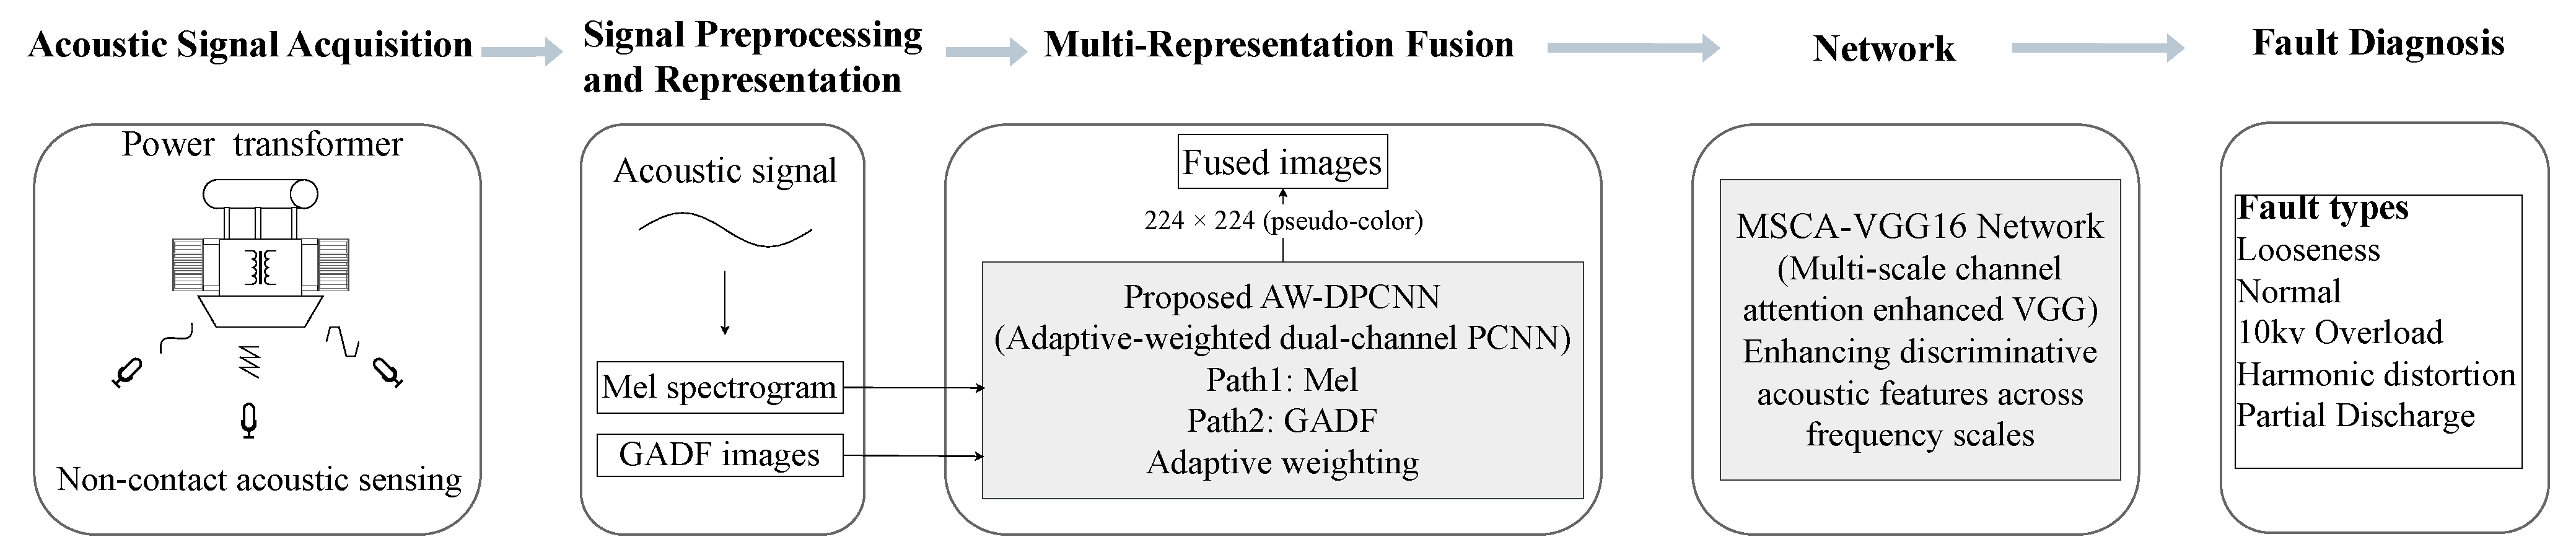
\includegraphics[width=\linewidth]{framework/framework}
\caption{Overall framework of the proposed transformer acoustic diagnosis method. The acoustic signal is first converted into Mel spectrogram and GADF images. These heterogeneous representations are then adaptively fused through the proposed AW-DPCNN mechanism. Finally, the fused feature is fed into the MSCA-VGG16 network for fault diagnosis.}
\label{framework}
\end{figure*}

\section{Acoustic Signal Representation}
\label{section2}
\subsection{Mel Spectrogram}
Acoustic signals generated by transformer faults are inherently nonstationary and exhibit frequency-dependent characteristics resulting from mechanical vibrations, electromagnetic forces, and partial discharge phenomena \cite{2025110731}, \cite{215108965}. Direct time-domain analysis is therefore insufficient to capture discriminative fault-related information. To address this issue, the Mel spectrogram is adopted as a perceptually motivated time--frequency representation that aligns with human auditory characteristics \cite{10091539}. The mapping from linear frequency $f$ to Mel frequency $f_{\mathrm{mel}}$ is defined as
\begin{equation}
f_{\mathrm{mel}} = 2595 \log_{10}\left(1 + \frac{f}{700}\right),
\end{equation}
where \( f \) denotes the original frequency, and \(f_{mel}\) represents the corresponding frequency on the Mel scale. 

Based on this mapping, the acoustic signal is first segmented into overlapping frames and transformed into the frequency domain using the STFT. The resulting power spectra are then projected onto a Mel-scale filter bank to obtain a perceptually meaningful spectral representation. To reduce the dynamic range of acoustic power spectra and improve feature robustness, logarithmic amplitude compression is applied. Consequently, the Mel spectrogram forms a compact two-dimensional representation that captures both the spectral distribution and temporal evolution of transformer acoustic emissions. Fig.~\ref{representation}(a) illustrates an example of a raw transformer acoustic signal and its corresponding Mel spectrogram, where fault-induced spectral energy redistribution can be clearly observed.

Although the Mel spectrogram effectively captures time–frequency characteristics of acoustic signals, it mainly reflects spectral energy distributions and may not fully describe the global temporal correlations of the signal. Therefore, an additional angular-domain representation is introduced in the following subsection.

\begin{figure}[!htbp]
	\centering
	\graphicspath{{representation/}}
	\begin{subfigure}{0.48\linewidth}
		\centering
		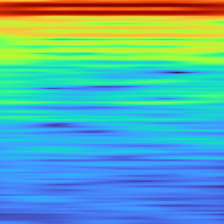
\includegraphics[width=\linewidth]{Normal_00000_mel}
		\caption{Mel spectrogram}
	\end{subfigure}
	\hfill
	\begin{subfigure}{0.48\linewidth}
		\centering
		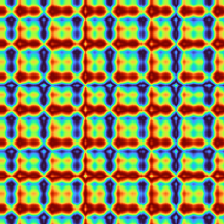
\includegraphics[width=\linewidth]{Normal_00000_gadf}
		\caption{GADF}
	\end{subfigure}
	
	\caption{Transformer acoustic signal representations.}
	\label{representation}
	
\end{figure}

\subsection{Gramian Angular Field}
The Gramian Angular Field (GAF) is a method that transforms time-series signals into images while preserving and encoding rich feature information \cite{11048665}. It was originally proposed to facilitate time-series classification through computer vision techniques \cite{10114345}, \cite{10281942}, and is described as follows.
\begin{enumerate}
\item The series $\boldsymbol{X}$ is first normalized to the interval \([-1,1]\). This operation produces a normalized one-dimensional sequence $\boldsymbol{\tilde X} = \{\tilde{x_1}, \tilde{x_2}, \ldots, \tilde{x_n}\} \quad (i = 1, 2, 3,\ldots)$, where each $\tilde{x}_i$ is computed as
\begin{equation}
	\tilde{x}_i = \frac{(x_i - \min \boldsymbol{X}) + (x_i - \max \boldsymbol{X})}{\max \boldsymbol{X} - \min \boldsymbol{X}}.
	\label{normalization}
\end{equation}
\item The normalized values $\tilde{x}_i$ are then encoded as angular coordinates in a polar system. Specifically, each $\tilde{x}_i$ is mapped to a polar angle $\phi_i$, while the corresponding radial coordinate $r_i$ represents the temporal order of the sequence. The transformation is defined as
\begin{equation}
	\begin{cases} 
		\phi_i = \arccos(\tilde{x}_i), & -1 \leq \tilde{x}_i \leq 1,  \tilde{x}_i \in \boldsymbol{\tilde X} \\
		r_i = \dfrac{i}{n}, & i = 1, \ldots, n 
	\end{cases},
	\label{cosine angle}
\end{equation}
where $\phi_i$ denotes the polar angle of the $i$-th point and $r_i$ represents its radial coordinate.
\item Finally, the GAF is constructed by aggregating the phase angles obtained from the polar coordinate transformation using either the sum or the difference of these angles. This results in two variants, i.e., the GASF, denoted as $\boldsymbol{G_s}$, and the GADF, denoted as $\boldsymbol{G_d}$. Their formulations are defined as
\begin{equation}
	\boldsymbol{G_s}(i,j) = \cos(\phi_i + \phi_j), \quad i,j = 1,\ldots,n
	\label{eq:gasf}
\end{equation}
\begin{equation}
	\boldsymbol{G_d}(i,j) = \sin(\phi_i - \phi_j), \quad i,j = 1,\ldots,n.
	\label{eq:gadf}
\end{equation}
\end{enumerate}

In this study, the GADF representation is introduced to complement the Mel spectrogram by encoding temporal correlation structures of the acoustic signal. Compared with GASF, GADF focuses on angular differences rather than amplitude summation, which improves sensitivity to abrupt temporal variations and asymmetric dynamic patterns \cite{11278186}. This property is beneficial for transformer acoustic fault diagnosis, where abnormal operating conditions often produce irregular temporal fluctuations in the acoustic signals.

As shown in Fig.~\ref{representation}(b), the GADF encodes structured temporal dependencies from acoustic signals under normal operating conditions. The resulting image exhibits regular and symmetric patterns, reflecting stable temporal correlations and consistent signal dynamics. These structured textures indicate that the underlying acoustic signals possess strong periodicity and steady-state behavior, which are effectively captured by the angular transformation. Such characteristics provide discriminative cues for distinguishing normal conditions from fault-induced irregular patterns.

\section{Adaptive Weighted Dual-Channel PCNN for Multi-Representation Fusion}
\label{section3}
As discussed above, the Mel spectrogram and GADF provide fundamentally different yet complementary representations of transformer acoustic signals. Specifically, the Mel spectrogram primarily characterizes local time--frequency energy distributions and perceptually relevant spectral patterns, whereas the GADF emphasizes global temporal dependencies and dynamic correlation structures. Owing to their distinct statistical properties and structural characteristics, directly combining these heterogeneous representations using conventional convolution or simple feature concatenation may fail to effectively capture their cross-modal relationships and complementary fault information.

To address this issue, the proposed AW-DPCNN introduces a PCNN-inspired fusion mechanism to enhance heterogeneous representation integration. The pulse coupling characteristic of PCNN enables dynamic interaction among neighboring feature responses, allowing salient structures shared across Mel and GADF representations to be synchronously enhanced while suppressing irrelevant or inconsistent activations~\cite{Li_2018}. Such a mechanism is particularly suitable for acoustic representation fusion, where local spectral textures and global temporal correlation patterns coexist across different feature domains~\cite{Kang_2021}. Moreover, the adaptive weighting strategy further regulates the contribution of each representation according to their fault-sensitive responses, thereby improving feature complementarity and discriminative capability.

Building upon these characteristics, the proposed AW-DPCNN integrates dual-channel processing, adaptive weighting, and multi-scale convolution to effectively model cross-representation dependencies and hierarchical feature interactions between Mel and GADF representations, ultimately enhancing transformer fault diagnosis performance.

\subsection{Input normalization}
To eliminate scale differences between two representations, each input is first normalized to the interval $[0,1]$ as
\begin{equation}
	\boldsymbol{\tilde{S}}_k(i,j) = \frac{\boldsymbol{S}_k(i,j) - \min\limits_{i,j} (\boldsymbol{S}_k(i,j))}{\max\limits_{i,j} (\boldsymbol{S}_k(i,j)) - \min\limits_{i,j} (\boldsymbol{S}_k(i,j)) + \epsilon}, k\in\{1,2\}
	\label{eq:normalization}
\end{equation}
where $\boldsymbol{S}_k(i,j)$ denotes the value of the $k$-th input representation at spatial location $(i,j)$, corresponding to the Mel spectrogram ($k=1$) or the GADF image ($k=2$). The variables $i$ and $j$ denote the pixel indices, and $\epsilon$ is a small positive constant preventing division by zero.

\subsection{Contrast-Guided Adaptive Weighting}
For each representation, the local mean of the normalized representation is computed as
\begin{equation}
	\boldsymbol{\mu}_k(i,j) = \frac{1}{|\boldsymbol{\Omega}|}
	\sum_{(p,q)\in \boldsymbol{\Omega}} \boldsymbol{\tilde{S}}_k(p,q),
	\label{eq:local_mean}
\end{equation}
where $\boldsymbol{\Omega}$ denotes the local neighborhood centered at each pixel location, and $|\boldsymbol{\Omega}|$ represents the number of elements in the neighborhood.

The corresponding local contrast is defined as
\begin{equation}
	C_k(i,j) = \sqrt{ \left| \mathbb{E}_\Omega \left[ \tilde{S}_k^2 \right] - \mu_k^2(i,j) \right| },
	\label{eq:eq:local_contrast}
\end{equation}
where $\mathbb{E}[\cdot]$ denotes local averaging within $\boldsymbol{\Omega}$.

Local contrast operators $C_1(i,j)$ and $C_2(i,j)$ are computed to quantify the saliency of Mel and GADF representations at each spatial location. To emphasize the dominant representation, a contrast amplification factor $\gamma$ is introduced to construct adaptive fusion weights as follows
\begin{equation}
	\beta_1(i,j) = 
	\frac{\gamma C_1(i,j)}
	{\gamma C_1(i,j) + C_2(i,j) + \epsilon},
	\label{eq:beta1}
\end{equation}
\begin{equation}
	\beta_2(i,j) = 
	\frac{C_2(i,j)}
	{\gamma C_1(i,j) + C_2(i,j) + \epsilon},
	\label{eq:beta2}
\end{equation}
the above formulation ensures $\beta_1(i,j) + \beta_2(i,j) \approx 1$, enabling contrast-driven dynamic weighting.

\subsection{Dual-Channel PCNN}
Let $\boldsymbol{L}^n(i,j)$, $\boldsymbol{T}^n(i,j)$, and $\boldsymbol{Y}^n(i,j)$ denote the linking term, dynamic threshold, and binary pulse output, respectively, where $n$ denotes the current iteration and $n \in [1, N]$, with $N$ being the total number of iterations. The neural states are initialized as
\begin{equation}
	\boldsymbol{L}^0(i,j) = \boldsymbol {0}, \quad 
	\boldsymbol{T}^0(i,j) = \boldsymbol {0}, \quad 
	\boldsymbol{Y}^0(i,j) = \boldsymbol {0}.
	\label{eq:initialization}
\end{equation}

At the $n$-th iteration, the external stimulus from two channels is defined as
\begin{equation}
	\boldsymbol{F}_1^n(i,j) = (\boldsymbol{W}_1 * \boldsymbol{Y}^{n-1})(i,j) + \boldsymbol{\tilde{S}}_1(i,j)
	\label{eq:f1_update}
\end{equation}
\begin{equation}
	\boldsymbol{F}_2^n(i,j) = (\boldsymbol{W}_2 * \boldsymbol{Y}^{n-1})(i,j) + \boldsymbol{\tilde{S}}_2(i,j),
	\label{eq:f2_update}
\end{equation}
where $\boldsymbol{W}_1$ and $\boldsymbol{W}_2$ denote the convolutional kernels corresponding to the Mel and GADF channels, respectively, and $*$ represents the convolution operation. Considering the distinct structural characteristics of the two representations, representation-specific convolutional kernels are introduced in the dual-channel architecture. Specifically, stripe-shaped kernels are applied to the Mel channel to emphasize frequency continuity and harmonic structures, while symmetric kernels are used for the GADF channel to capture temporal periodicity and global correlation patterns.

The internal linking state is updated by
\begin{equation}
	\boldsymbol{L}^n(i,j) = e^{-\alpha_L} \boldsymbol{L}^{n-1}(i,j) + (\boldsymbol{M} * \boldsymbol{Y}^{n-1})(i,j),
	\label{eq:linking_update}
\end{equation}
where $\alpha_L$ is the decay coefficient and $\boldsymbol M$ represents the coupling matrix.

The total neuron input is then given by
\begin{equation}
	\boldsymbol{U}^n(i,j) = \boldsymbol{L}^n(i,j)\Big(1 + \beta_1 \boldsymbol{F}_1^n(i,j)\Big)
	\Big(1 + \beta_2 \boldsymbol{F}_2^n(i,j)\Big) + \sigma,
	\label{eq:internal_activity}
\end{equation}
where $\sigma$ is a stabilization constant.

The pulse output is determined by a threshold comparison as follows
\begin{equation}
	\boldsymbol{Y}^n(i,j) =
	\begin{cases}
		1, & \boldsymbol{U}^n(i,j) > \boldsymbol{T}^{n-1}(i,j) \\
		0, & \text{otherwise}
	\end{cases}.
	\label{eq:pulse_output}
\end{equation}

The dynamic threshold evolves according to
\begin{equation}
	\boldsymbol{T}^n(i,j) = e^{-\alpha_T} \boldsymbol{T}^{n-1}(i,j) + V_T \boldsymbol{Y}^n(i,j),
	\label{eq:threshold_update}
\end{equation}
where $\alpha_T$ controls threshold decay and $V_T$ is the amplification coefficient.

\subsection{Fused Representation}
The accumulated neural response after $N$ iterations is
\begin{equation}
	\boldsymbol{U}_{\mathrm{sum}}(i,j)=\sum_{n=1}^{N} \boldsymbol{U}^{n}(i,j),
\end{equation}
and the final fused representation is obtained via normalization as
\begin{equation}
	\boldsymbol{F}(i,j)=
	\frac{\boldsymbol{U}_{\mathrm{sum}}(i,j)-\min\limits_{i,j} \boldsymbol{U}_{\mathrm{sum}}(i,j)}
	{\max\limits_{i,j} \boldsymbol{U}_{\mathrm{sum}}(i,j)-\min\limits_{i,j} \boldsymbol{U}_{\mathrm{sum}}(i,j)+\epsilon}.
\end{equation}

Through the proposed adaptive fusion mechanism, Mel and GADF representations are no longer combined with fixed weights. Instead, the neuron state is dynamically modulated in a demand-driven manner, i.e., regions dominated by spectral variations are mainly governed by Mel, while regions with stronger temporal correlations rely more on GADF. This adaptive strategy effectively suppresses fusion artifacts while enhancing the discriminative capability of acoustic representations.

The overall architecture of the proposed AW-DPCNN is illustrated in Fig.~\ref{AW-DPCNN}. By integrating Mel spectral perception and GADF temporal encoding within a unified adaptive fusion framework, the proposed AW-DPCNN produces robust and discriminative acoustic representations for transformer fault diagnosis. The qualitative effectiveness of the proposed adaptive fusion mechanism is further analyzed through feature visualization in Section~\ref{section5}.
\begin{figure}
	\centering
	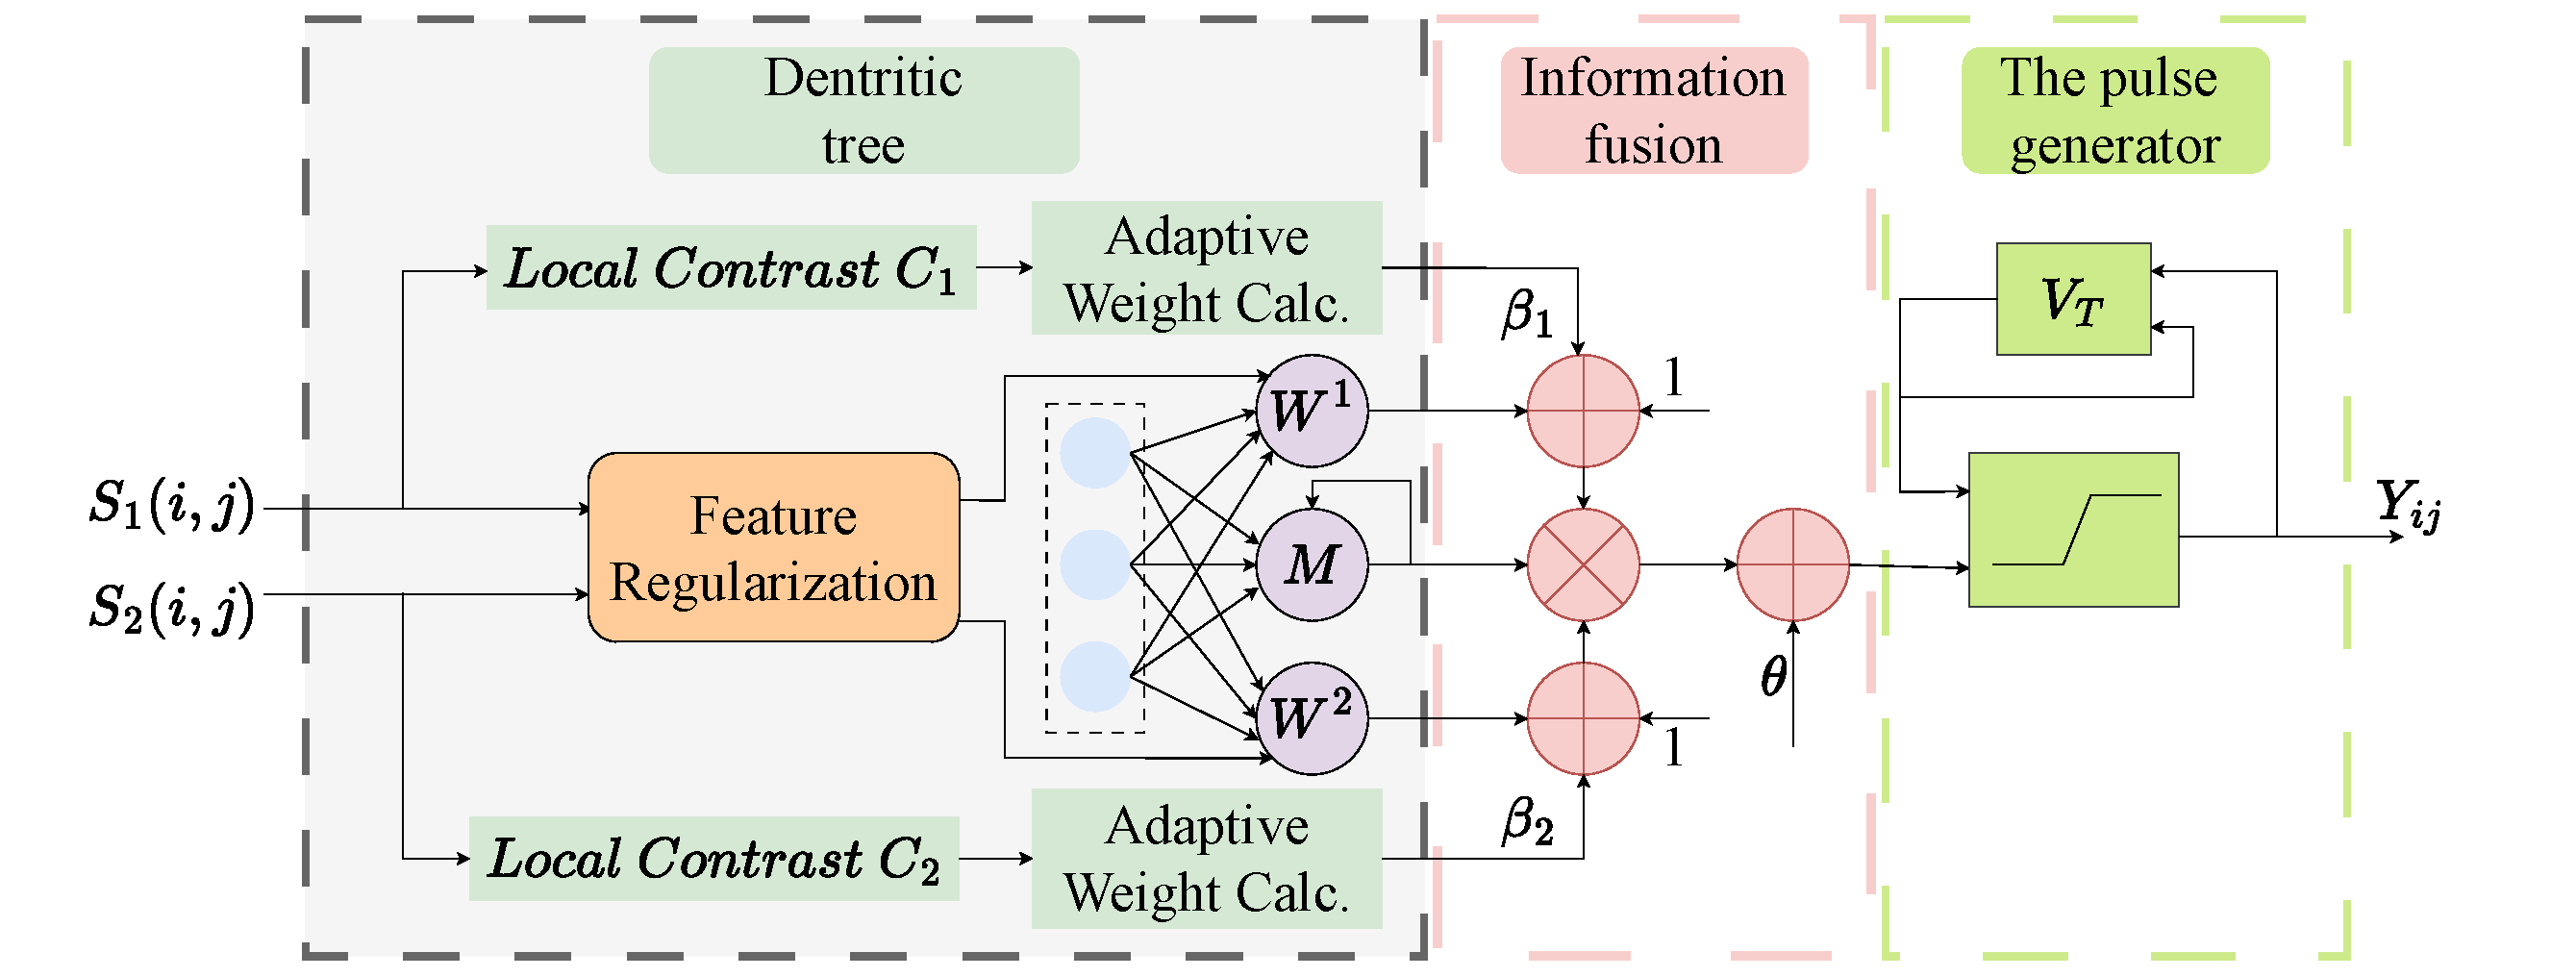
\includegraphics[width=\linewidth]{AW-DPCNN/AW-DPCNN}
	\caption{Architecture of the proposed adaptive weighted dual-channel PCNN (AW-DPCNN) for multi-representation acoustic signal fusion.}
	\label{AW-DPCNN}                       
\end{figure}

\section{MSCA-VGG16 for Fused representations Classification}
\label{section4}
The fused representations simultaneously encode local spectral energy variations captured by Mel spectrograms and global temporal dependency structures derived from GADF encoding. Such representations exhibit heterogeneous characteristics with distinct statistical distributions and spatial patterns, where Mel spectrograms emphasize localized time–frequency energy variations, while GADF images reveal long-range temporal correlation structures. However, conventional convolutional neural networks typically rely on fixed receptive fields and single-scale feature extraction, which limits their ability to simultaneously capture fine-grained local details and global structural dependencies within the fused feature space. As a result, these models may not fully exploit the complementary information contained in the heterogeneous representations. To address this limitation, a structurally aware discriminative network, termed MSCA-VGG16, is developed to better align the network perception with the intrinsic properties of the fused representations, thereby enhancing representation capability and improving fault classification performance.

Let the fused representation be denoted as 
\begin{equation}
	\boldsymbol{X} \in \mathbb{R}^{H \times W \times C},
\end{equation}
where $H$, $W$, and $C$ represent the spatial height, width, and number of channels of the extracted feature map, respectively, the proposed MSCA-VGG16 network transforms $\boldsymbol{X}$ into a compact discriminative embedding and the corresponding class logits. The overall mapping can be formulated as
\begin{equation}
	\hat{\mathbf{y}} = \mathcal{F}_{cls}\big(\mathcal{E}\big(\mathcal{P}\big(\mathcal{M}\big(\mathcal{B}(\boldsymbol{X})\big)\big)\big)\big),
	\label{eq:cls_pipeline}
\end{equation}
where $\mathcal{B}(\cdot)$ denotes the VGG16 backbone, $\mathcal{M}(\cdot)$ denotes the multi-scale channel attention module, $\mathcal{P}(\cdot)$ represents global pooling and flattening, $\mathcal{E}(\cdot)$ denotes the embedding projection, and $\mathcal{F}_{cls}(\cdot)$ denotes the final classifier.

This design prioritizes structural alignment with fused acoustic representations instead of merely increasing network depth. The main components are described below.

\subsection{Multi-Scale Channel Attention Module}
Given input $\boldsymbol{X}$, hierarchical convolutional features are obtained as
\begin{equation}
	\boldsymbol{F} = \mathcal{B}(\boldsymbol{X}), \quad \boldsymbol{F} \in \mathbb{R}^{H \times W \times C}.
	\label{eq:feature_map}
\end{equation}

The backbone performs progressive spatial abstraction through stacked convolutions and max-pooling operations, generating high-level representations while preserving structural continuity in the fused time–frequency image.

The fused representations contain fault-dependent patterns that span different temporal and spectral scales. Some fault signatures are manifested as localized high-energy regions, while others present as long-range correlations across time or frequency. To align the network perception with these characteristics, a structure-aligned enhancement module is incorporated after the convolutional backbone. Instead of relying on a single receptive field, multiple convolutional kernels with different effective receptive fields are employed to capture complementary fault patterns, i.e.,
\begin{equation}
	\boldsymbol{F}_{ms} = \sum_{i=1}^{S} \psi_i(\boldsymbol{F}),
	\label{eq:multi_scale_feature}
\end{equation}
where $S$ denotes the number of multi-scale branches, $\psi_i(\cdot)$ denotes convolutional operators with different receptive fields. In this study, three convolutional branches are adopted, including $3\times3$, $5\times5$, and dilated $3\times3$ convolutions, to capture local, mid-range, and long-range fault patterns. Each operator preserves the channel dimensionality of the input feature map. The outputs of these branches are fused via element-wise summation, enabling the network to capture complementary fault signatures across multiple spatial ranges.

The aggregated feature map is then normalized and activated as
\begin{equation}
	\boldsymbol{F}_{act} = \delta\big(\text{BN}(\boldsymbol{F}_{ms})\big),
	\label{eq:active_feature}
\end{equation}
where $\delta(\cdot)$ denotes the ReLU function.

Furthermore, channel-wise recalibration is applied to emphasize informative frequency-related responses while suppressing redundant or noise-dominated channels. The proposed mechanism allows the network to selectively focus on discriminative fault components, which is particularly beneficial for acoustic fault diagnosis where frequency band importance varies across fault types. 

The resulting channel descriptor vector is denoted as
\begin{equation}
	\boldsymbol{z} = [z_1, z_2, \dots, z_C]^T, \quad c \in \{1,2,\dots,C\}
\end{equation}
and global channel descriptors are computed as
\begin{equation}
	z_c = \frac{1}{HW} \sum_{i=1}^{H} \sum_{j=1}^{W} \boldsymbol{F}_{act}(i, j, c),
	\label{eq:channel_embedding}
\end{equation}
and channel weights are obtained via
\begin{equation}
	\boldsymbol{s} = \sigma\big(\boldsymbol{W}_2 \delta(\boldsymbol{W}_1 \boldsymbol{z})\big),
	\label{eq:attention_score}
\end{equation}
where $\boldsymbol{W}_1 \in \mathbb{R}^{\frac{C}{r}\times C}$, $\boldsymbol{W}_2 \in \mathbb{R}^{C\times \frac{C}{r}}$, $r$ is the reduction ratio, and $\sigma(\cdot)$ denotes the sigmoid function. 

The refined feature map becomes
\begin{equation}
	\boldsymbol{F}_{att}(i,j,c) = \boldsymbol{s}_c \cdot \boldsymbol{F}_{act}(i,j,c).
	\label{eq:attention_feature}
\end{equation}
where $\boldsymbol{s} = [s_1, s_2, \dots, s_C]^T$ represents the
channel attention weights.

The proposed mechanism aligns receptive fields with heterogeneous fault patterns and dynamically emphasizes discriminative spectral–temporal components introduced by the fused time–frequency representation.

\subsection{Compact and Discriminative Embedding for Classification}
In conventional VGG16 architectures, large fully connected layers are employed to map convolutional features directly to class labels \cite{9770845}. While effective for large-scale image datasets, such designs often lead to excessive redundancy and limited interpretability when applied to fault diagnosis tasks. To address this issue, a compact discriminative embedding head is introduced to replace the original over-parameterized classification layers. Specifically, high-dimensional convolutional features are first projected into a lower-dimensional embedding space through a feature reconstruction layer, followed by normalization and nonlinear activation. This embedding head serves as a feature refinement stage rather than a simple classifier.

The refined feature map is further transformed into a compact feature vector through global average pooling followed by flattening
\begin{equation}
	\boldsymbol{f}_0 = \text{Flatten}\big(\text{AvgPool}(\boldsymbol{F}_{att})\big).
	\label{eq:flatten_feature}
\end{equation}

A fully connected projection generates high-level features as follows
\begin{equation}
	\boldsymbol{f}_1 = \delta\big(\boldsymbol{W}_{fc1} \boldsymbol{f}_0\big),
	\label{eq:fc1_feature}
\end{equation}
where $\boldsymbol{W}_{fc1}$ represents the weight matrix of the first fully
connected projection layer and $\delta(\cdot)$ denotes the ReLU
activation function.

Instead of directly applying a large classifier, a compact embedding layer reshapes the feature space, i.e.,
\begin{equation}
	\boldsymbol{e} = \delta\big(\text{BN}(\boldsymbol{W}_e \boldsymbol{f}_1)\big), \quad \boldsymbol{e} \in \mathbb{R}^d
	\label{eq:embedding}
\end{equation}
where $\boldsymbol{W}_e$ denotes the embedding projection matrix and
$d$ represents the dimensionality of the compact embedding space.

Let $\boldsymbol{y}$ and $\hat{\boldsymbol{y}}$ denote the ground-truth label
vector and the predicted probability vector, respectively. The final
prediction is obtained as
\begin{equation}
	\hat{\boldsymbol{y}} = \text{softmax}(\boldsymbol{W}_c \boldsymbol{e}),
\end{equation}
where $\boldsymbol{W}_c \in \mathbb{R}^{K \times d}$ is the classification weight matrix, $K$ denotes the number of fault categories.

The network is optimized using cross-entropy loss as follows
\begin{equation}
	\mathcal{L} = -\sum_{k=1}^{K} \boldsymbol{y}_k \log \hat{\boldsymbol{y}}_k.
	\label{eq:cross_entropy_loss}
\end{equation}

By projecting high-dimensional convolutional features into a compact latent space, the embedding layer enhances intra-class compactness and inter-class separability while reducing parameter redundancy. The proposed MSCA-VGG16 framwork is presented in Fig.~\ref{MSCA-VGG}.
\begin{figure}
	\centering
	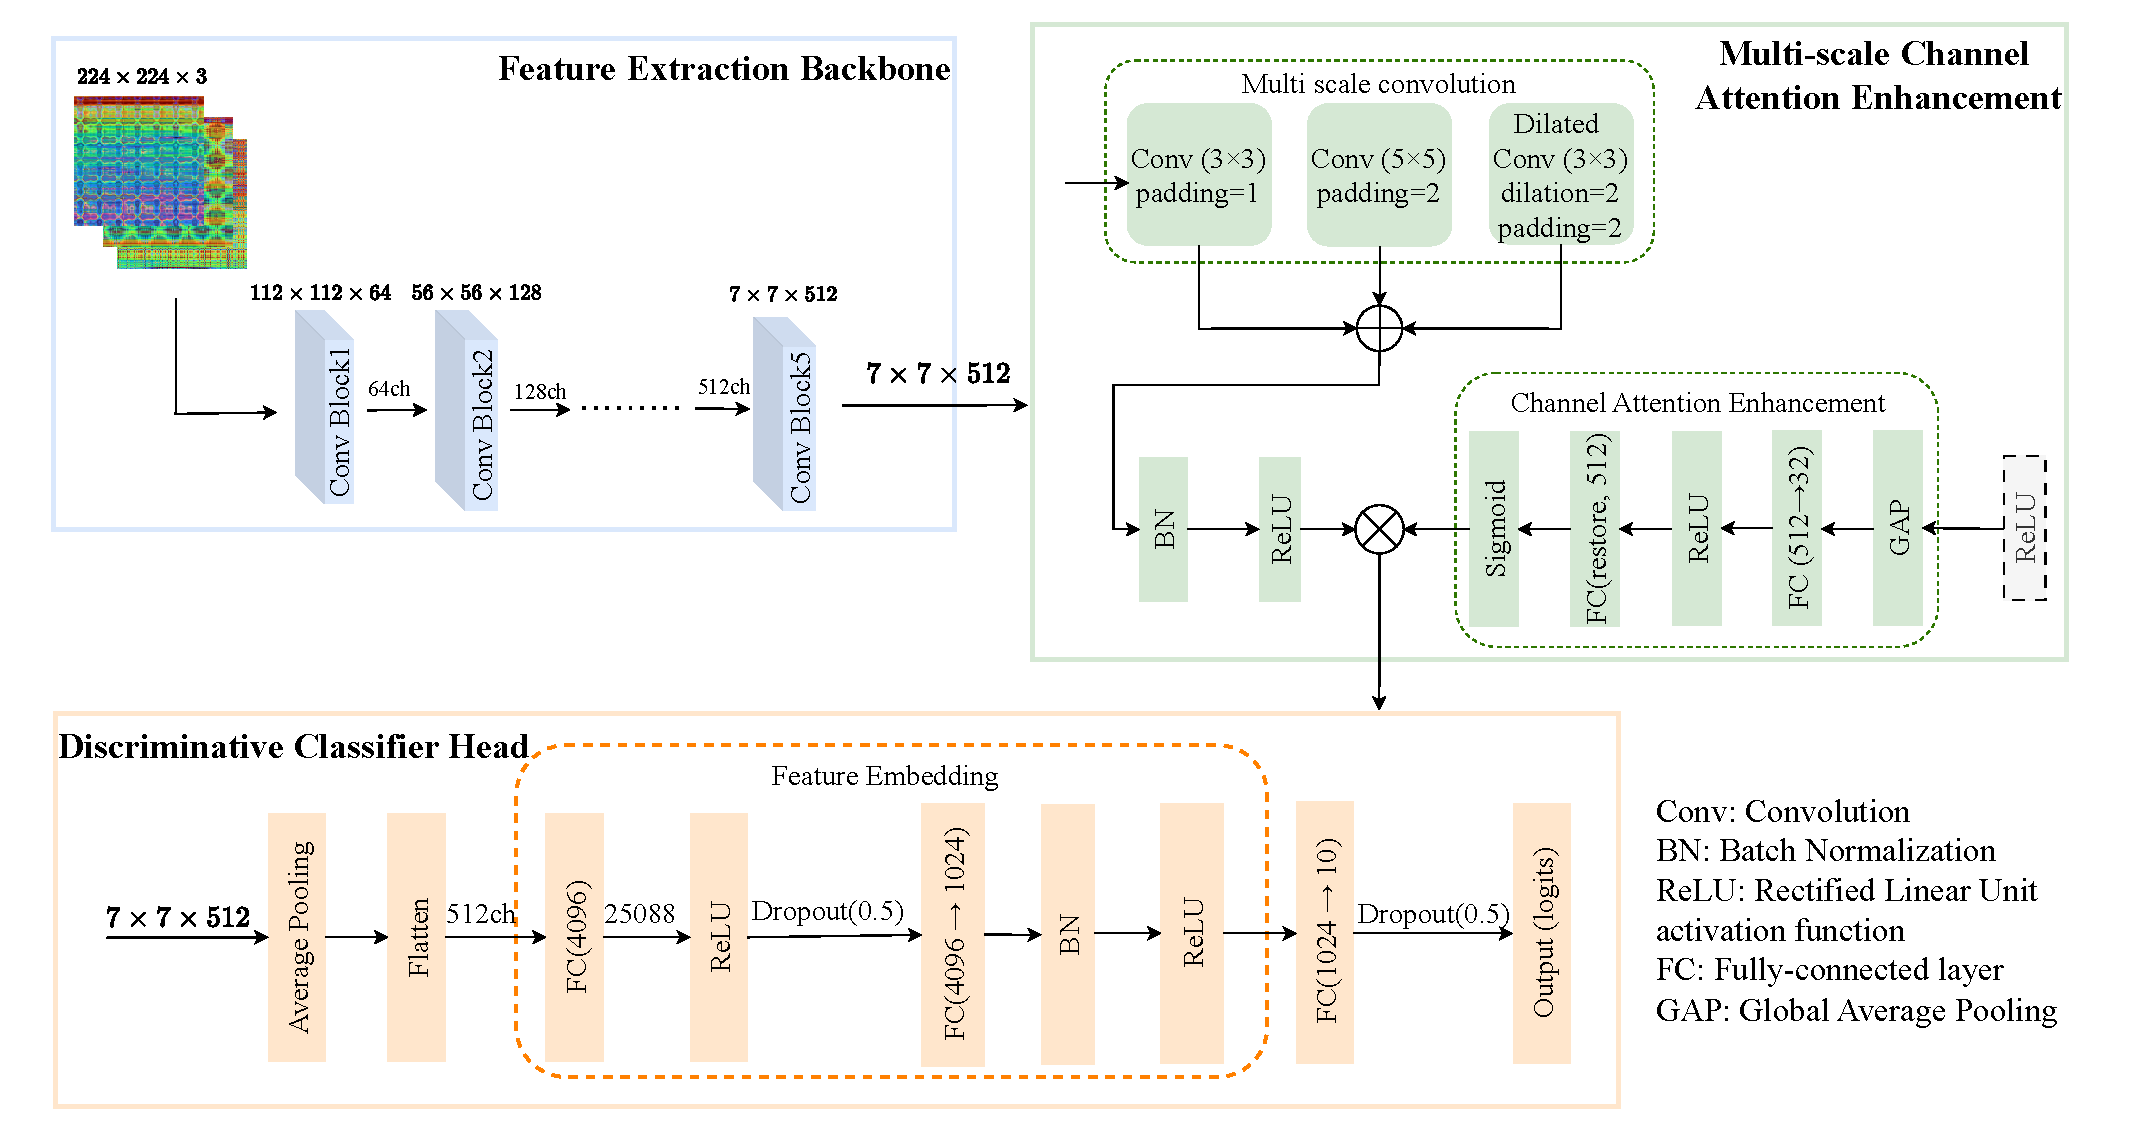
\includegraphics[width=\textwidth]{MSCA-VGG16/MSCA-VGG16}
	\caption{Overall architecture of the proposed MSCA-VGG16 network for transformer fault classification.}
	\label{MSCA-VGG}
\end{figure}

\section{Experimental Setup and Performance Evaluation}
\label{section5}
\subsection{Dataset Construction and Preprocessing}
An experimental platform was established to collect acoustic signals from power transformers operating in a real substation environment. Among several transformers deployed at different locations, a series of 220 kV transformers were selected for acoustic data acquisition due to their prominent vibration-induced acoustic emissions. As illustrated in Fig.~\ref{fig:equipment}, the acoustic acquisition system consists of an omnidirectional microphone mounted on a tripod and connected to a data acquisition device via a USB interface for both power supply and signal transmission. To ensure stable signal capture while reducing environmental interference, the microphone was positioned approximately 1.2~m in front of the transformer tank.
\begin{figure}
	\centering
	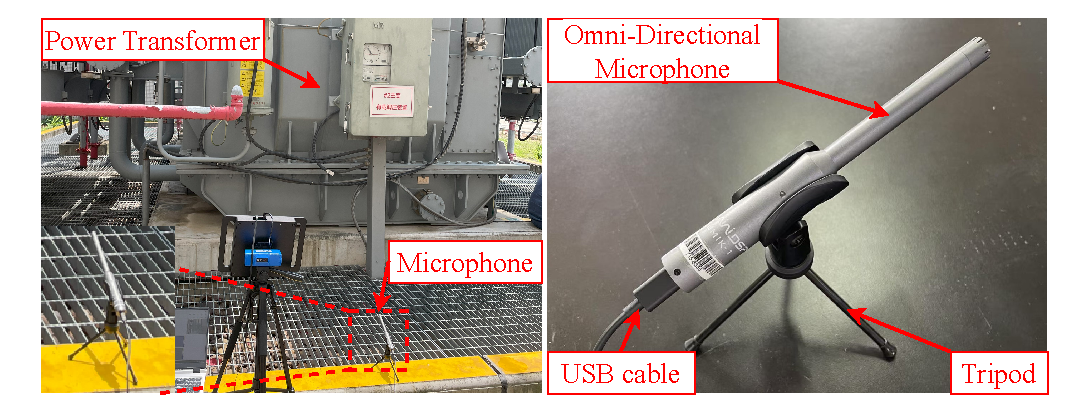
\includegraphics[width=\linewidth]{equipment/equipment}
	\caption{Experimental platform of acoustic signal acquisition.}
	\label{fig:equipment}
\end{figure}

All acoustic data were recorded across multiple independent acquisition sessions under different operating conditions. The continuous audio signals were first resampled to a uniform sampling rate of 44.1kHz to ensure consistency. Each recording was then segmented into fixed-length clips of 1s with 60\% overlap. To prevent data leakage caused by temporal correlation between overlapping segments, dataset partitioning was conducted at the recording-session level rather than at the segment level. Specifically, all segments derived from the same recording session were assigned exclusively to either the training, validation, or test subset. The dataset is divided into training, validation, and test subsets with a ratio of 60\%, 20\%, and 20\%, respectively, using a fixed random seed to ensure reproducibility and strict independence between the subsets.

The collected acoustic signals were categorized into multiple classes corresponding to different transformer operating conditions, including normal operation and several typical fault states, as shown in Table~\ref{tab:operating_conditions}. Each acoustic segment was independently labeled according to the operating condition during the recording period. The detailed composition of the dataset, including the number of samples in each subset, is summarized in Table~\ref{dataset}.


\begin{table}
	\caption{Transformer Operating Conditions and Corresponding Labels}
	\centering
	\begin{tabular}{ll}
		\toprule
		Label & Operating Condition \\
		\midrule
		N0 & 10 kV Overload \\
		N1 & 30\% Fifth Harmonic Distortion \\
		N2 & 30\% Seventh Harmonic Distortion \\
		N3 & 30\% Third Harmonic Distortion \\
		N4 & Loosen \\
		N5 & Normal \\
		N6 & Partial Discharge \\
		N7 & Pure Fifth Harmonic Distortion \\
		N8 & Pure Seventh Harmonic Distortion \\
		N9 & Pure Third Harmonic Distortion \\
		\bottomrule
	\end{tabular}
	\label{tab:operating_conditions}
\end{table}

\begin{table}
	\centering
	\caption{Composition of the Transformer Acoustic Dataset}
	\label{dataset}
	\begin{tabular}{l c c c c c c c c c c c}
		\toprule
		\multirow{2}{*}{Datasets} & 
		\multirow{2}{*}{Total} & 
		\multicolumn{10}{c}{Number of Samples per Class (N0–N9)} \\
		\cmidrule(lr){3-12}
		&  & N0 & N1 & N2 & N3 & N4 & N5 & N6 & N7 & N8 & N9 \\
		\midrule
		Training set & 8924 & 881 & 880 & 881 & 880 & 1002 & 880 & 880 & 880 & 880 & 880\\
		Validating set & 3410 & 440 & 294 & 441 & 294 & 441 & 324 & 294 & 294 & 294 & 294\\
		Testing set & 4115 & 441 & 294 & 441 & 294 & 441 & 881 & 294 & 441 & 294 & 294 \\
		\bottomrule
	\end{tabular}
\end{table}

Fig.~\ref{Fig: Fused images} illustrates the representations of different transformer operating conditions before and after adaptive fusion. The Mel spectrogram primarily reflects frequency-domain energy distributions, where harmonic-related faults exhibit distinct banded patterns. In contrast, GADF images encode temporal correlations and periodic structures of the acoustic signals, revealing complementary information that is not explicitly captured in the Mel domain.
\begin{figure}
	\centering
	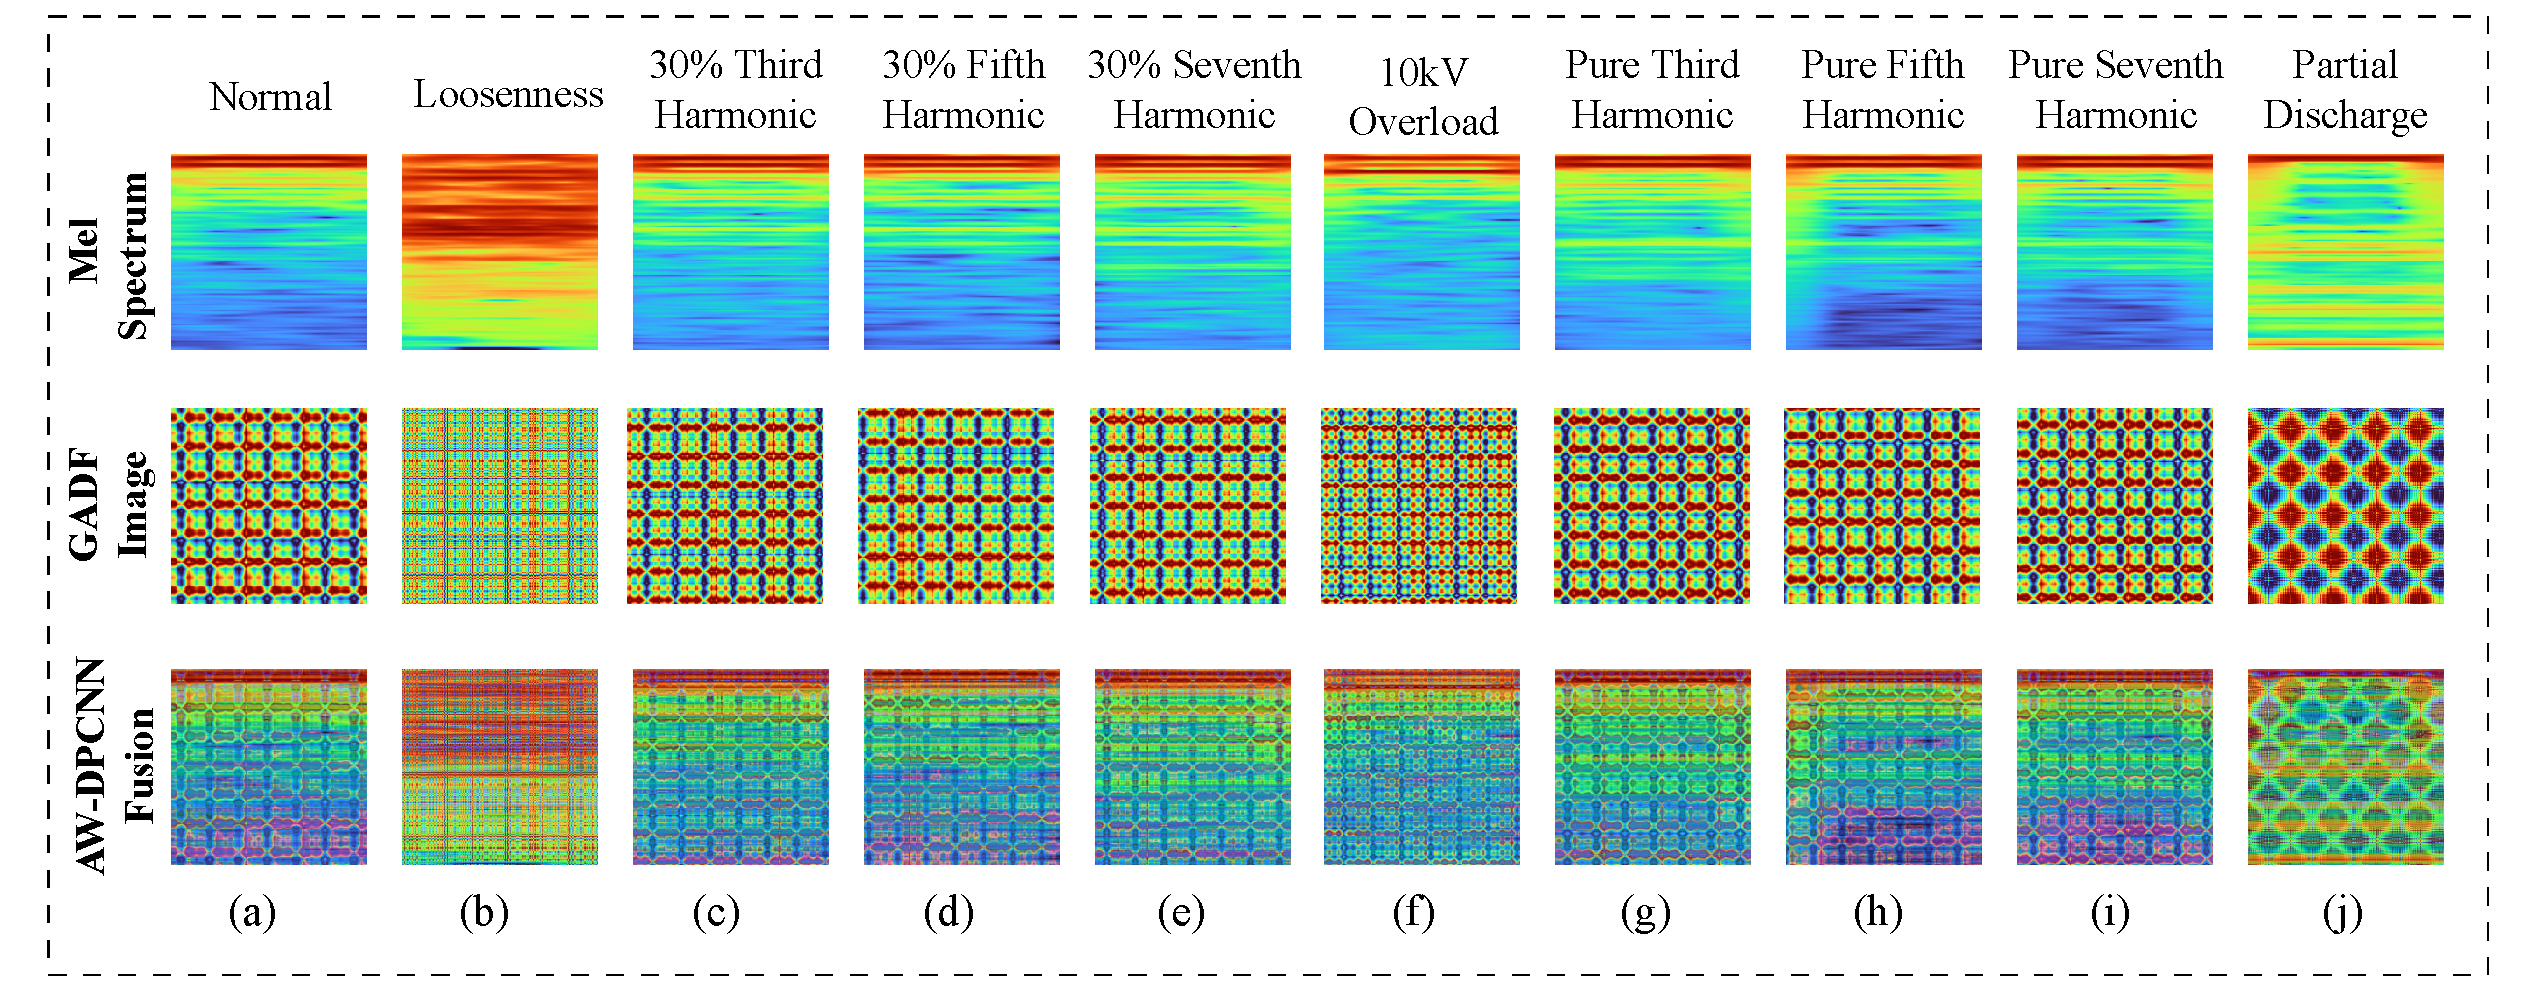
\includegraphics[width=\textwidth]{Fused images/Fused images}
	\caption{Visualization of Mel spectrograms, GADF images, and adaptively fused representations generated by the proposed AW-DPCNN under different transformer operating conditions. (a) Normal, (b) Loosen, (c) 30\% Third Harmonic Distortion, (d) 30\% Fifth Harmonic Distortion,  (e) 30\% Seventh Harmonic Distortion, (f) 10kV Overload, (g) Pure Third Harmonic, (h) Pure Fifth Harmonic, (i) Pure Seventh Harmonic, and (j) Partial Discharge.}
	\label{Fig: Fused images}
\end{figure}     

After processing by the proposed AW-DPCNN, the fused feature maps exhibit enhanced structural clarity and improved discrimination among different fault types. Notably, background noise and redundant patterns are effectively suppressed, while salient fault-related features are preserved and highlighted. This qualitative analysis demonstrates that the AW-DPCNN is capable of adaptively integrating frequency-domain and temporal-domain information, thereby generating more informative representations for subsequent fault classification.

\subsection{Implementation Details and Evaluation Metrics}
The raw acoustic signals are converted into Mel spectrograms and GADF images, which are subsequently fused using the proposed AW-DPCNN to generate pseudo-color RGB images of size $224 \times 224$. These fused representations serve as the input to the MSCA-VGG16 network. All experiments follow a unified training protocol. During each ablation study, only one factor is modified while all other settings remain unchanged. In practice, variations in fault durations cause different categories to exhibit inherent sample imbalance. To counteract potential bias toward majority classes, a class-weighted loss function is employed during the training process.

The experiments in this study were conducted on a system equipped with an Intel i9-14900K CPU and an NVIDIA RTX 5090 GPU. The software environment was based on PyTorch 2.11 and CUDA 12.8. To comprehensively evaluate the classification performance, several commonly used metrics are adopted, including accuracy, precision, recall, F1-score, balanced accuracy (B-Acc), G-mean, and Cohen’s kappa. Let $C$ denote the number of classes and $m_{ij}$ represent the element of the confusion matrix indicating the number of samples belonging to class $i$ but predicted as class $j$.
\begin{enumerate}
	\item \textbf{Accuracy}
	The overall classification accuracy is defined as
	\begin{equation}
		\mathrm{Accuracy} =
		\frac{\sum_{c=1}^{C} m_{cc}}
		{\sum_{i=1}^{C}\sum_{j=1}^{C} m_{ij}}.
	\end{equation}
	\item \textbf{Precision, Recall, and F1-score}
	For class $c$, Precision and Recall are defined as
	\begin{equation}
		\mathrm{Precision}_c =
		\frac{m_{cc}}
		{\sum_{i=1}^{C} m_{ic}},
	\end{equation}
	\begin{equation}
		\mathrm{Recall}_c =
		\frac{m_{cc}}
		{\sum_{j=1}^{C} m_{cj}}.
	\end{equation}
	The corresponding F1-score is given by
	\begin{equation}
		\mathrm{F1}_c =
		\frac{2\,\mathrm{Precision}_c \cdot \mathrm{Recall}_c}
		{\mathrm{Precision}_c + \mathrm{Recall}_c}.
	\end{equation}
	The macro-averaged F1-score is calculated as
	\begin{equation}
		\mathrm{F1}_{macro} =
		\frac{1}{C}\sum_{c=1}^{C}\mathrm{F1}_c.
	\end{equation}
	\item \textbf{Balanced Accuracy (B-Acc)}
	Balanced accuracy is defined as the average recall across all classes
	\begin{equation}
		\mathrm{B\text{-}Acc} =
		\frac{1}{C}\sum_{c=1}^{C}\mathrm{Recall}_c.
	\end{equation}
	\item \textbf{G-mean}
	The geometric mean of class-wise recall is defined as
	\begin{equation}
		\mathrm{G\text{-}Mean} =
		\left(\prod_{c=1}^{C}\mathrm{Recall}_c\right)^{\frac{1}{C}}.
	\end{equation}
	\item \textbf{Cohen’s kappa}
	The observed agreement is
	\begin{equation}
		P_o =
		\frac{\sum_{c=1}^{C} m_{cc}}
		{\sum_{i=1}^{C}\sum_{j=1}^{C} m_{ij}},
	\end{equation}
	and the expected agreement is
	\begin{equation}
		P_e =
		\frac{\sum_{c=1}^{C}
			\left(\sum_{j=1}^{C} m_{cj}\right)
			\left(\sum_{i=1}^{C} m_{ic}\right)}
		{\left(\sum_{i=1}^{C}\sum_{j=1}^{C} m_{ij}\right)^2}.
	\end{equation}
	Thus, Cohen’s kappa coefficient is defined as
	\begin{equation}
		\kappa =
		\frac{P_o - P_e}{1 - P_e}.
	\end{equation}
\end{enumerate}

	\begin{figure*}
		\centering
		\begin{subfigure}{0.48\textwidth}
			\centering
			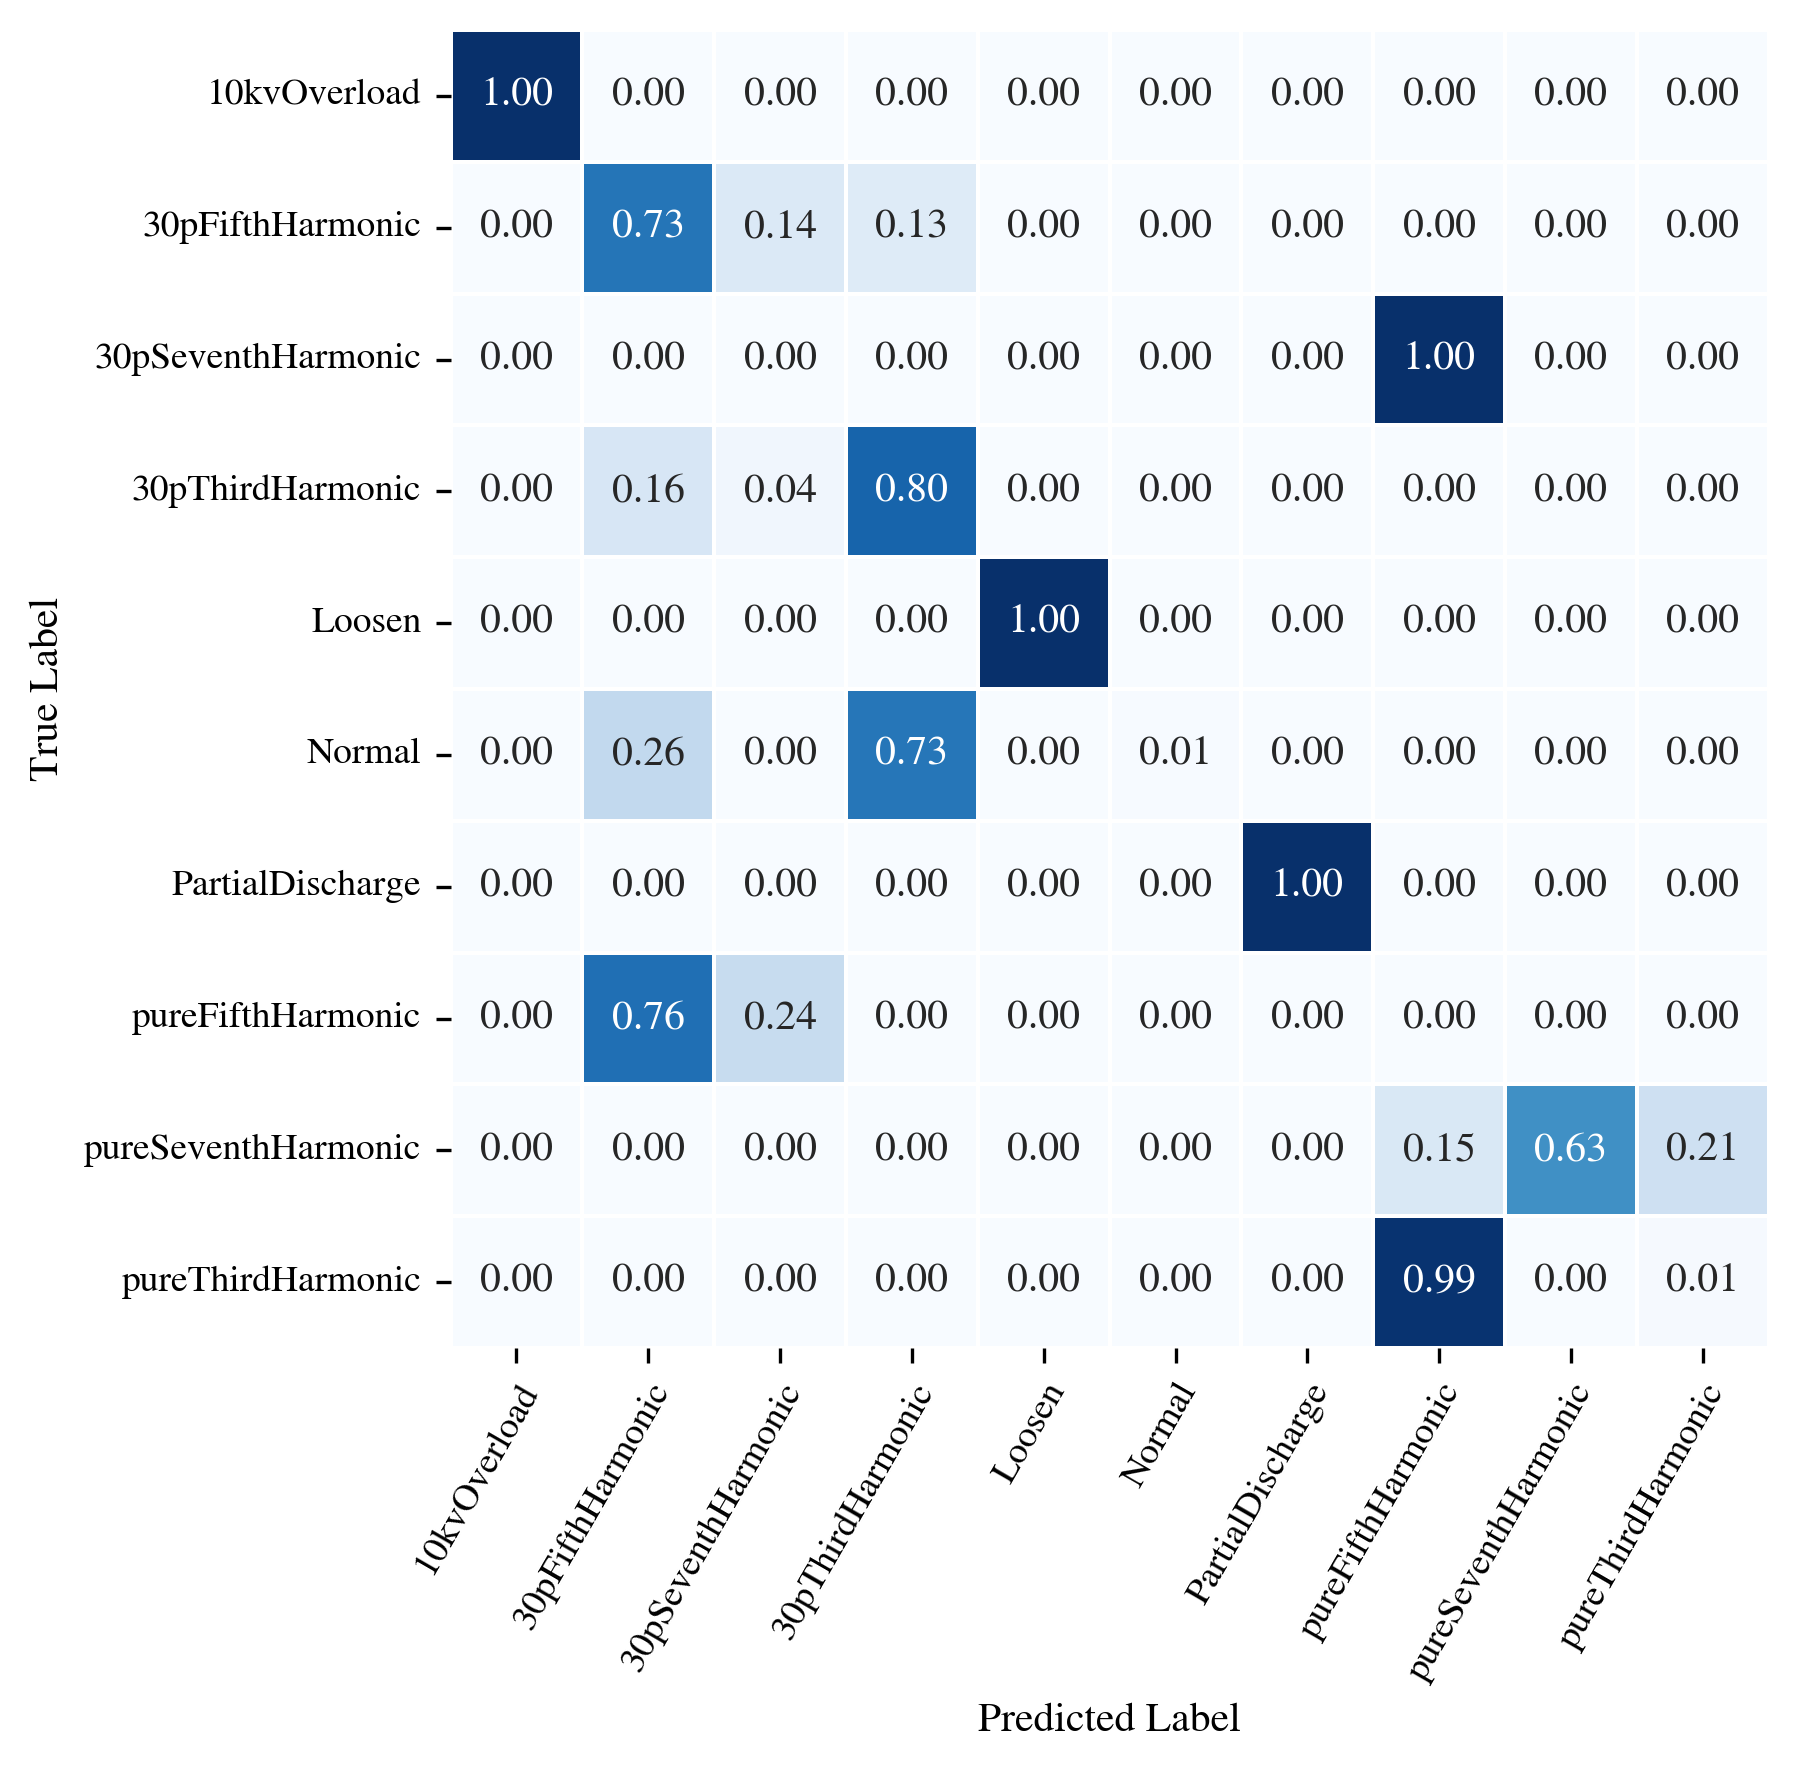
\includegraphics[width=\linewidth]{confusion_matrix/confusion_matrix_baseline}
			\caption{Baseline}
		\end{subfigure}
		\hfill
		\begin{subfigure}{0.48\textwidth}
			\centering
			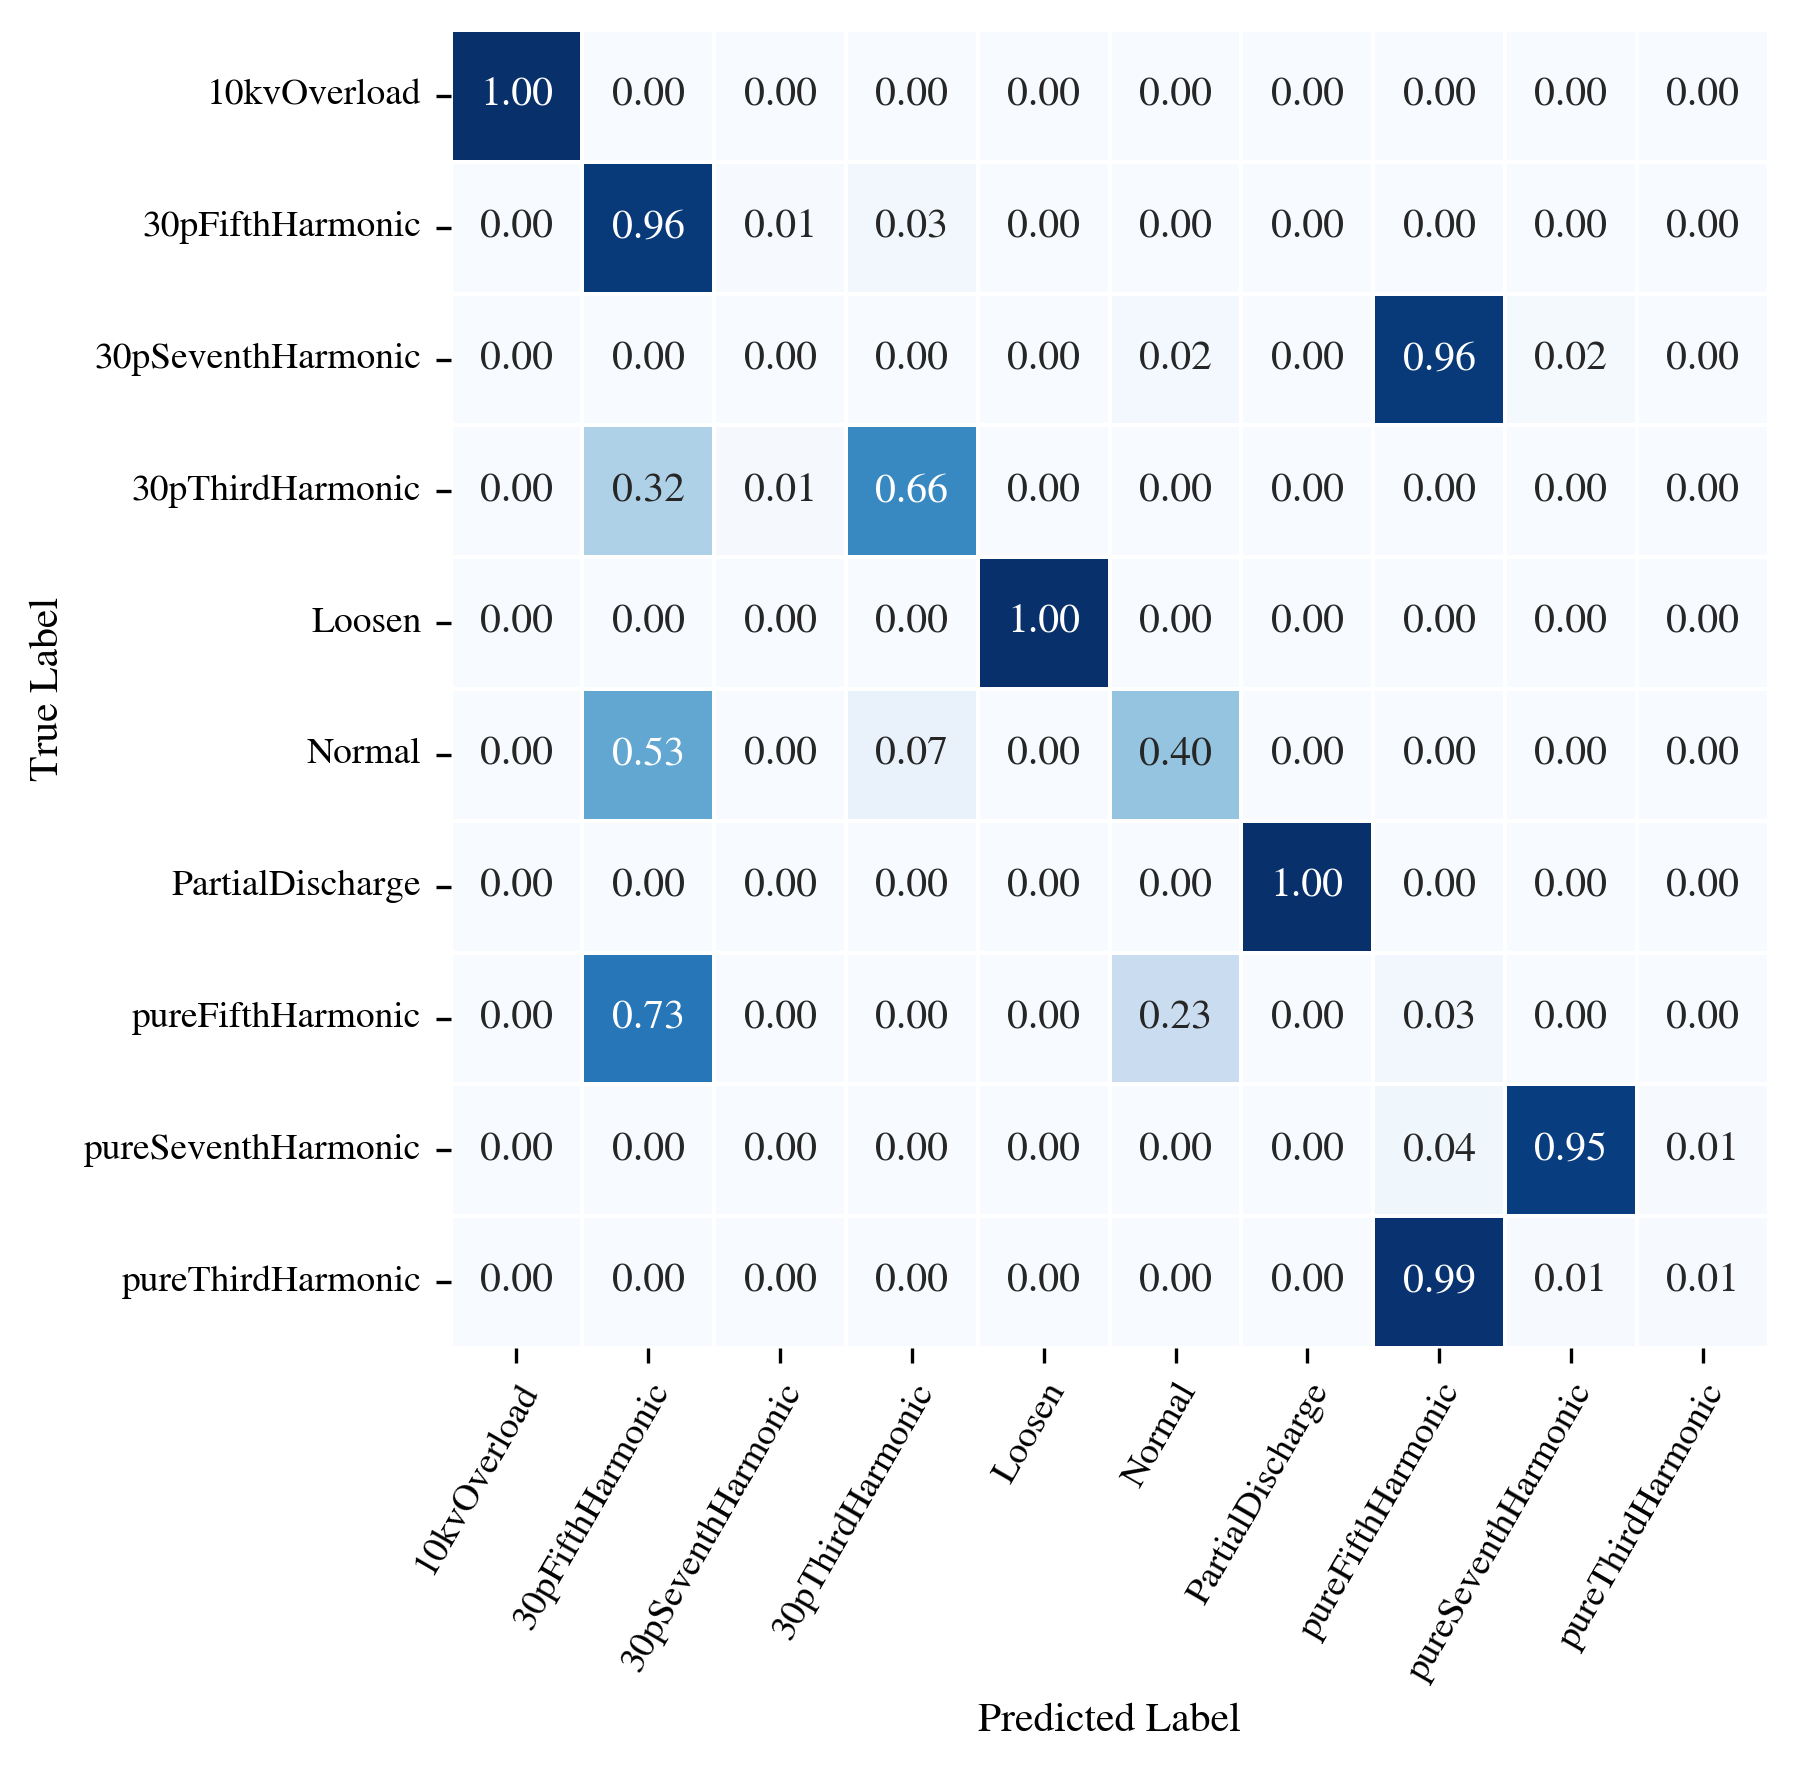
\includegraphics[width=\linewidth]{confusion_matrix/confusion_matrix_alexnet}
			\caption{AlexNet}
		\end{subfigure}\\[3mm]

		\begin{subfigure}{0.48\textwidth}
			\centering
			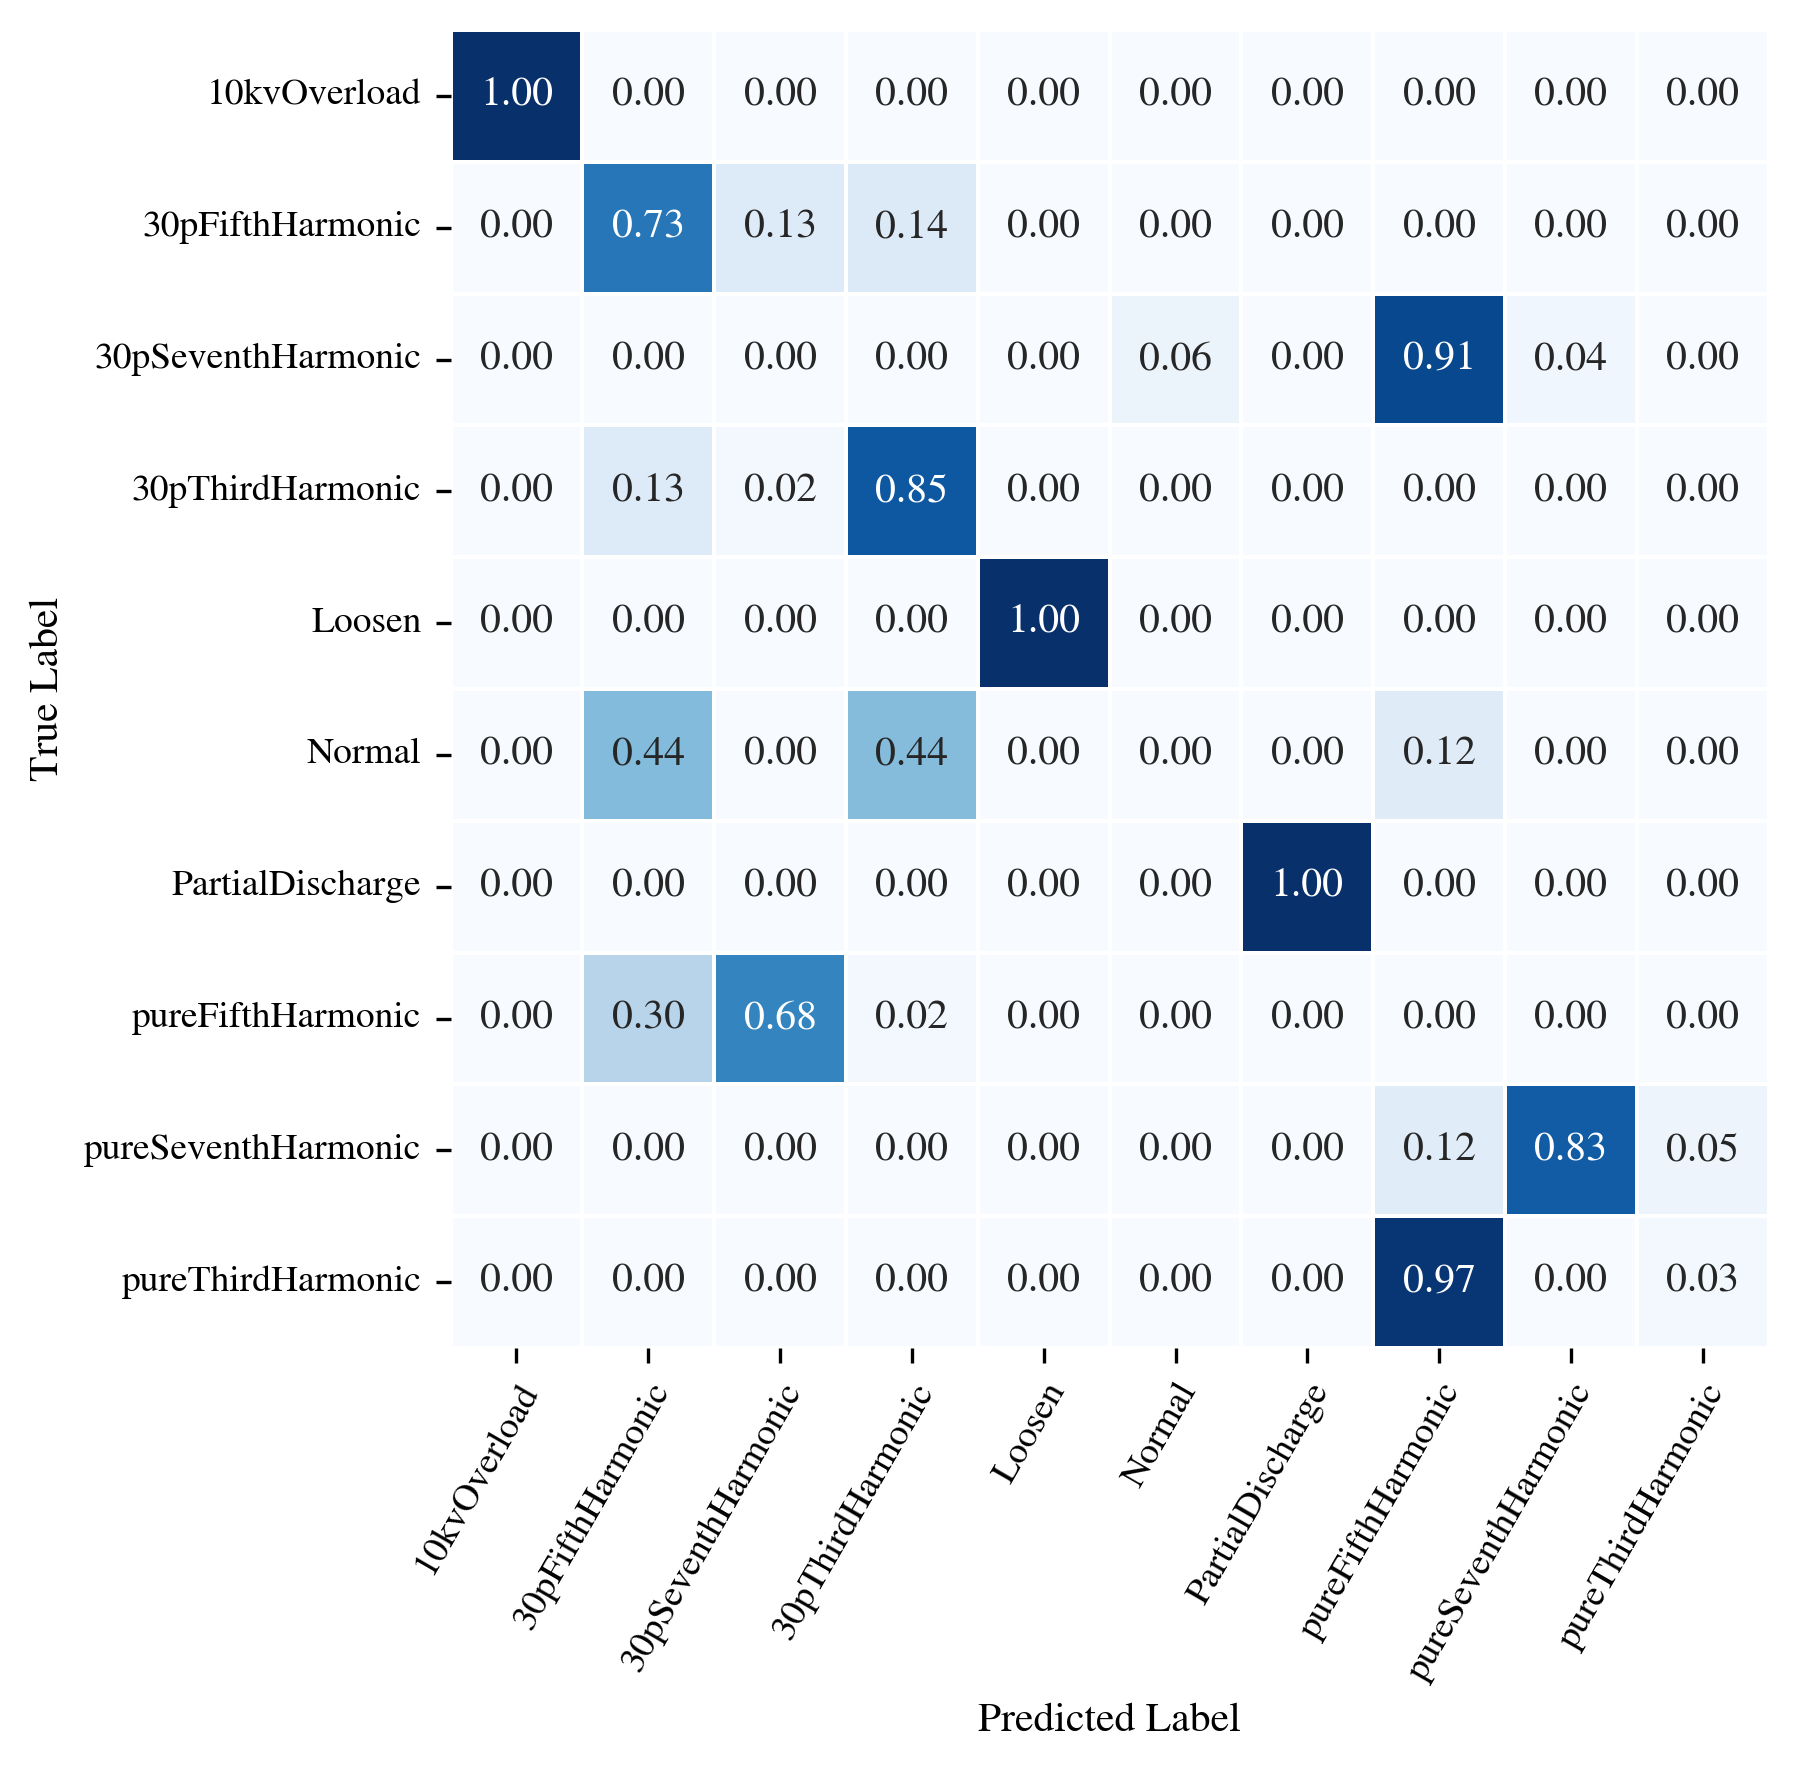
\includegraphics[width=\linewidth]{confusion_matrix/confusion_matrix_resnet18}
			\caption{ResNet18}
		\end{subfigure}
		\hfill
		\begin{subfigure}{0.48\textwidth}
			\centering
			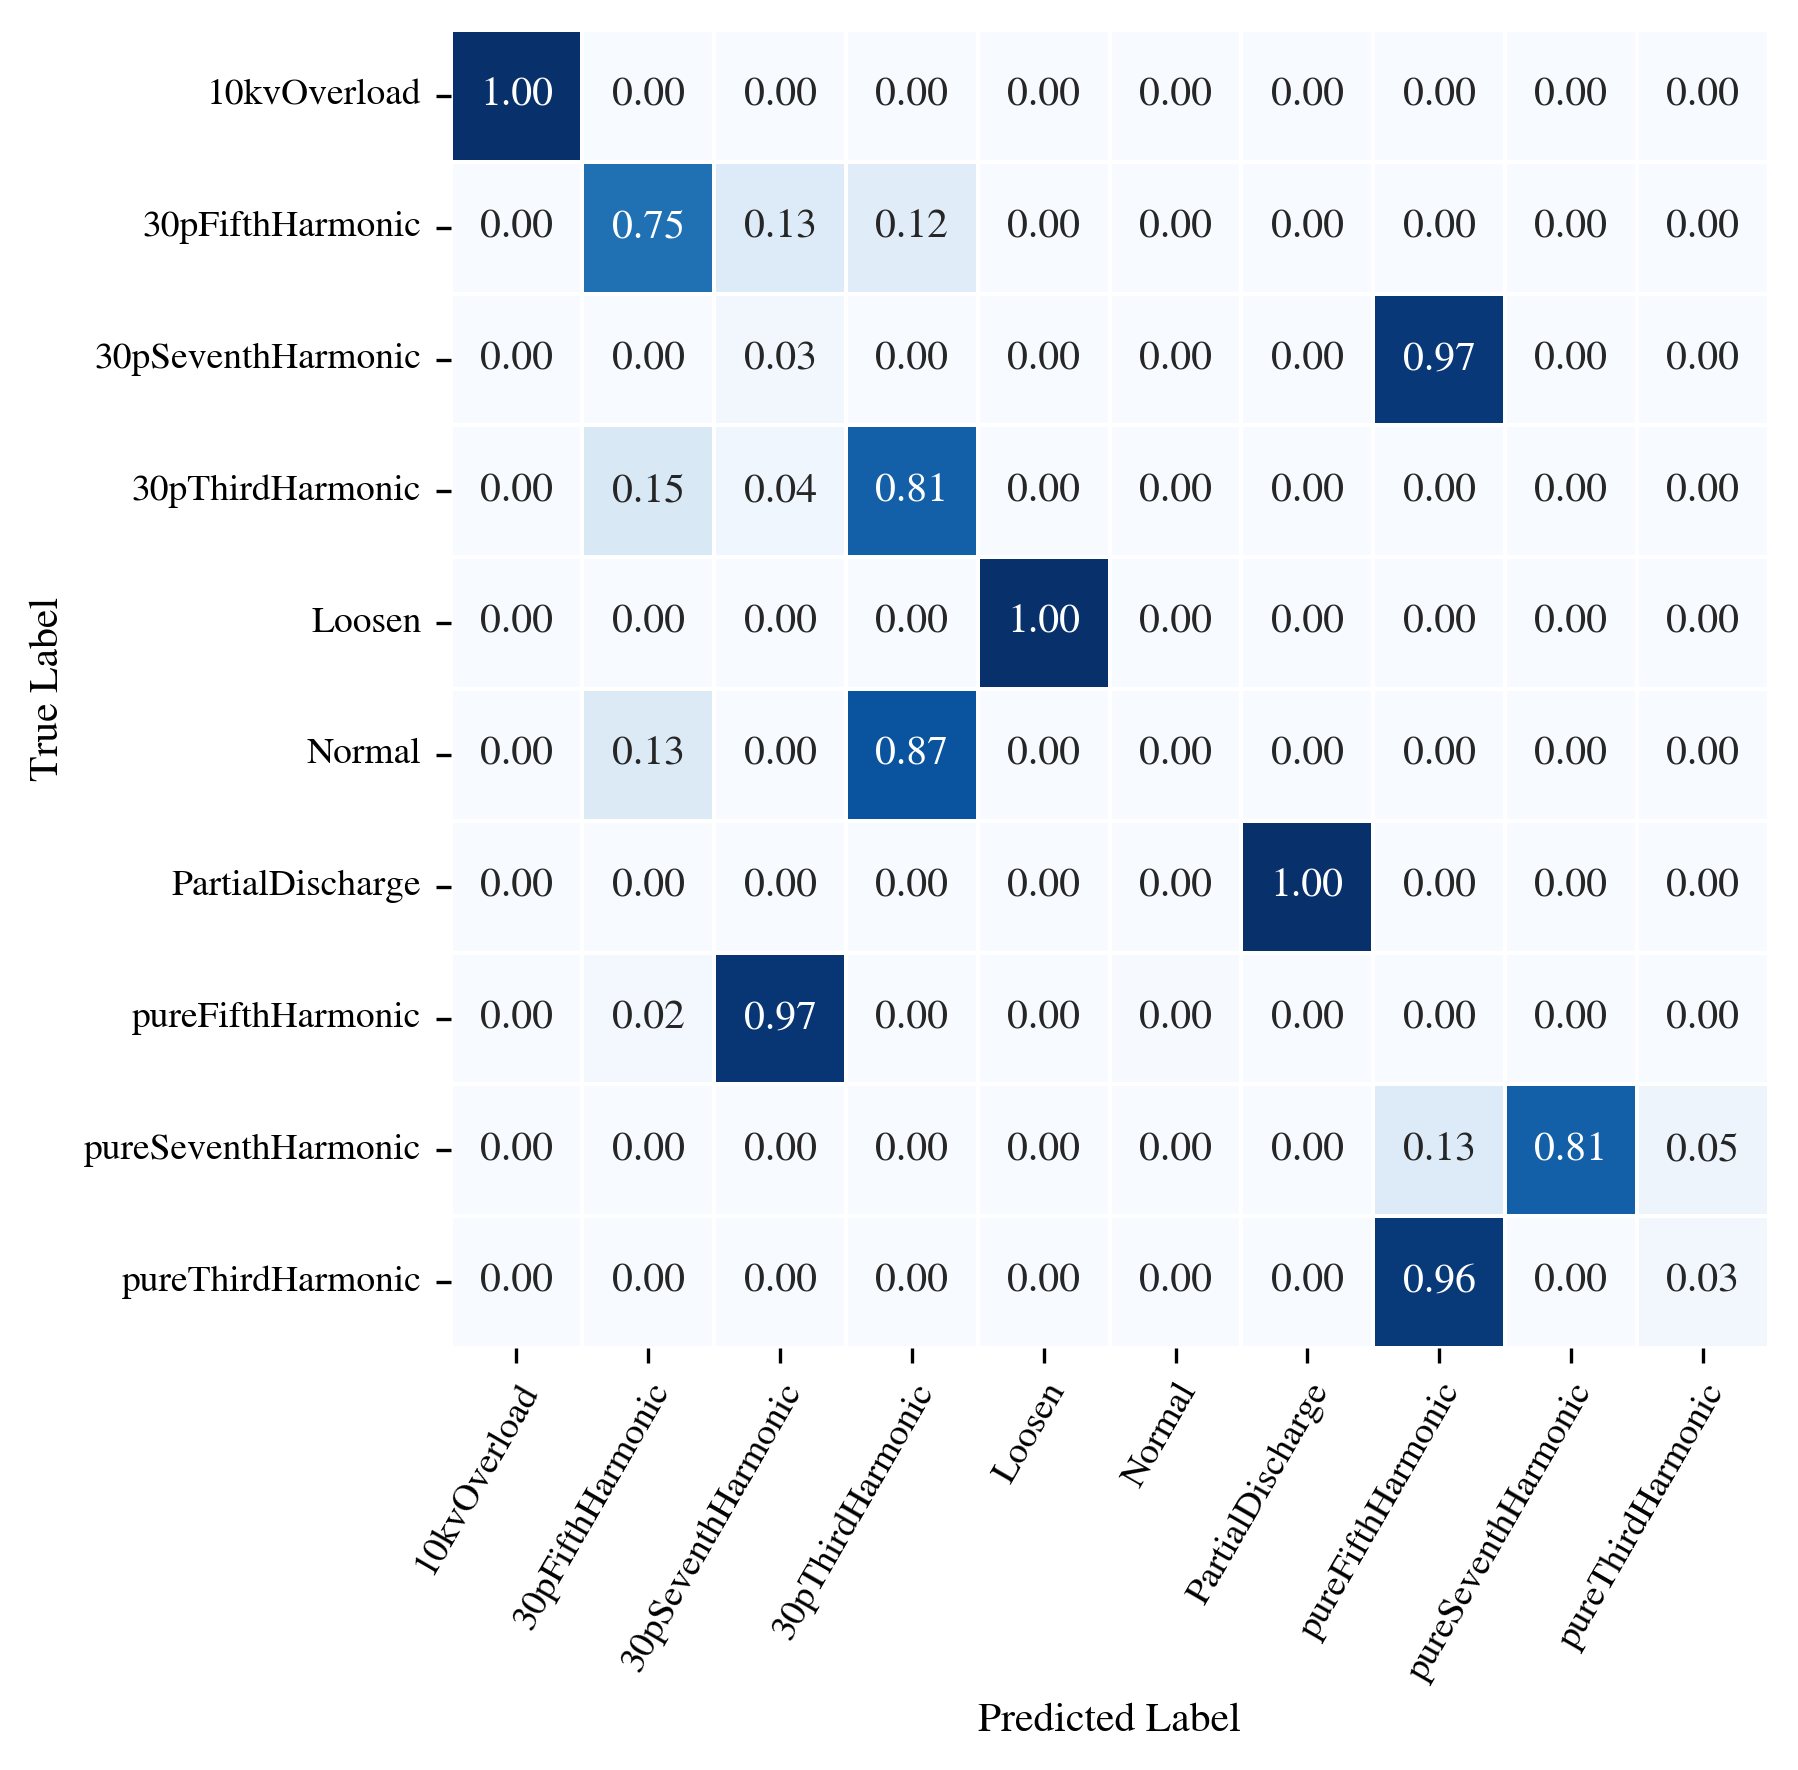
\includegraphics[width=\linewidth]{confusion_matrix/confusion_matrix_convnext_tiny}
			\caption{ConvNeXt-Tiny}
		\end{subfigure}\\[3mm]

		\begin{subfigure}{0.48\textwidth}
			\centering
			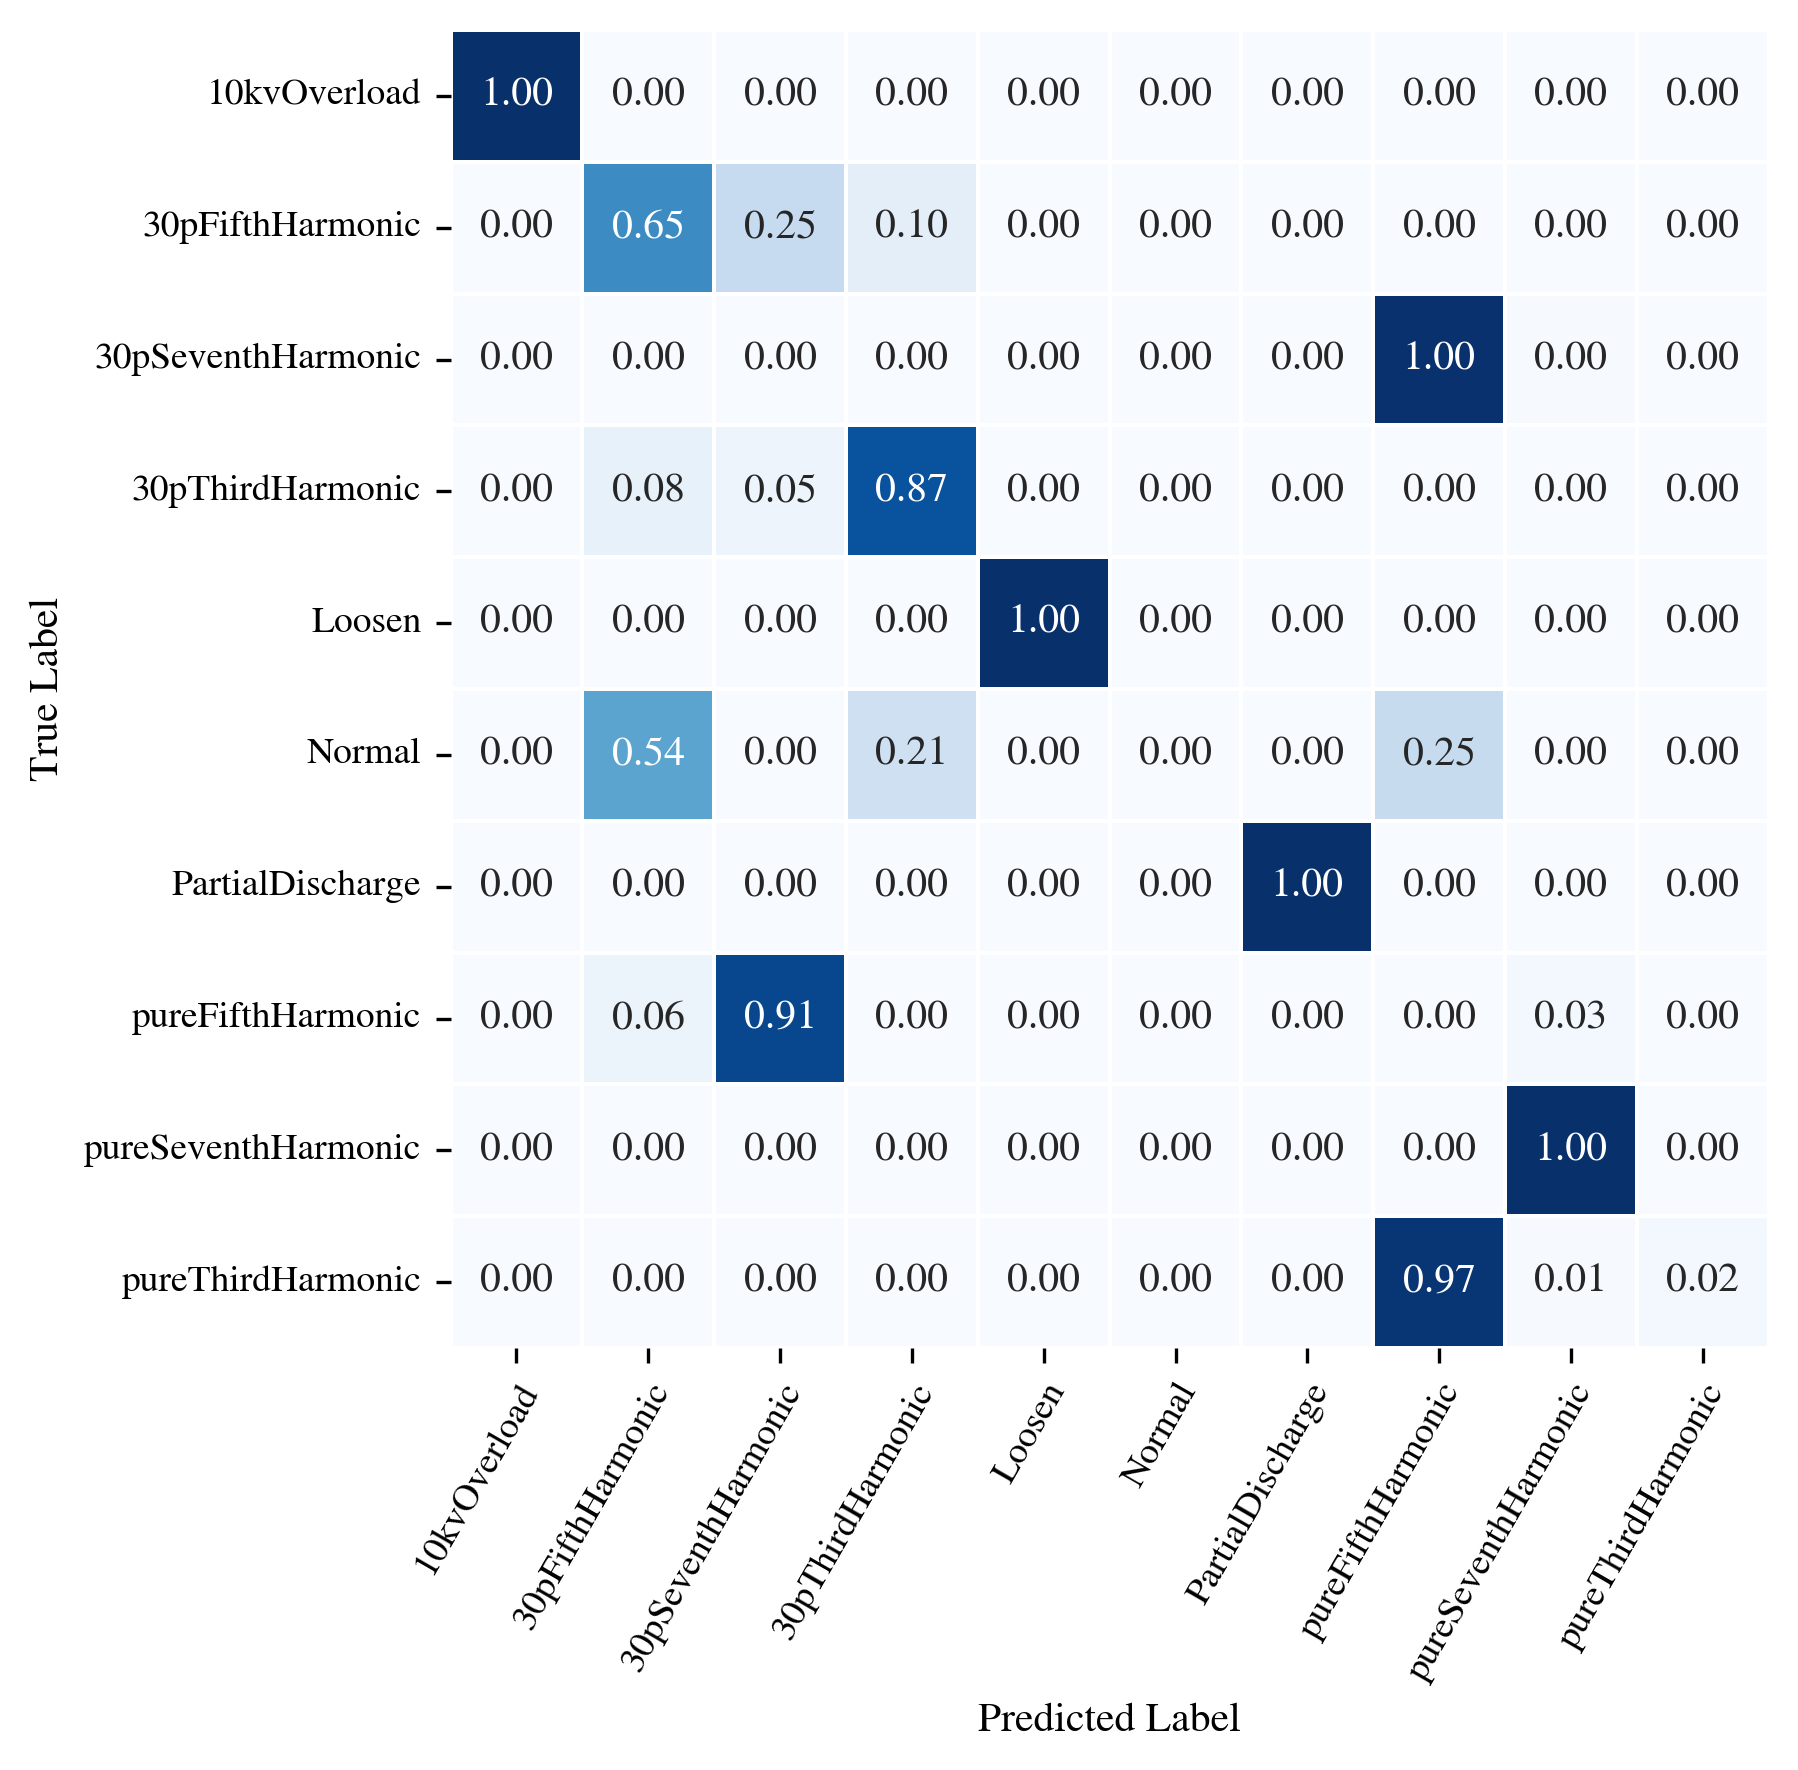
\includegraphics[width=\linewidth]{confusion_matrix/confusion_matrix_vgg16}
			\caption{VGG16}
		\end{subfigure}
		\hfill
		\begin{subfigure}{0.48\textwidth}
			\centering
			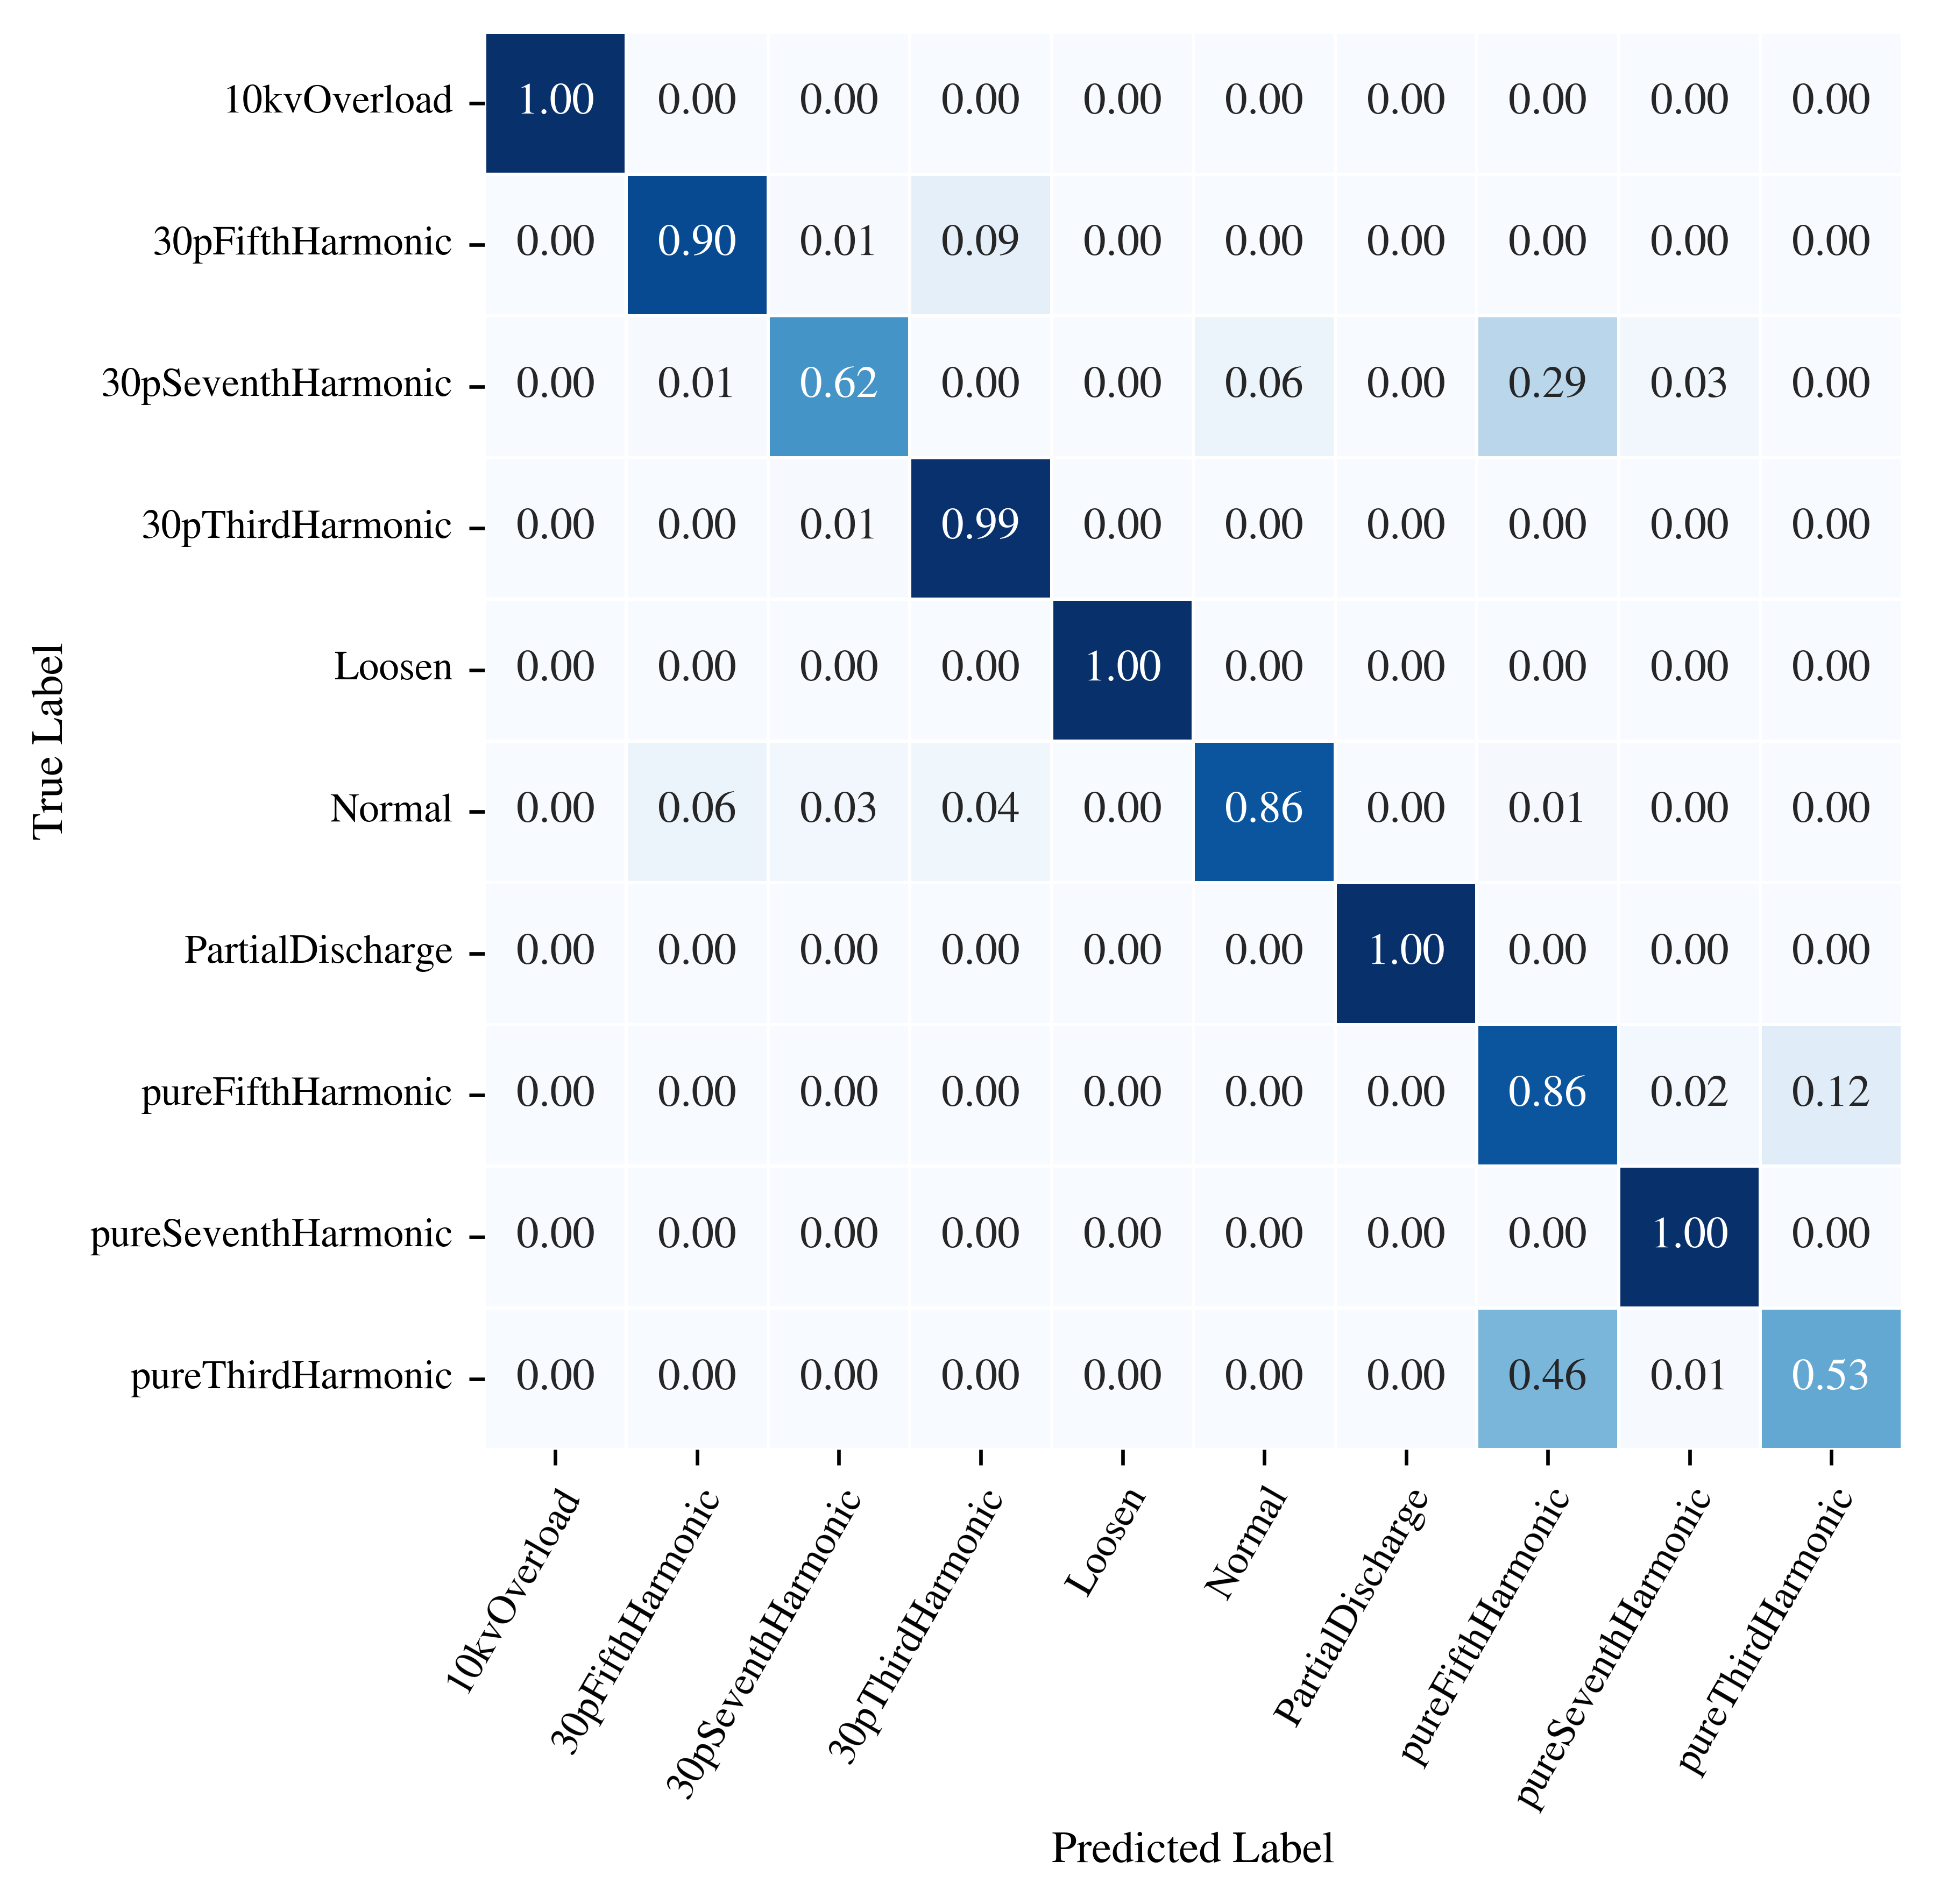
\includegraphics[width=\linewidth]{confusion_matrix/confusion_matrix__MSCA_VGG16}
			\caption{MSCA-VGG16 (Ours)}
		\end{subfigure}
		\caption{Confusion matrices of different network backbones trained using the AW-DPCNN fusion representations. The proposed MSCA-VGG16 achieves the most accurate classification performance with significantly reduced inter-class confusion.}
		\label{fig:confusion_matrix}
	\end{figure*}

\subsection{Backbone Comparison}
The key hyperparameters of the AW-DPCNN fusion module are summarized in Table~\ref{tab:awdpcnn_params}, where $\mathbf I$ denotes the identity matrix. Unless otherwise specified, these parameters remain fixed throughout all experiments to ensure fair comparison. The detailed configuration of the proposed MSCA-VGG16 network is summarized in Table~\ref{tab:msca_vgg16}, where $d_e$ denotes the dimension of the discriminative embedding.
\begin{table}
	\centering
	\caption{Key Hyperparameters of AW-DPCNN}
	\label{tab:awdpcnn_params}
	\begin{tabular}{ccc}
		\hline
		\textbf{Parameter} & \textbf{Symbol} & \textbf{Value} \\
		\hline
		Iteration number & $N$ & 20 \\
		Decay coefficient & $\alpha_L$ & 0.001 \\
		Threshold decay & $\alpha_T$ & 0.001 \\
		Amplification coefficient & $V_T$ & 20 \\
		Stabilization constant & $\sigma$ & 0.1 \\
		Contrast amplification factor & $\gamma$ & 4 \\
		Local neighborhood window size & $\boldsymbol{\Omega}$ & $3 \times 3$ \\
		Kernel size of Mel channel & $\boldsymbol{W}_1$ & $3 \times 5$ \\
		Kernel size of GADF channel & $\boldsymbol{W}_2$ & $3 \times 3$ \\
		Coupling matrix & $\boldsymbol{M}$ & $$0.25\,I$$ \\
		\hline
	\end{tabular}
\end{table}
\begin{table}
	\centering
	\caption{Configuration of the Proposed MSCA-VGG16 Network}
	\begin{tabular}{lcccc}
		\toprule
		\textbf{Type} & \textbf{Layer} & \textbf{Kernel / Operation} & \textbf{Input Size} & \textbf{Output Size} \\
		\midrule
		Input & AW-DPCNN fused image & None & $224 \times 224 \times 3$ & $224 \times 224 \times 3$ \\
		Feature Extractor & VGG16 convolution blocks & $3\times3$ conv + max pooling & $224 \times 224 \times 3$ & $7 \times 7 \times 512$ \\
		MSCA Module & Multi-scale conv + SE attention & $3\times3$, $5\times5$, dilated conv & $7 \times 7 \times 512$ & $7 \times 7 \times 512$ \\
		Pooling & Global average pooling & $7\times7$ & $7 \times 7 \times 512$ & $1 \times 1 \times 512$ \\
		FC Layer & Fully connected & 512 $\rightarrow$ 4096 & 512 & 4096 \\
		Embedding & Discriminative embedding & $4096 \rightarrow d_e$ & 4096 & $d_e$ \\
		Classifier & Softmax output & $d_e \rightarrow 10$ & $d_e$ & 10 \\
		\bottomrule
	\end{tabular}
	\label{tab:msca_vgg16}
\end{table}



To evaluate the effectiveness of the proposed classification network, a comparative experiment was conducted using several representative deep learning backbones, including Baseline CNN, AlexNet, ResNet18, ConvNeXt-Tiny, and VGG16. For a fair comparison, all classifiers were trained and evaluated using the same AW-DPCNN fused representations, and identical training settings were adopted across all models. It can be observed from Table~\ref{tab:network_comparison} that different backbone networks exhibit varying performance in transformer fault classification. The baseline model achieves relatively limited results, with an accuracy of 73.31\% and an F1-score of 69.59\%. By adopting deeper architectures such as AlexNet, ResNet18, ConvNeXt-Tiny, and VGG16, the classification performance improves to different extents, indicating that more powerful feature extraction networks can better capture discriminative acoustic characteristics. Among all compared methods, the proposed MSCA-VGG16 achieves the best performance across all evaluation metrics. Specifically, it obtains an accuracy of 87.45\%, an F1-score of 86.97\%, and a G-mean of 85.69\%, which are significantly higher than those of the other backbone models. Compared with the baseline model, the accuracy improves by more than 14\%. Moreover, the balanced accuracy and Kappa coefficient reach 87.50\% and 86.03\%, respectively, indicating improved classification consistency and robustness across different fault categories. These results demonstrate the effectiveness of the proposed MSCA-VGG16 framework for transformer acoustic fault diagnosis.
\begin{table}
	\centering
	\caption{Performance Comparison with Different Backbone Networks}
	\label{tab:network_comparison}
	\begin{tabular}{lcccccc}
		\toprule
		\textbf{Network} 
		& \textbf{Acc (\%)} 
		& \textbf{Recall (\%)} 
		& \textbf{F1 (\%)} 
		& \textbf{G-mean (\%)} 
		& \textbf{B-Acc (\%)} 
		& \textbf{Kappa (\%)} \\
		\midrule
		Baseline &73.31 &74.23 &69.59 &42.47 &74.23 &70.41 \\
		AlexNet &79.97 &81.94 &77.31 &52.96 &81.94 &77.79 \\
		ResNet18 &79.18 &81.00 &76.69 &52.37 &81.00 &76.91 \\
		ConvNeXt-Tiny &79.82 &81.27 &78.28 &70.81 &81.27 &77.61 \\
		VGG16 &78.15 &79.68 &75.82 &57.37 &79.68 &75.76 \\
		\textbf{MSCA-VGG16 (Ours)} 
		& \textbf{87.45} & \textbf{87.50} 
		& \textbf{86.97} & \textbf{85.69} 
		& \textbf{87.50} & \textbf{86.03} \\
		\bottomrule
	\end{tabular}
\end{table}




% \begin{figure*}[!t]
% 	\centering
% 	\begin{subfigure}{0.32\textwidth}
% 		\centering
% 		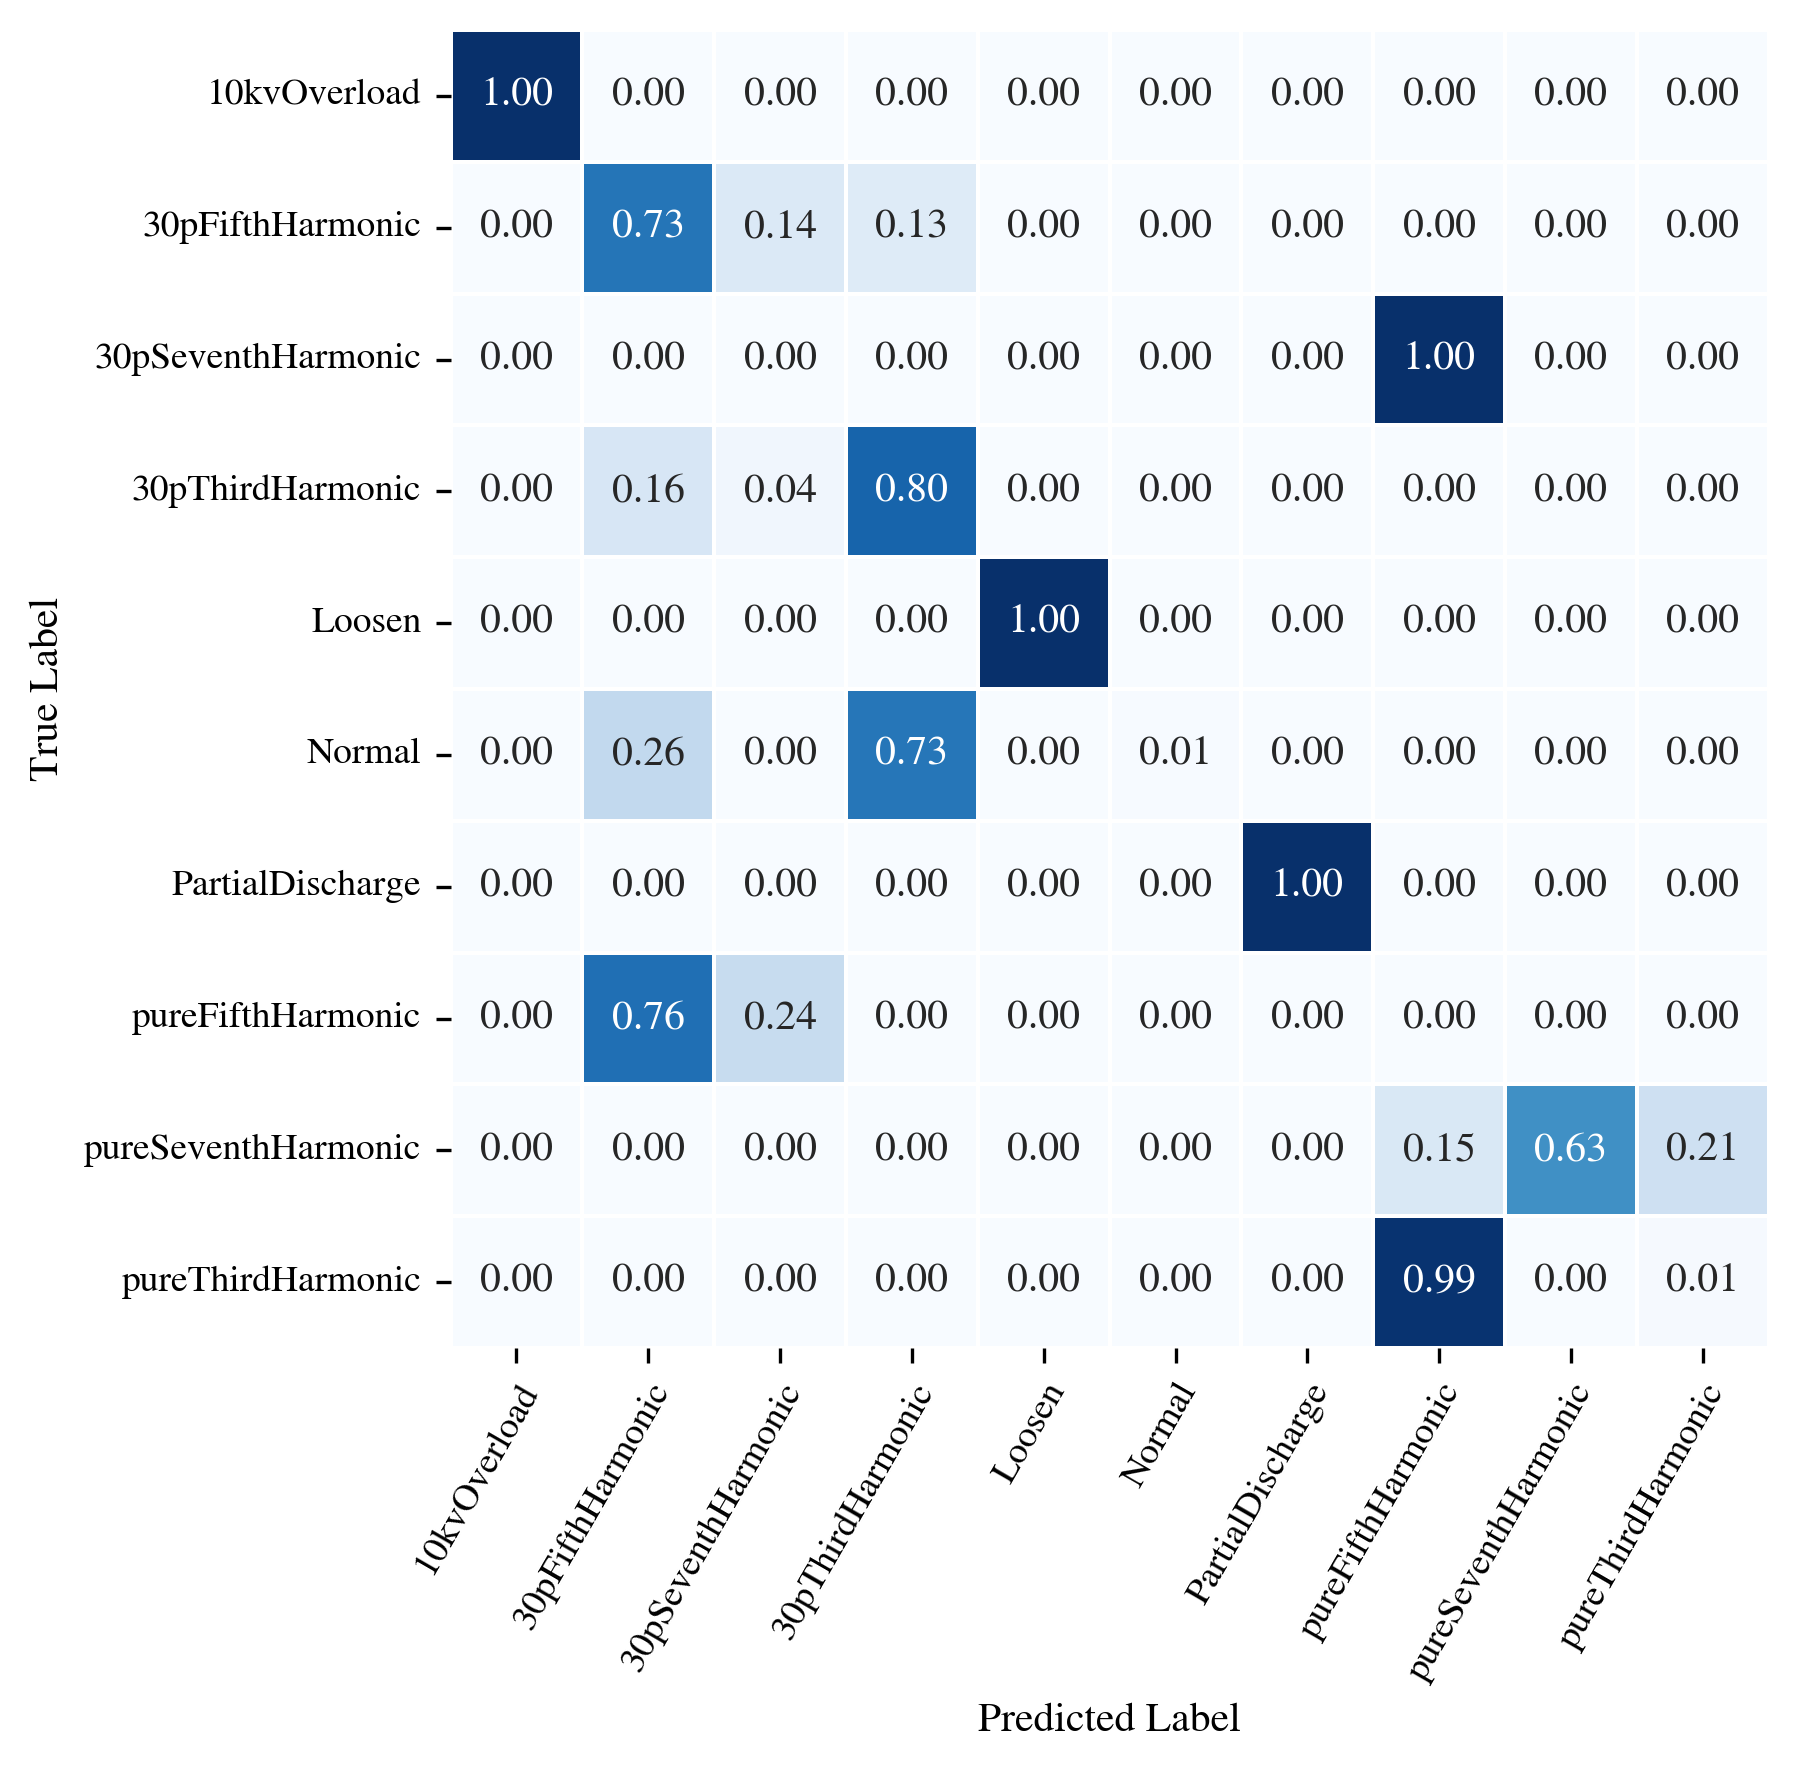
\includegraphics[width=\linewidth]{confusion_matrix/confusion_matrix_baseline}
% 		\caption{Baseline}
% 	\end{subfigure}
% 	\hfill
% 	\begin{subfigure}{0.32\textwidth}
% 		\centering
% 		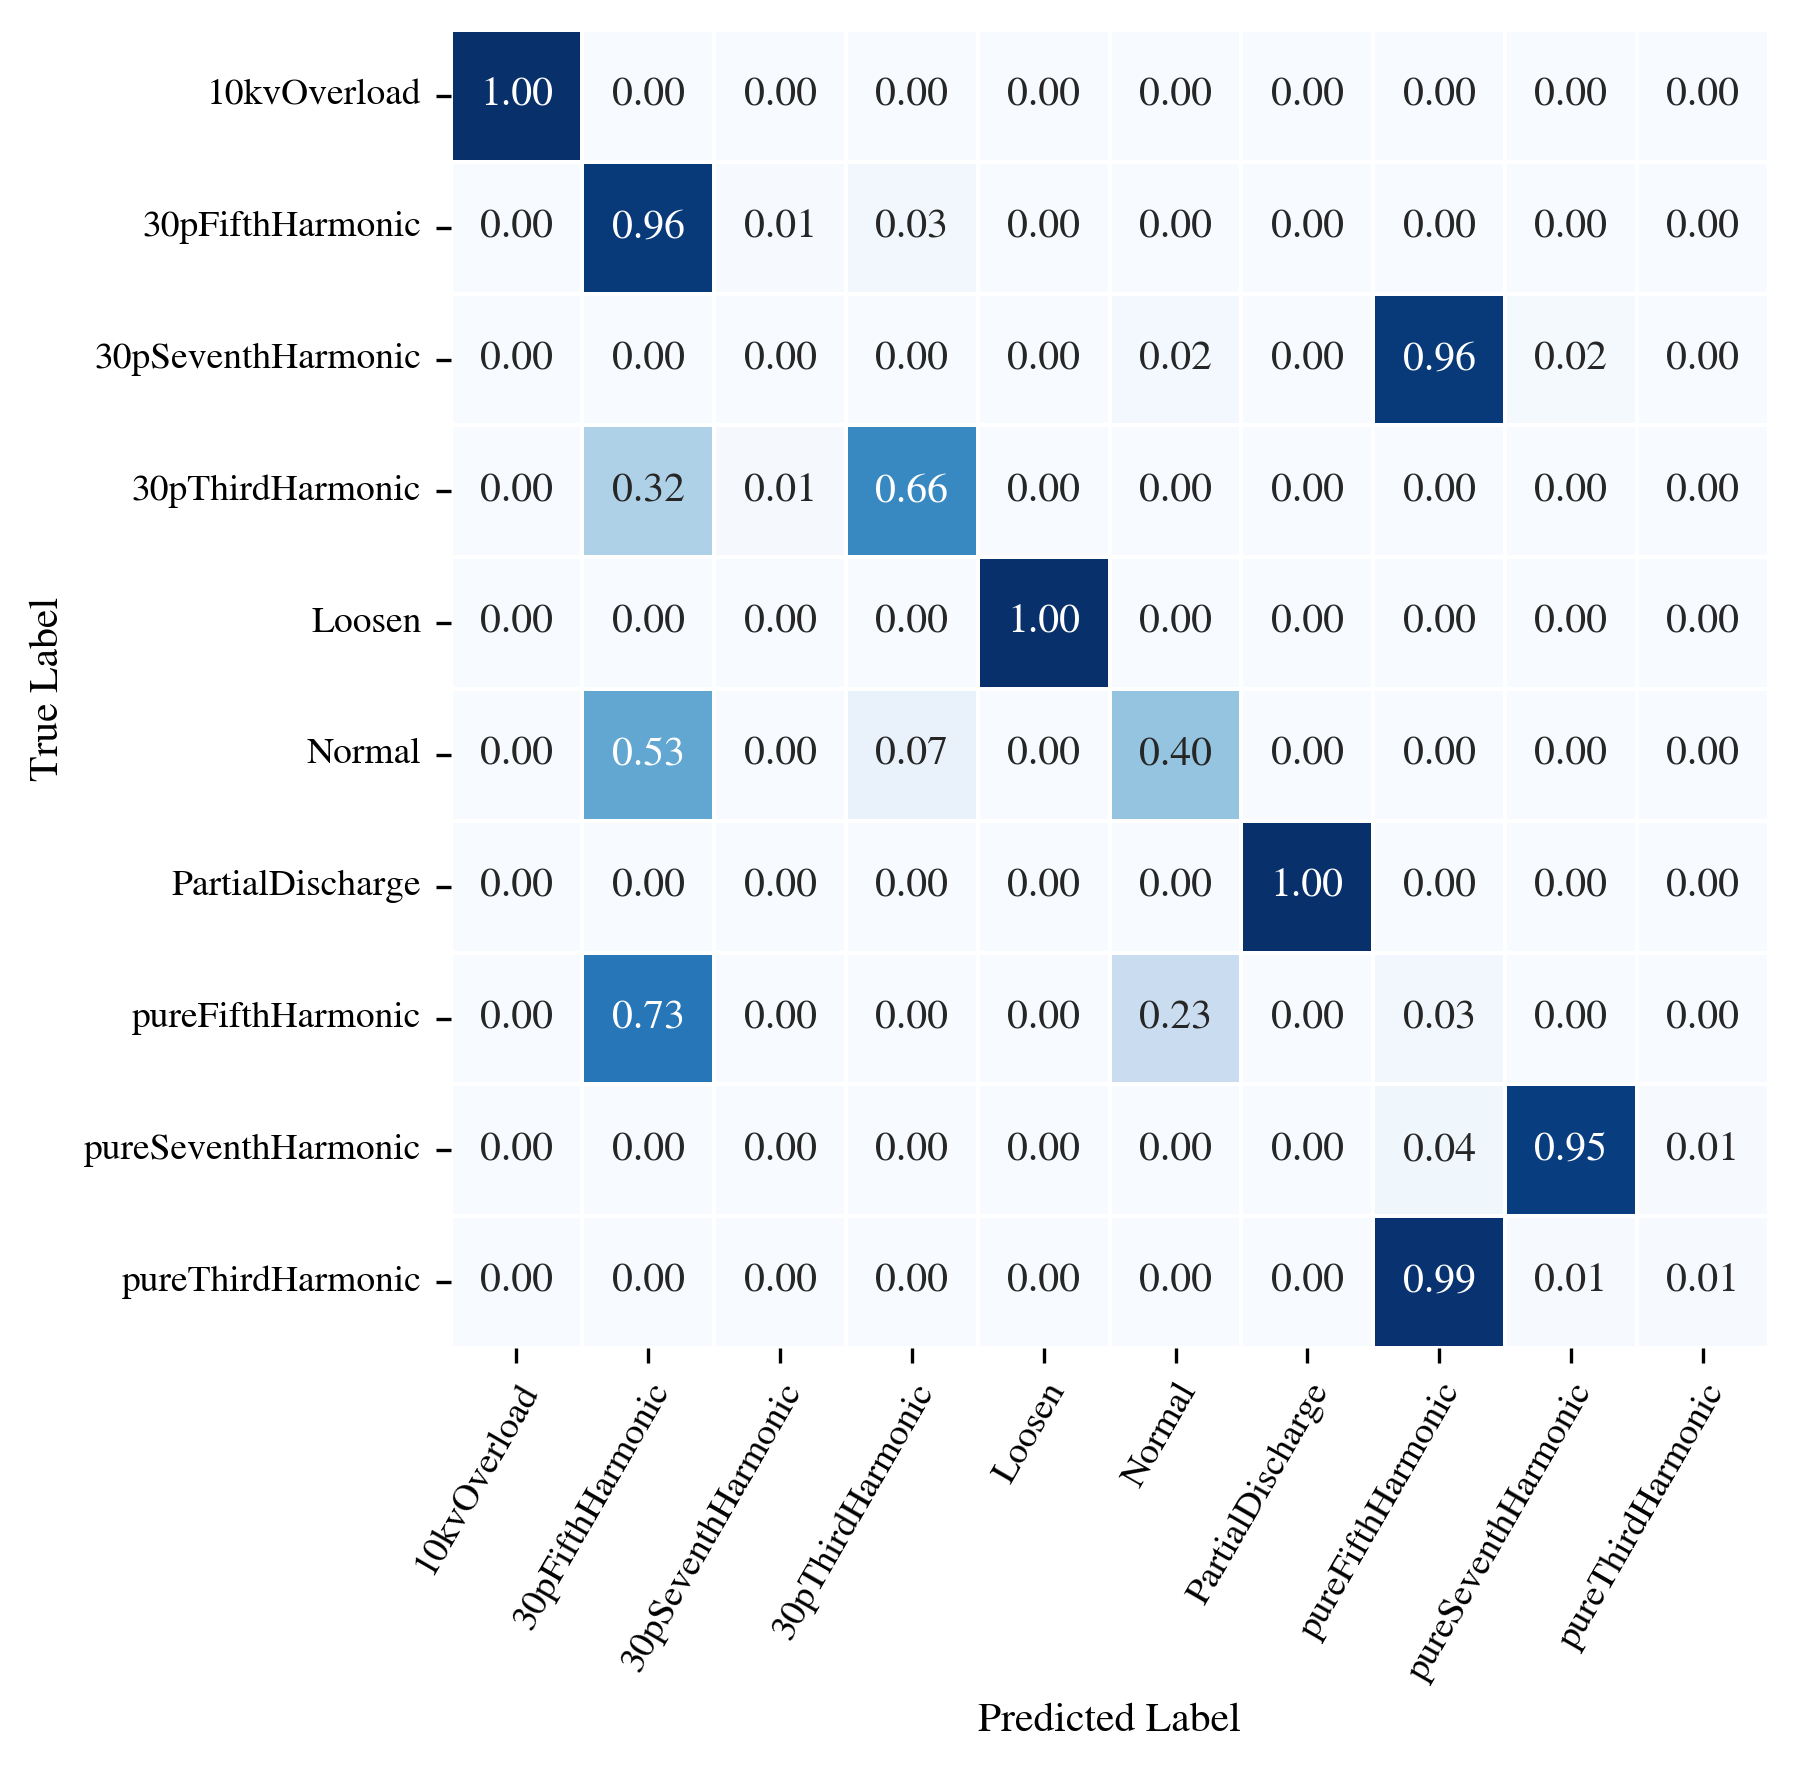
\includegraphics[width=\linewidth]{confusion_matrix/confusion_matrix_alexnet}
% 		\caption{AlexNet}
% 	\end{subfigure}
% 	\hfill
% 	\begin{subfigure}{0.32\textwidth}
% 		\centering
% 		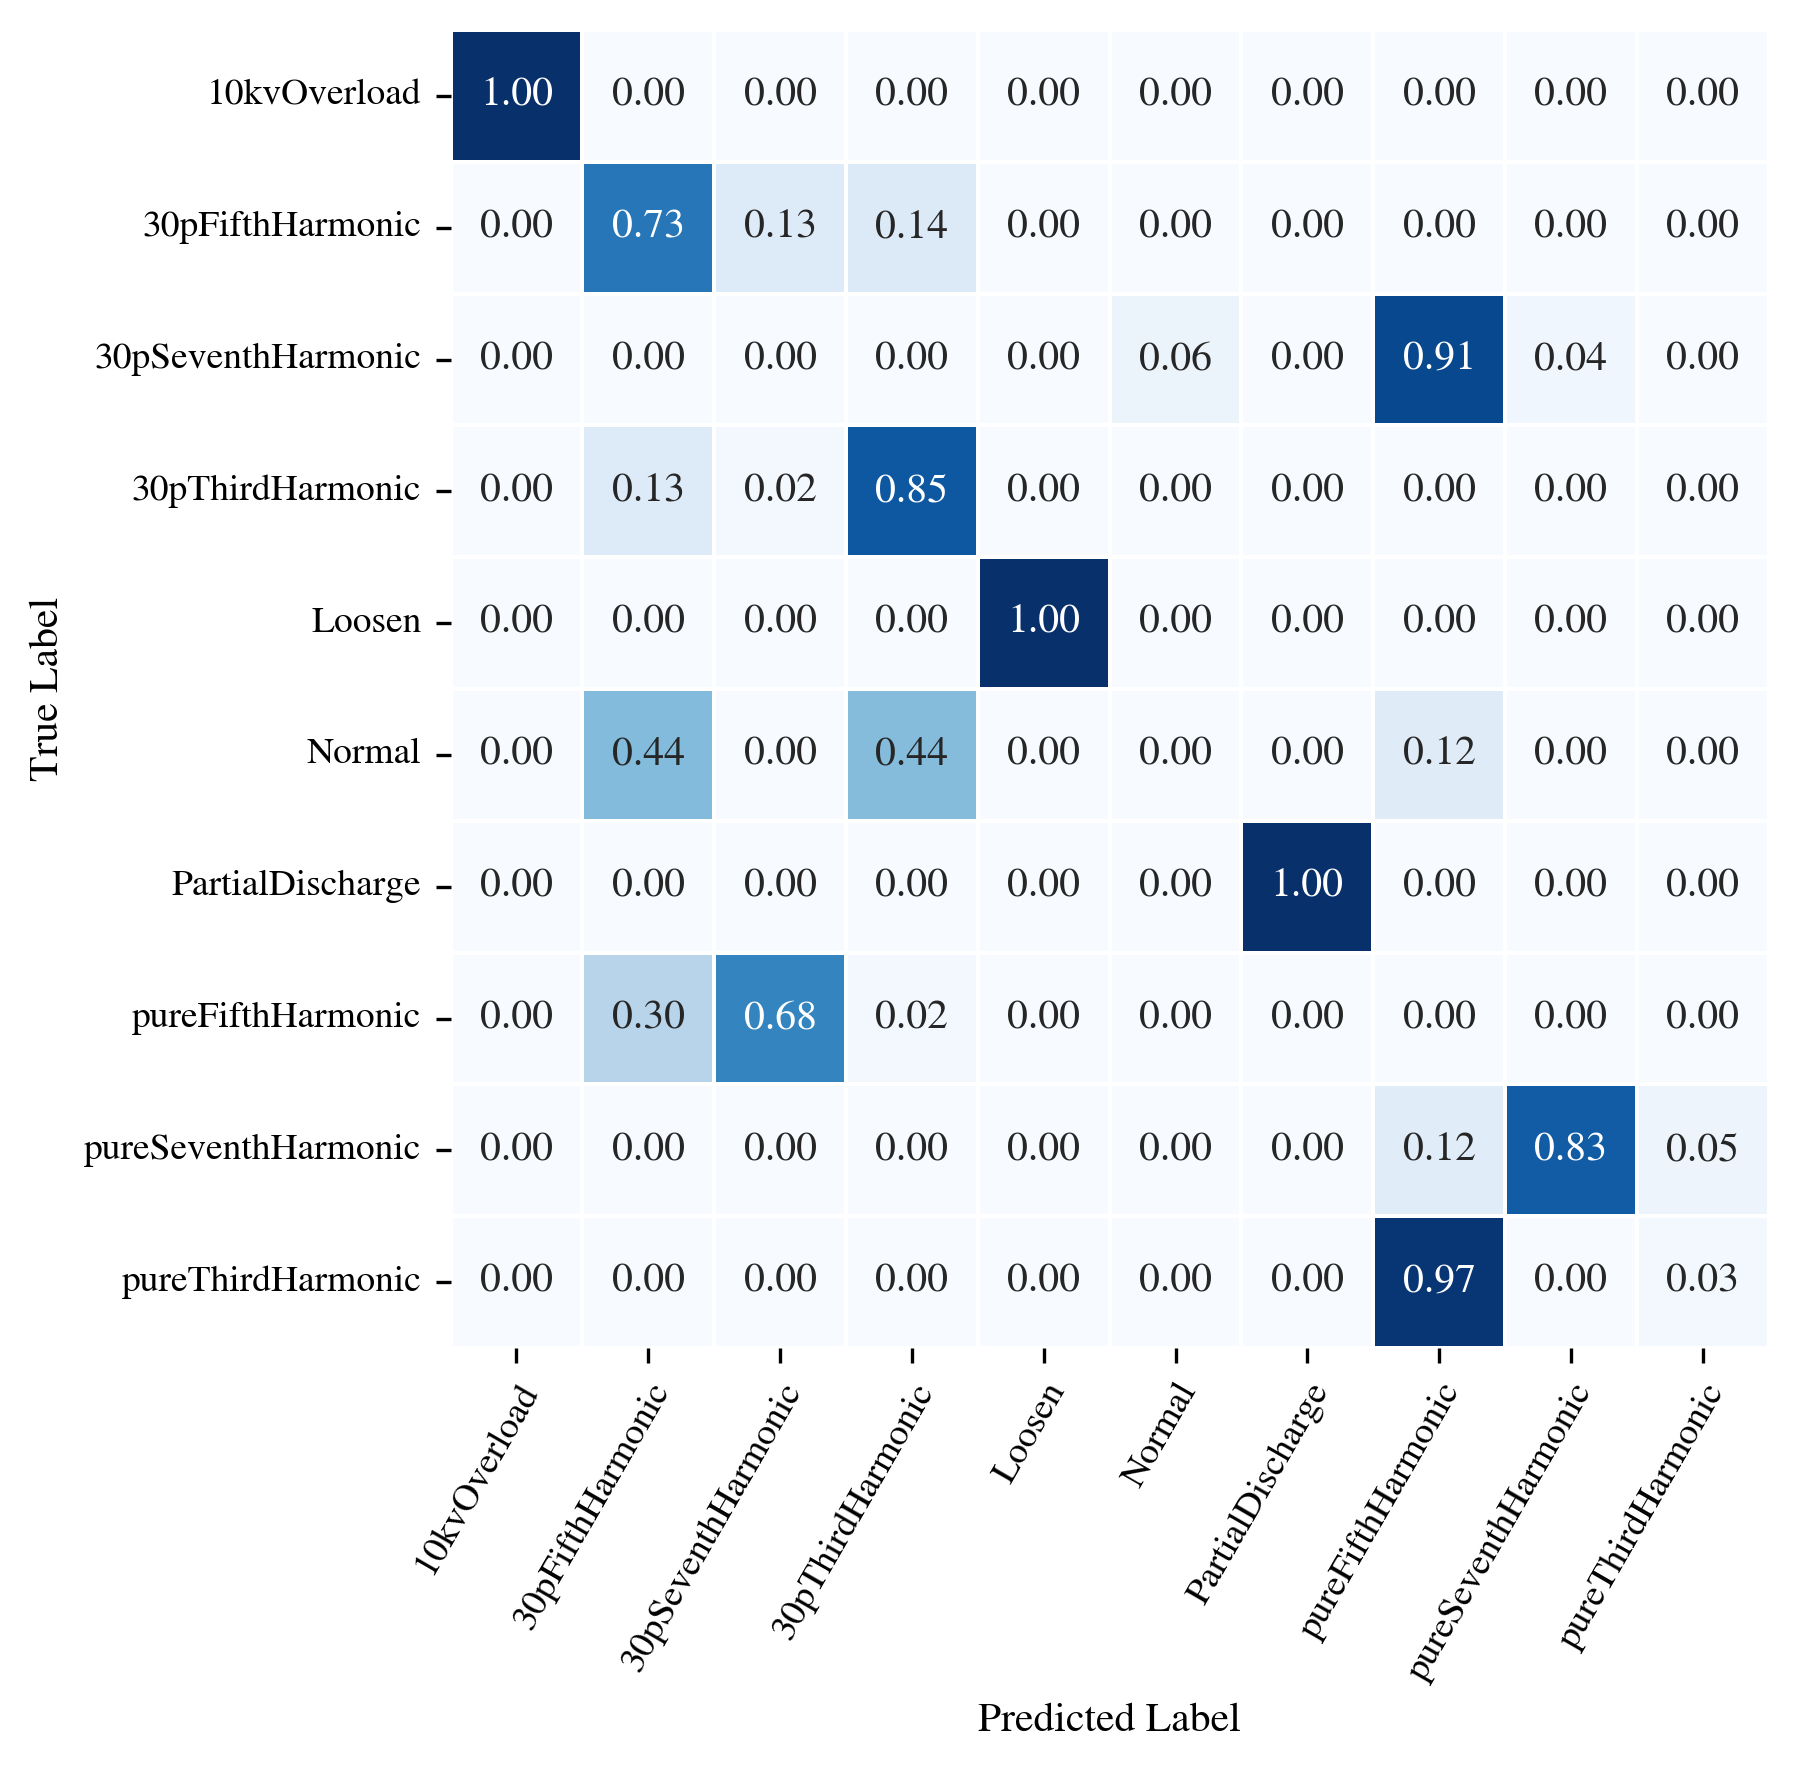
\includegraphics[width=\linewidth]{confusion_matrix/confusion_matrix_resnet18}
% 		\caption{ResNet18}
% 	\end{subfigure}
% 	\vspace{3mm}
% 	\begin{subfigure}{0.32\textwidth}
% 		\centering
% 		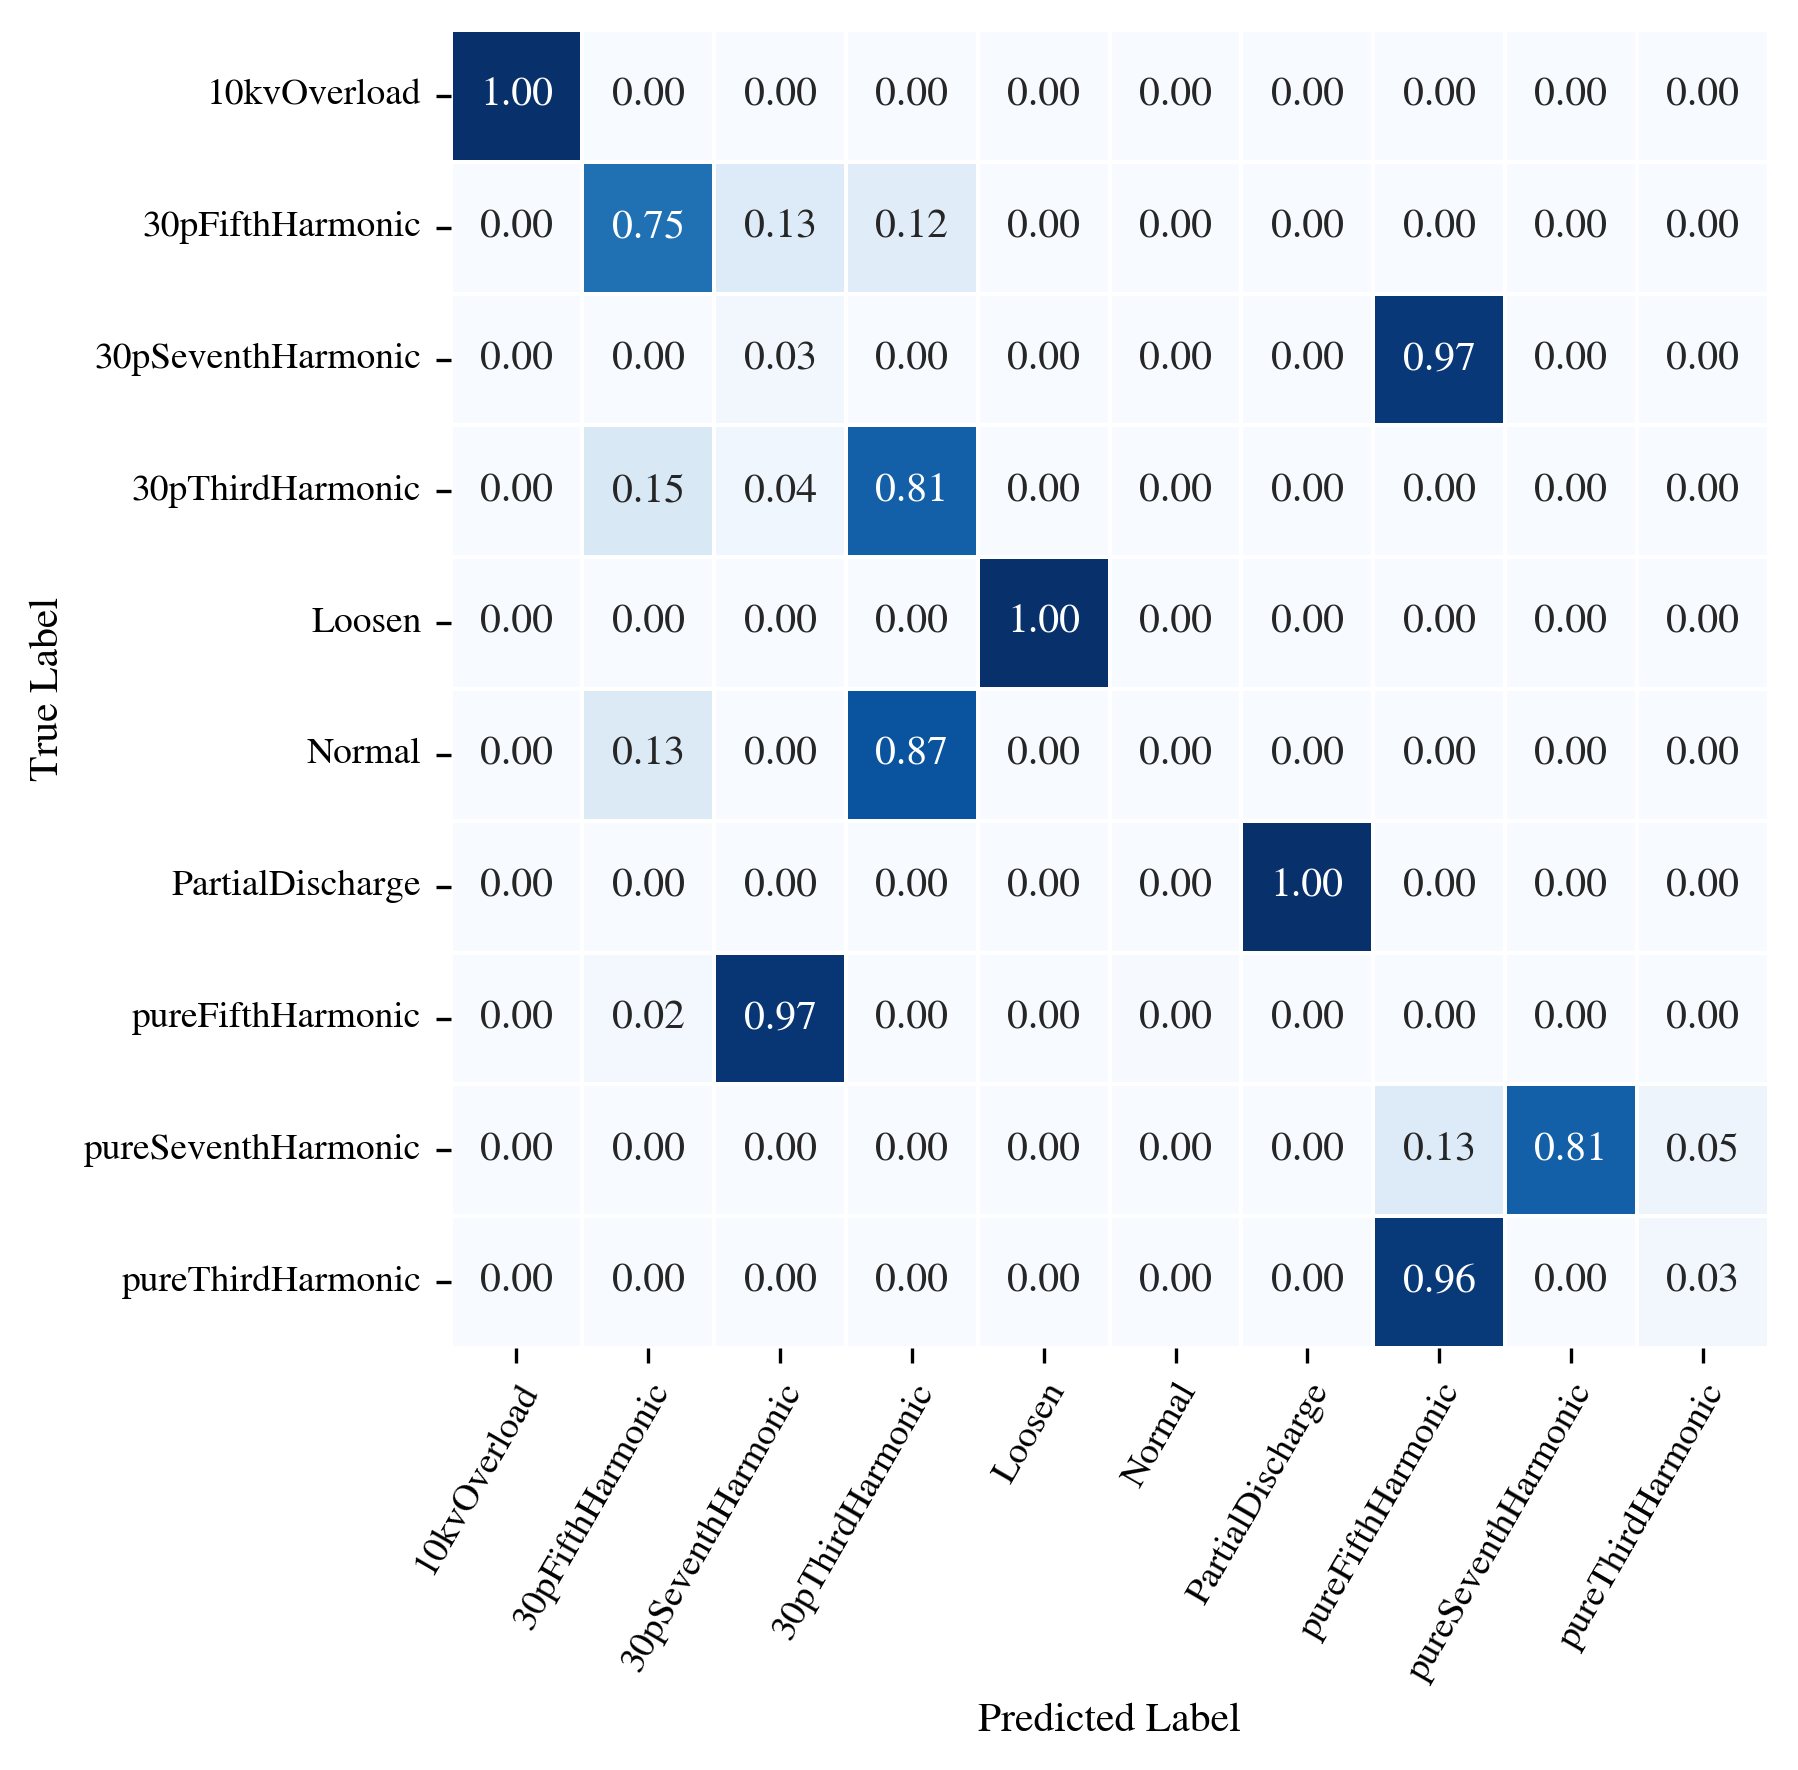
\includegraphics[width=\linewidth]{confusion_matrix/confusion_matrix_convnext_tiny}
% 		\caption{ConvNeXt-Tiny}
% 	\end{subfigure}
% 	\hfill
% 	\begin{subfigure}{0.32\textwidth}
% 		\centering
% 		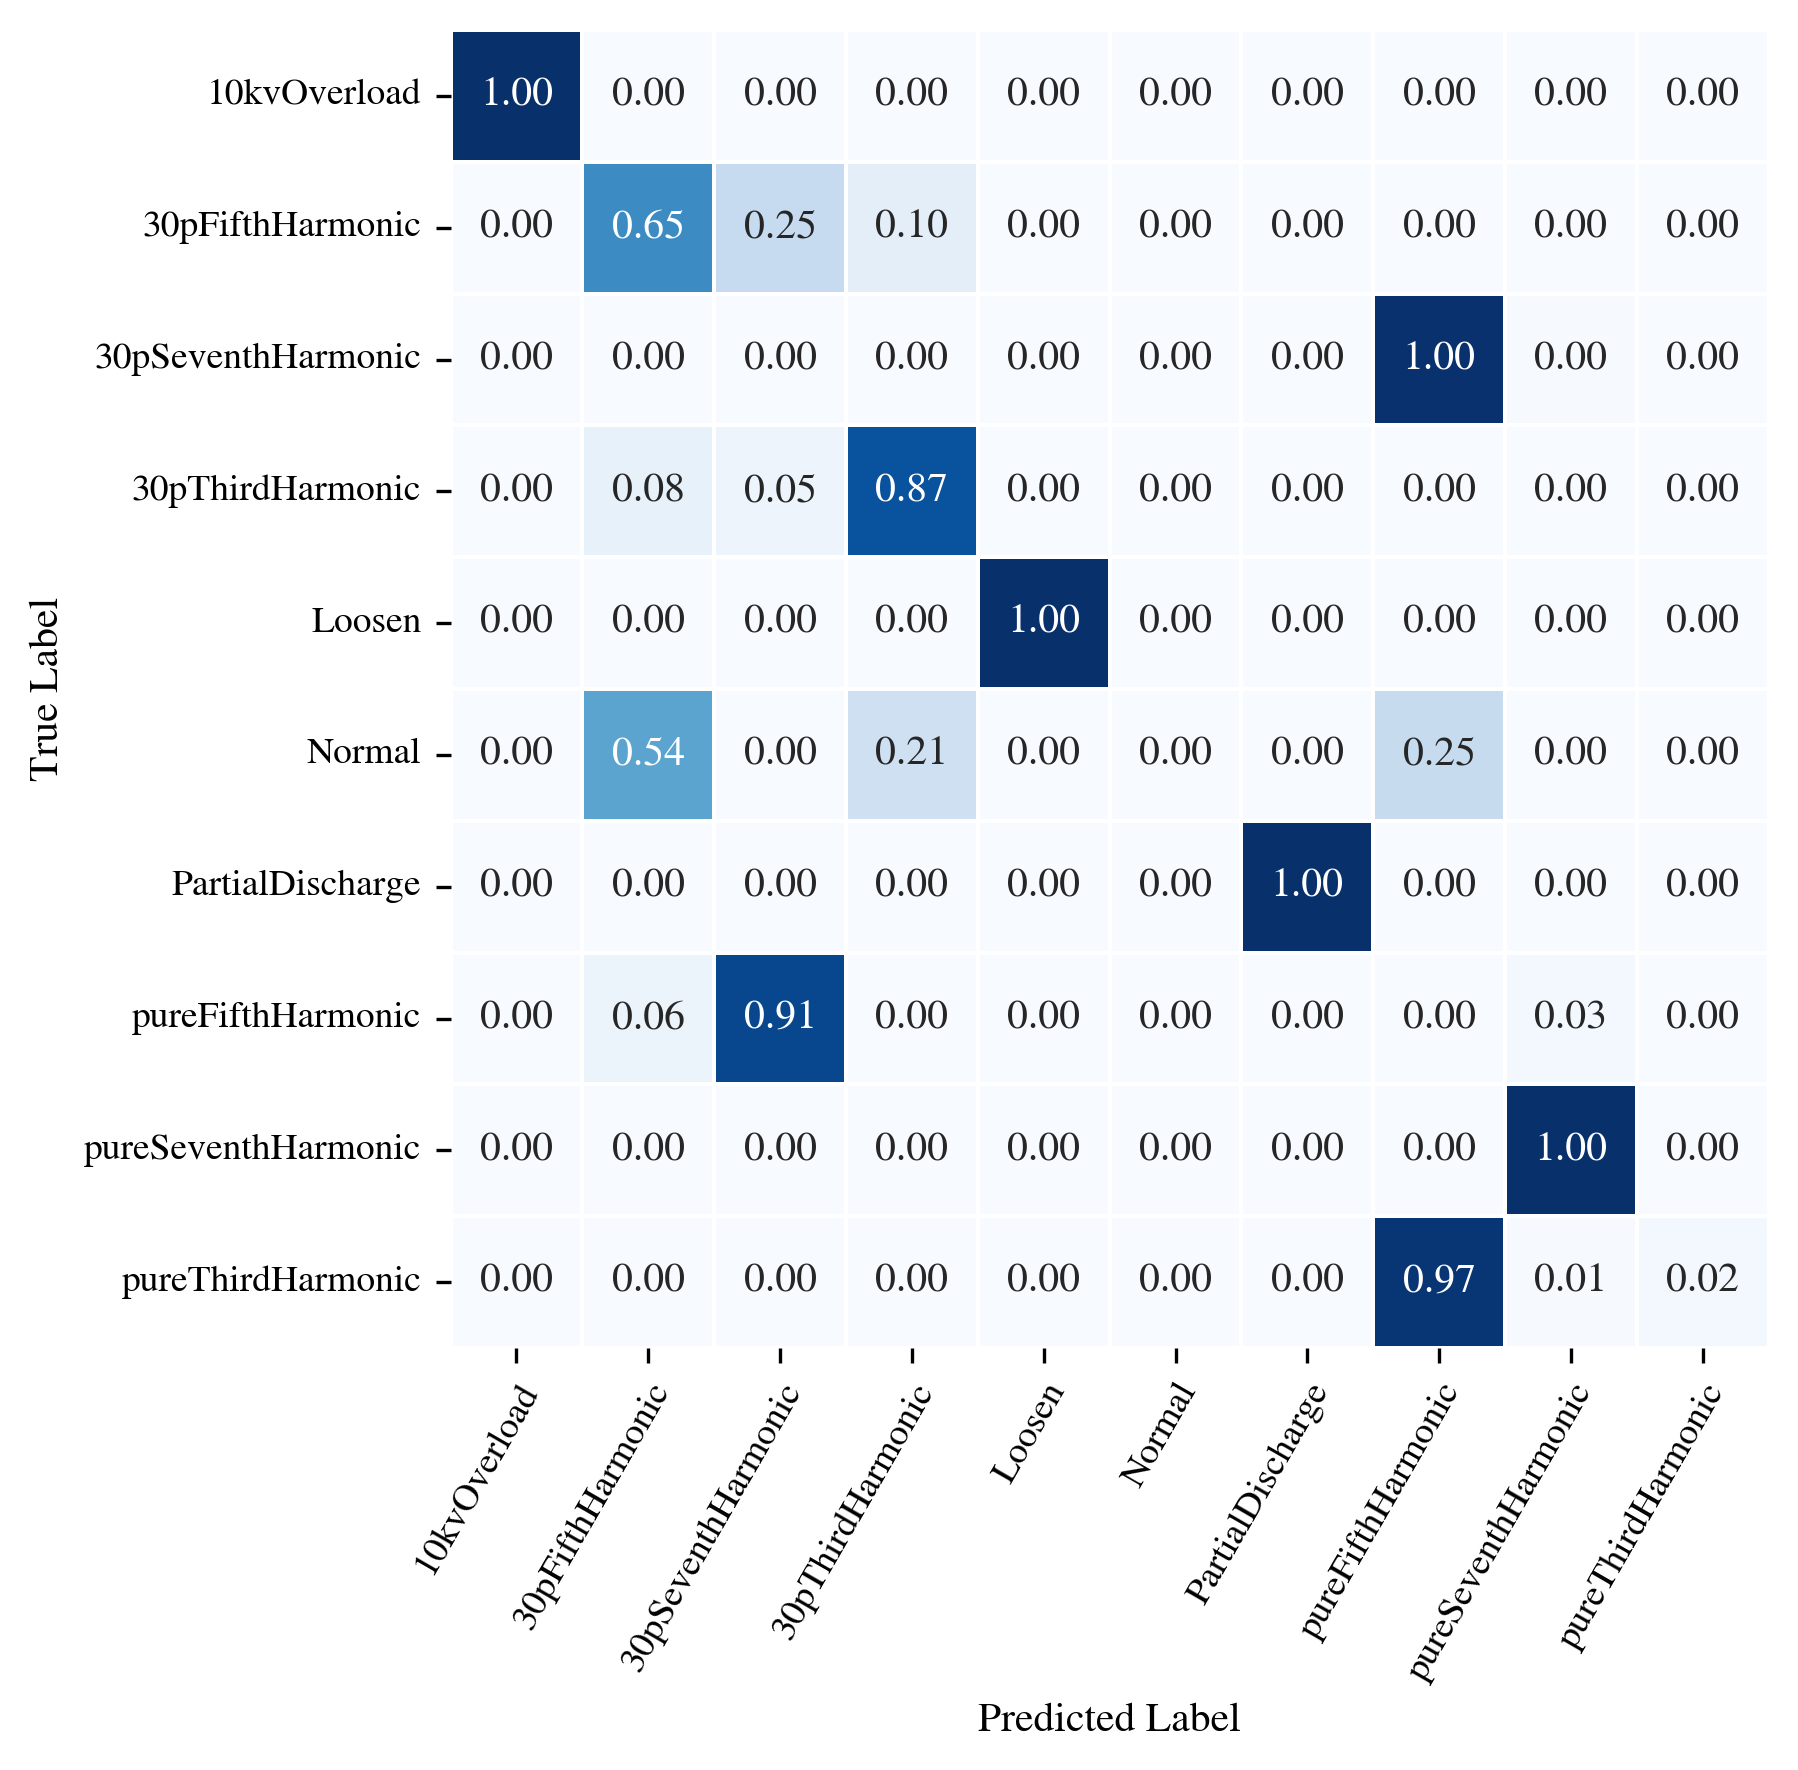
\includegraphics[width=\linewidth]{confusion_matrix/confusion_matrix_vgg16}
% 		\caption{VGG16}
% 	\end{subfigure}
% 	\hfill
% 	\begin{subfigure}{0.32\textwidth}
% 		\centering
% 		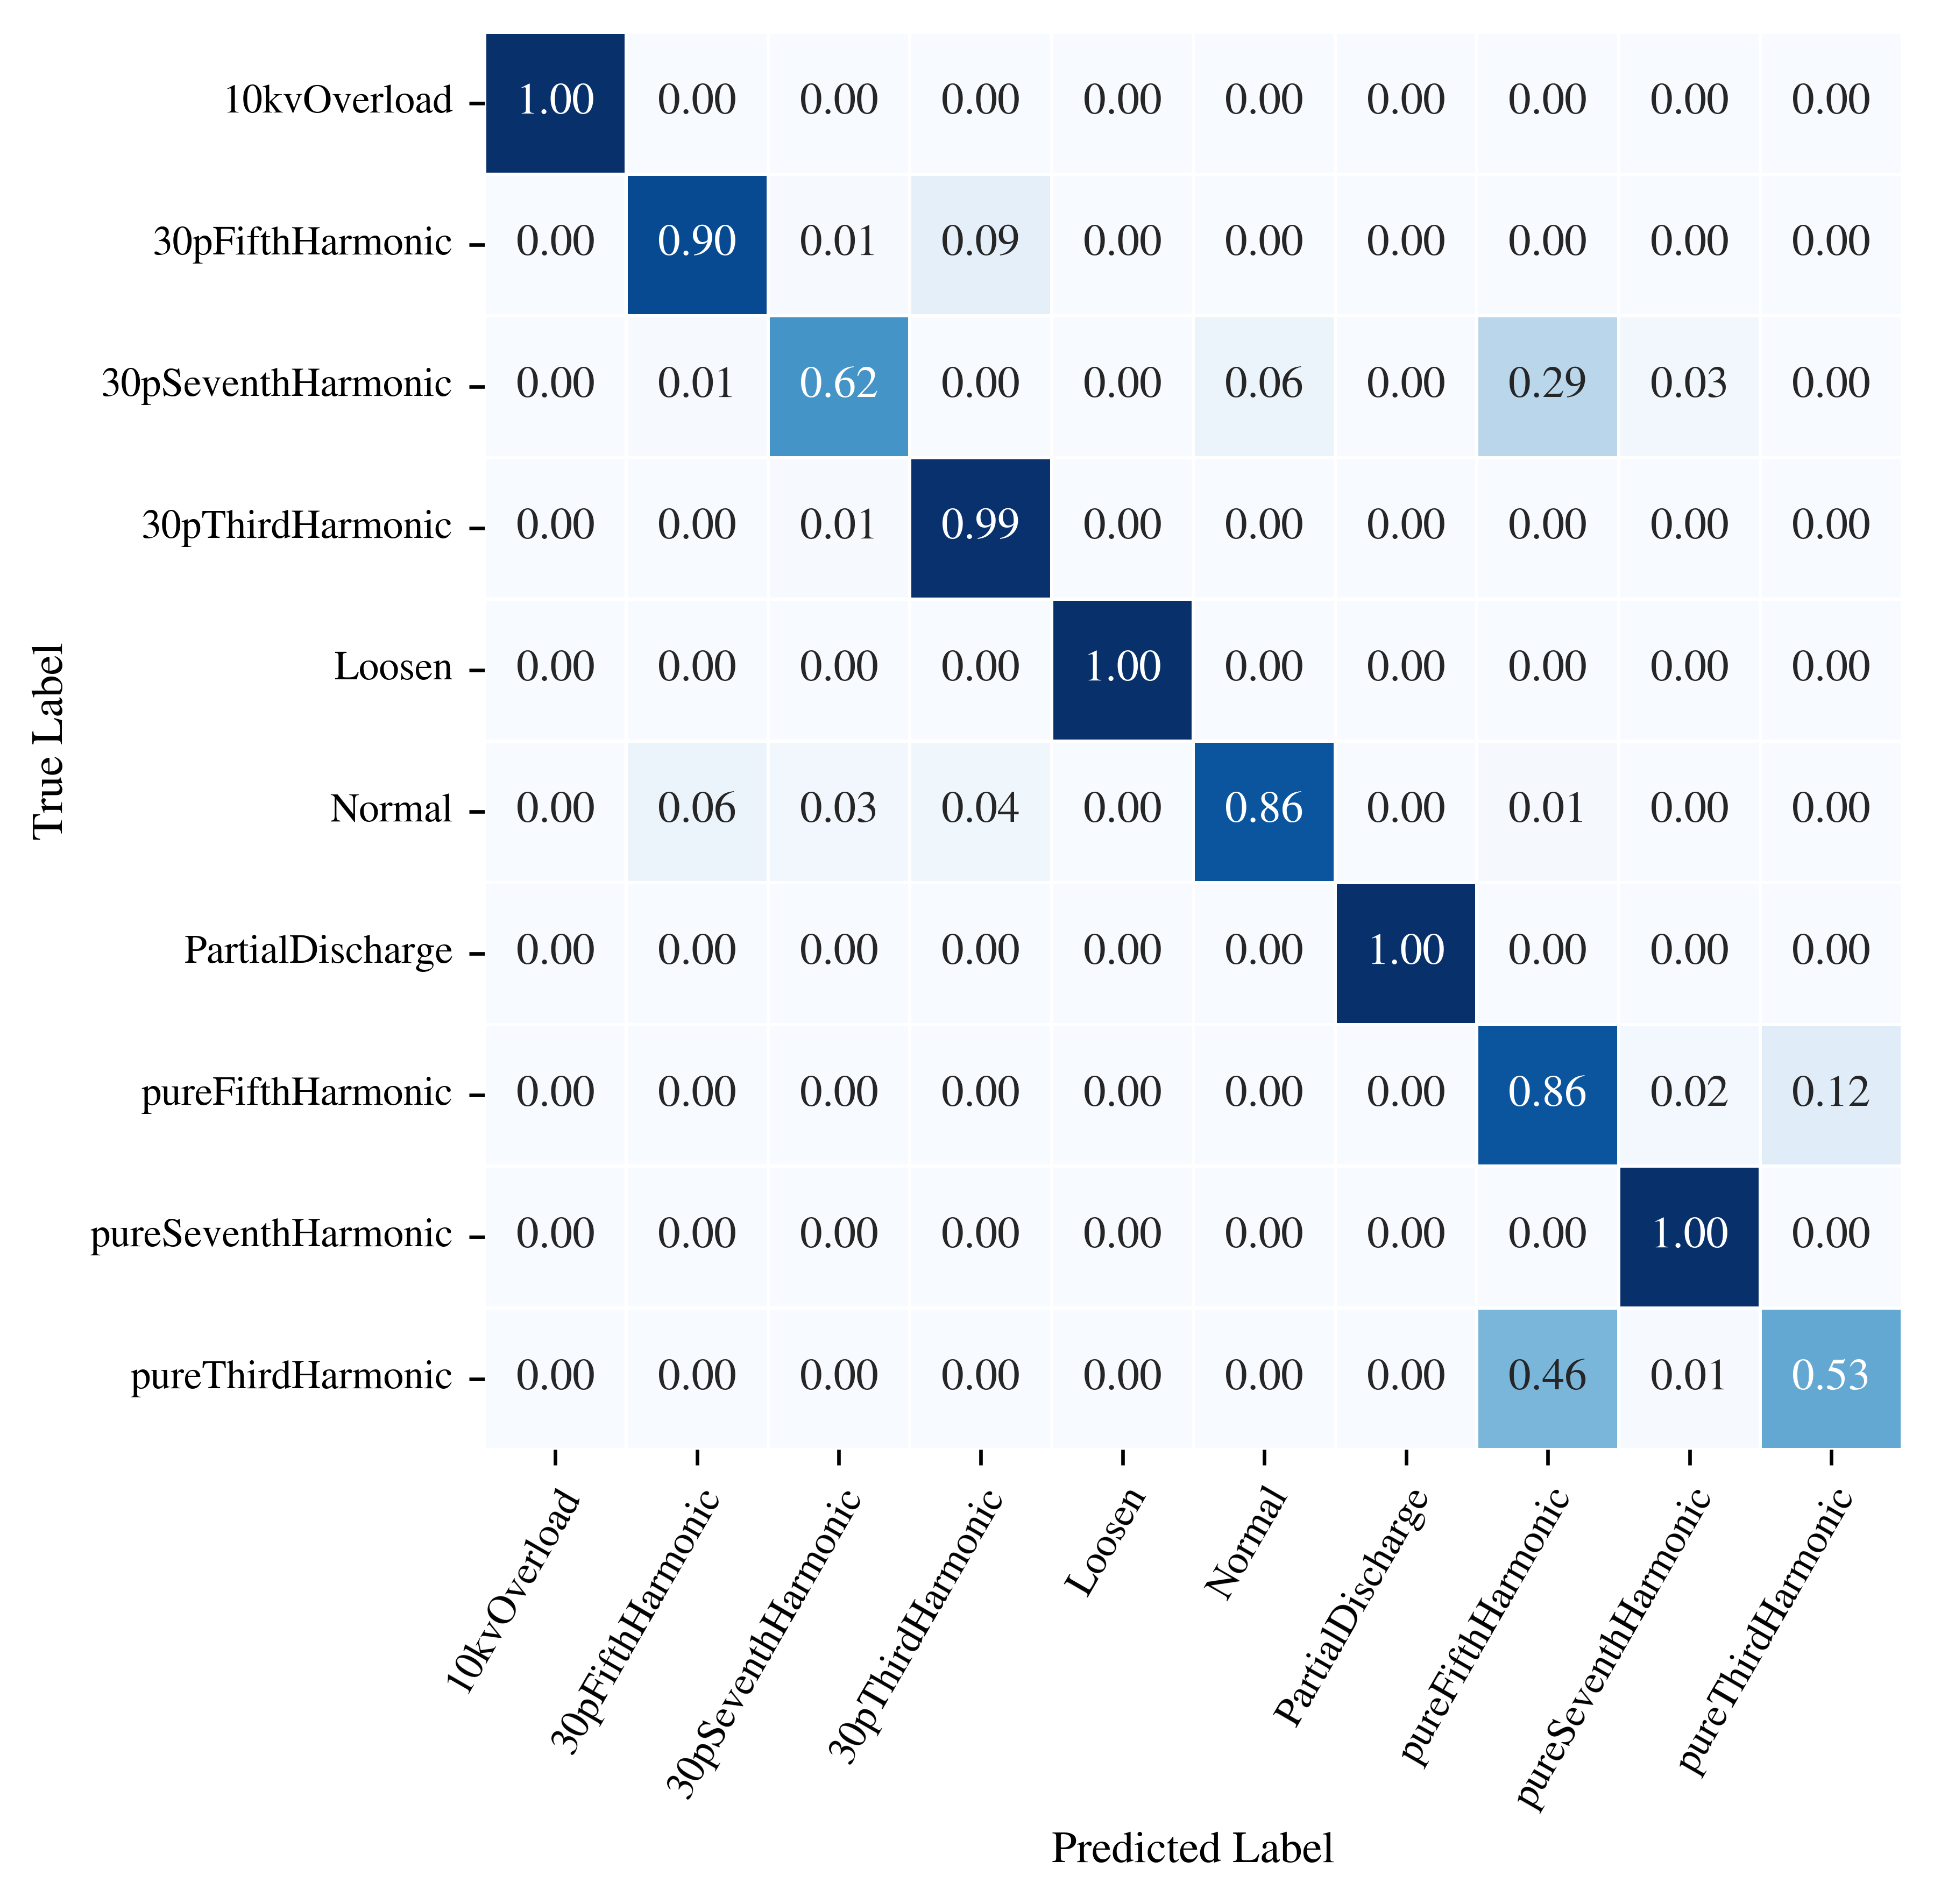
\includegraphics[width=\linewidth]{confusion_matrix/confusion_matrix__MSCA_VGG16}
% 		\caption{MSCA-VGG16 (Ours)}
% 	\end{subfigure}
% 	\caption{Confusion matrices of different network backbones trained using the AW-DPCNN fusion representations. The proposed MSCA-VGG16 achieves the most accurate classification performance with significantly reduced inter-class confusion.}
% 	\label{fig:confusion_matrix}
% \end{figure*}




To evaluate the classification performance of the proposed MSCA-VGG16 model, confusion matrices were employed to visualize the recognition accuracy across ten fault categories, as shown in Fig.~\ref{fig:confusion_matrix}. A hierarchical comparison was conducted among the baseline model, several representative deep learning architectures, and the proposed MSCA-enhanced framework. 

\textbf{1) Performance of the Baseline Model.}
As illustrated in Fig.~\ref{fig:confusion_matrix}(a), the baseline model exhibits limited capability in distinguishing different transformer operating conditions, particularly harmonic-related conditions. Consequently, multiple harmonic-associated states are frequently misclassified. For example, the recognition accuracy of pure third harmonic category is extremely low, with most samples incorrectly classified as pure fifth harmonic category. In addition, the 30\% seventh harmonic category also shows poor performance and is frequently misclassified as pure fifth harmonic category. Similar confusion can be observed between other harmonic conditions, indicating that the baseline network has difficulty capturing subtle spectral differences among harmonic components. These results demonstrate that the baseline architecture lacks sufficient representation capability to effectively discriminate complex acoustic patterns in transformer fault signals.

\textbf{2) Performance of Standard Deep Architectures.}
With the adoption of deeper architectures, including AlexNet, ResNet18, ConvNeXt-Tiny, and VGG16 (Fig.~\ref{fig:confusion_matrix}(b)–(e)), the overall diagnostic performance is noticeably improved compared with the baseline model. The confusion matrices show stronger diagonal dominance, indicating enhanced classification capability across most categories. AlexNet achieves high recognition accuracy for several conditions, such as 30\% fifth harmonic category and pure seventh harmonic category, while misclassification of the normal state remains evident. ResNet18 further improves the recognition of certain harmonic categories, particularly 30\% third harmonic category, although different harmonic components remain difficult to distinguish. ConvNeXt-Tiny and VGG16 exhibit relatively balanced performance across most classes but remain limited in distinguishing acoustically similar harmonic patterns. These observations suggest that although deeper networks strengthen representation capability, accurately discriminating highly similar harmonic signals remains challenging for conventional backbone architectures.

\textbf{3) Superiority of the Proposed MSCA-VGG16 Model.}
As shown in Fig.~\ref{fig:confusion_matrix}(f), the proposed MSCA-VGG16 model achieves the most consistent and accurate classification results among all evaluated architectures. By incorporating the Multi-Scale Convolutional Attention (MSCA) mechanism, the model effectively enhances discriminative representation and suppresses inter-class confusion. Several categories, including 10 kV overload, loosen, partial discharge, and pure seventh harmonic, are recognized with perfect accuracy. Moreover, the recognition performance of previously challenging harmonic-related conditions is significantly improved. For example, the accuracy of the 30\% seventh harmonic category increases to 62\%, while the 30\% third harmonic category reaches 99\% accuracy. Although slight confusion still exists between pure third harmonic and pure fifth harmonic category, the overall confusion pattern is substantially reduced compared with the other backbone networks. These results indicate that the proposed MSCA-VGG16 framework provides more discriminative acoustic representation learning and achieves superior robustness for transformer acoustic fault diagnosis.

\subsection{Ablation Study} 	
To evaluate the effectiveness of the proposed fusion strategy, the AW-DPCNN module is compared with single representation inputs and a naive representation concatenation strategy, as summarized in Table~\ref{tab:fusion_exp_simple}. The experimental observations can be summarized as follows.

\textbf{1) Performance of single-representation inputs.}
When only the Mel spectrogram is used (E1), the model achieves an accuracy of 80.82\% and an F1-score of 77.89\%, indicating limited discriminative capability. When the GADF representation is used alone (E2), the accuracy increases to 85.10\% and the F1-score improves to 86.80\%. This result suggests that the GADF representation captures more discriminative structural patterns for fault identification.

\textbf{2) Impact of naive multi-representation fusion.}
When both Mel and GADF representations are introduced and simply concatenated (E3), the performance does not improve significantly. Although two representations are incorporated, the naive concatenation strategy fails to effectively exploit their complementary characteristics and may introduce redundant or mismatched information.

\textbf{3) Effectiveness of the proposed AW-DPCNN fusion strategy.}
When the proposed AW-DPCNN fusion mechanism is applied (E4), the model achieves the best performance across all evaluation metrics, with an accuracy of 87.45\%, an F1-score of 86.97\%, and a G-mean of 85.69\%. Compared with the naive concatenation strategy (E3), the proposed method improves the accuracy by 5.25 percentage points.

\textbf{4) Overall performance analysis.}
The results indicate that adaptive multi-representation fusion is more effective than simple feature aggregation. By dynamically adjusting the contribution of heterogeneous acoustic representations, the AW-DPCNN module can better exploit complementary information and enhance discriminative representation learning for transformer fault diagnosis.

\begin{figure}[!htbp]
	\centering
	\begin{subfigure}{0.48\textwidth}
		\centering
		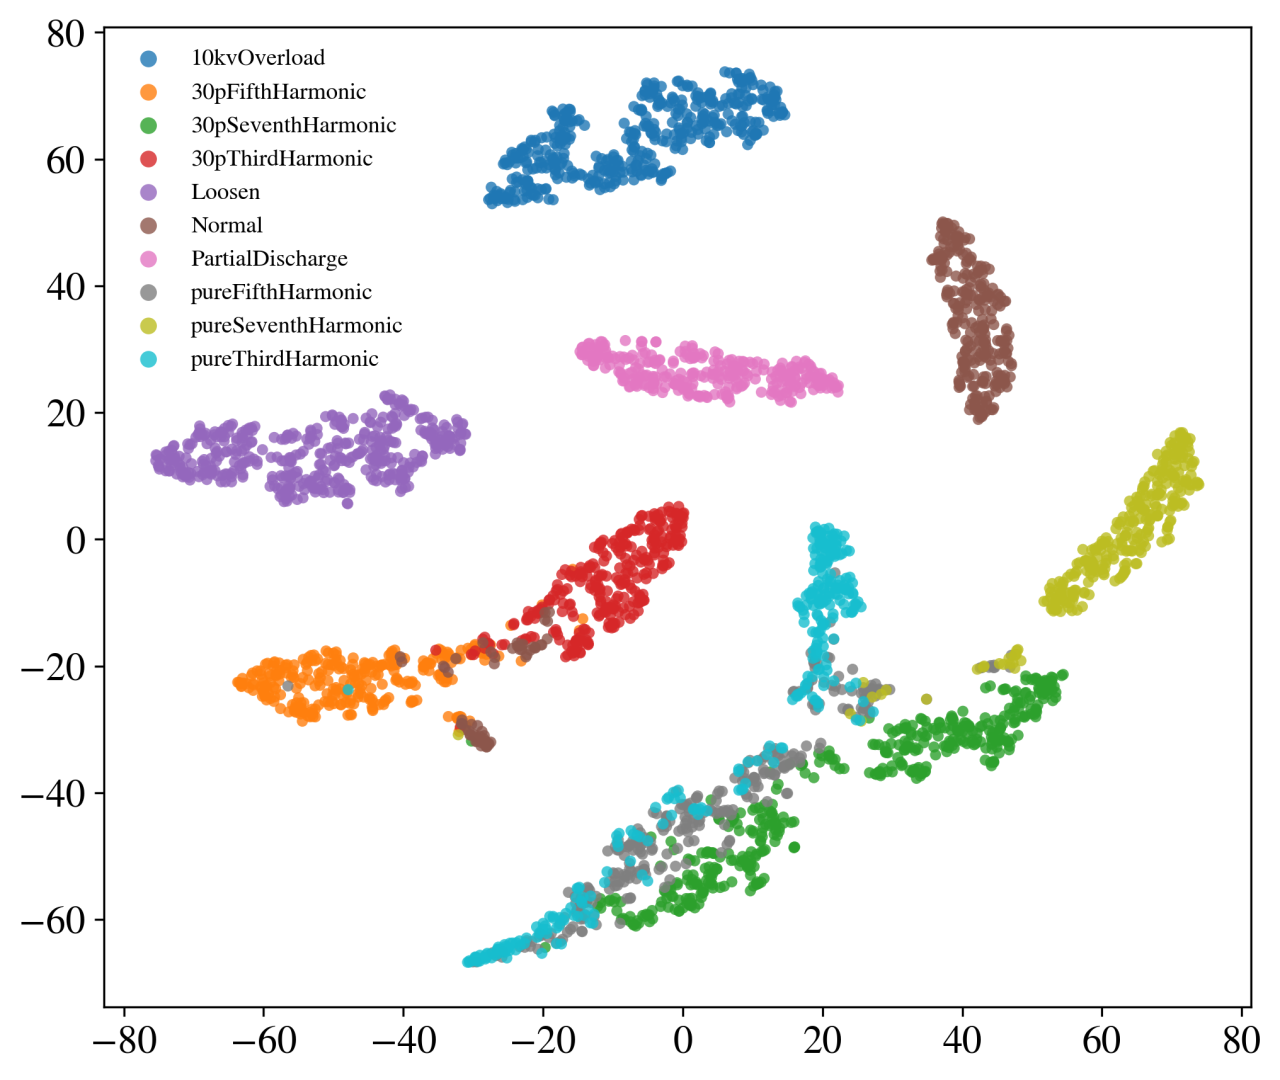
\includegraphics[width=\linewidth]{tsne/tsne__MSCA_VGG16_mel}
		\caption{Mel}
		\label{subfig:tsne_msca_vgg16_mel}
	\end{subfigure}
	\hfill
	\begin{subfigure}{0.48\textwidth}
		\centering
		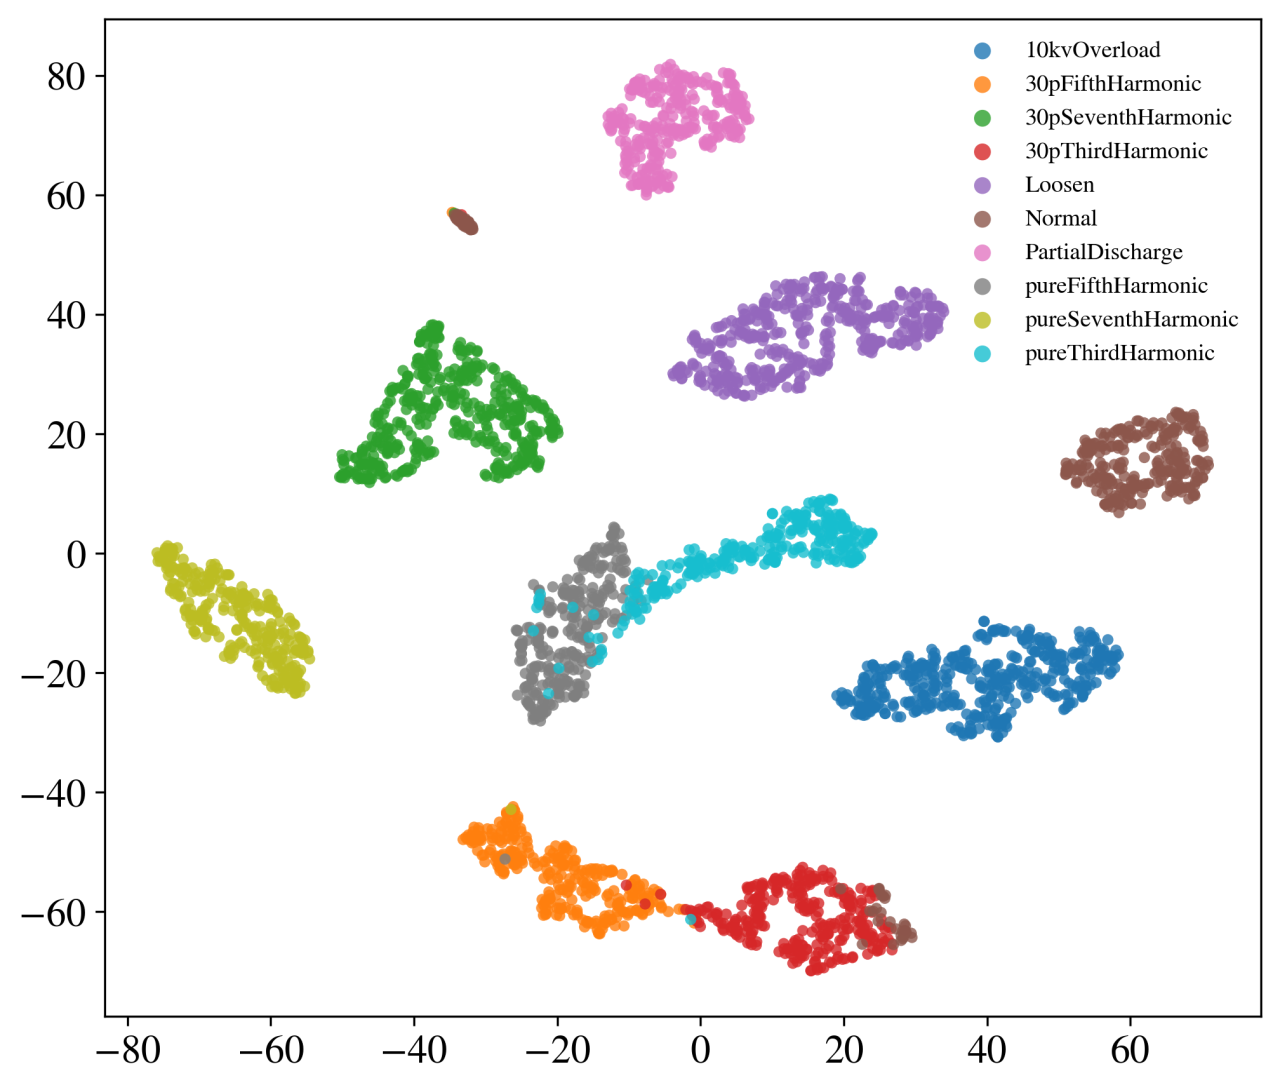
\includegraphics[width=\linewidth]{tsne/tsne__MSCA_VGG16_gadf}
		\caption{GADF}
		\label{subfig:tsne_msca_vgg16_gadf}
	\end{subfigure}\\[3mm]

	\begin{subfigure}{0.48\textwidth}
		\centering
		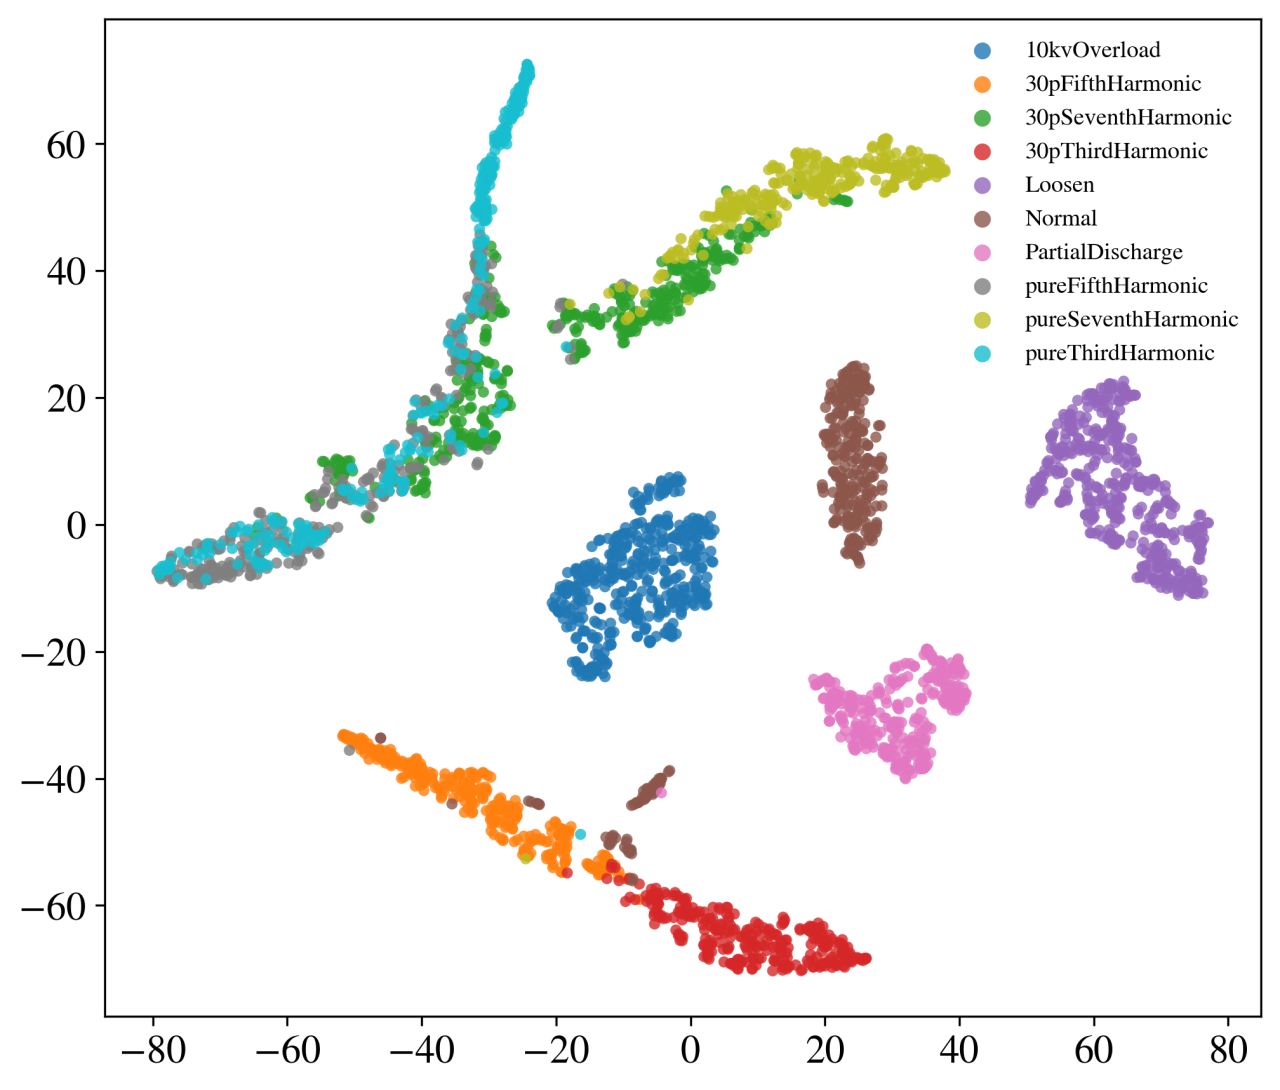
\includegraphics[width=\linewidth]{tsne/tsne__MSCA_VGG16_concat}
		\caption{Concat}
		\label{subfig:tsne_msca_vgg16_concat}
	\end{subfigure}
	\hfill
	\begin{subfigure}{0.48\textwidth}
		\centering
		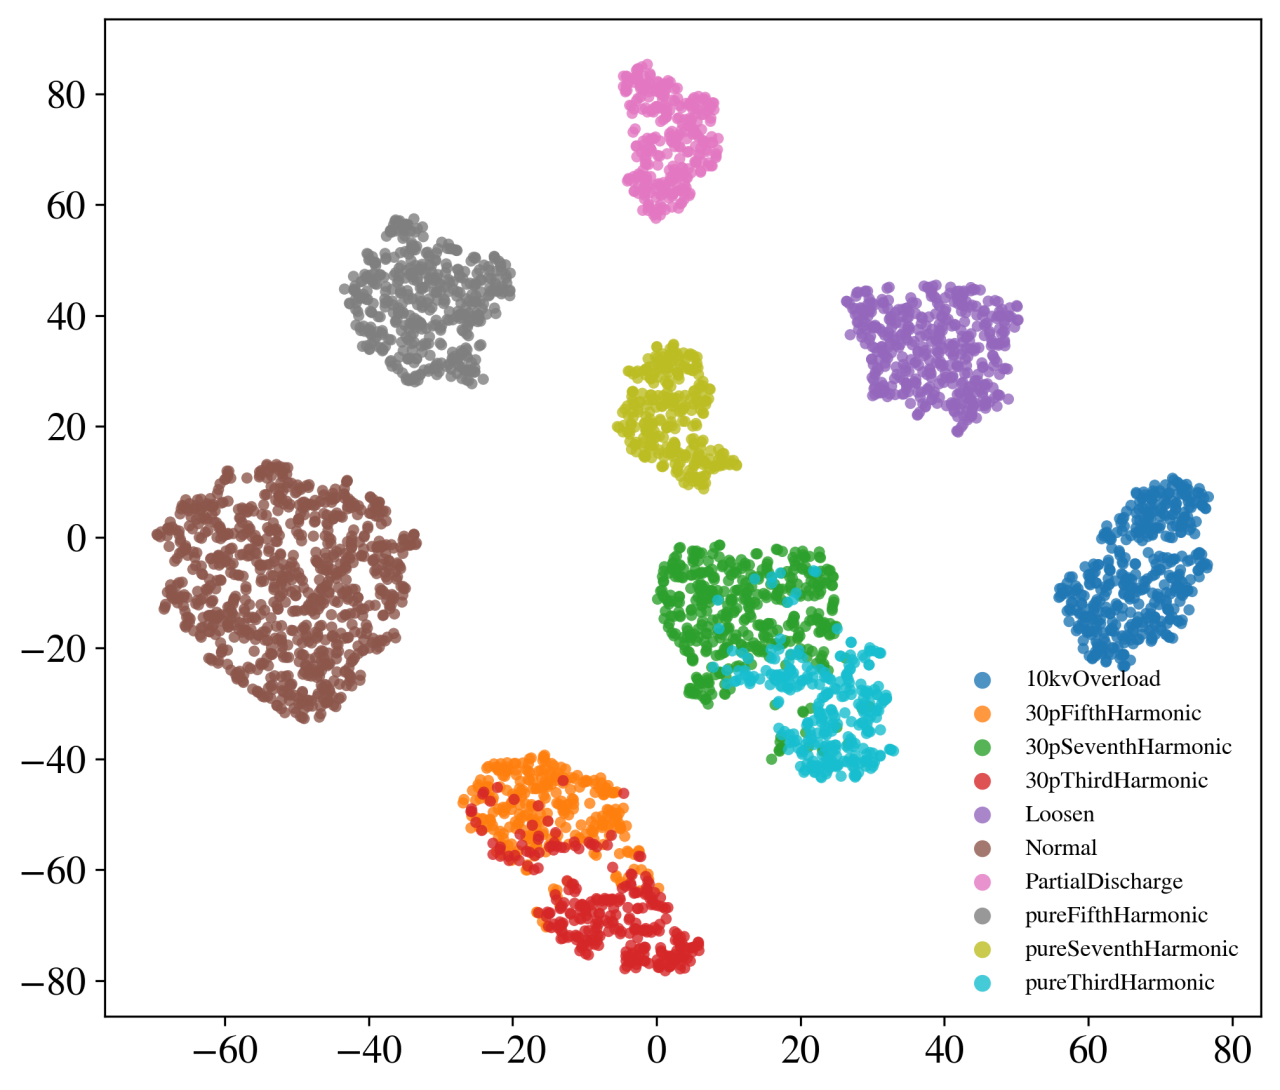
\includegraphics[width=\linewidth]{tsne/tsne__MSCA_VGG16_awdpcnn}
		\caption{AW-DPCNN (Ours)}
		\label{subfig:tsne_msca_vgg16_awdpcnn}
	\end{subfigure}
	\caption{t-SNE visualization of feature distributions under different fusion mechanisms. (a) E1: Mel features. (b) E2: GADF features. (c) E3: Mel+GADF with concatenation fusion. (d) E4: Mel+GADF with the proposed AW-DPCNN fusion.}
	\label{Fig:tsne}
	\vspace{-5pt}
\end{figure}





\begin{table}
	\centering
	\caption{Comparison of Fusion Strategies}
	\begin{tabular}{lccccccc}
		\toprule
		\textbf{Exp.} & \textbf{Representation} & \textbf{Mel} & \textbf{GADF} & \textbf{Fusion Strategy} 
		& \textbf{Acc (\%)} & \textbf{F1 (\%)} & \textbf{G-mean (\%)} \\
		\midrule
		E1 & Mel      & $\checkmark$ & $\times$ & None  
		& 80.82 & 77.89 & 49.68 \\
		E2 & GADF     & $\times$ & $\checkmark$ & None 
		& 85.10 & 86.80 & 81.08 \\
		E3 & Mel+GADF & $\checkmark$ & $\checkmark$ & Concat 
		& 82.20 & 83.50 & 81.08 \\
		E4 & Mel+GADF & $\checkmark$ & $\checkmark$ & \textbf{AW-DPCNN (Ours)} 
		& \textbf{87.45} & \textbf{86.97} & \textbf{85.69} \\
		\bottomrule
	\end{tabular}
	\label{tab:fusion_exp_simple}
\end{table}



In addition to the quantitative metrics derived from the confusion matrix, t-SNE visualization is applied to the feature embeddings extracted before the final classification layer, as illustrated in Fig. \ref{Fig:tsne}. The visualization results for Exp. 1–Exp. 4 defined in Table \ref{tab:fusion_exp_simple} show that the proposed AW-DPCNN fusion yields the most compact intra class clusters and the clearest inter class separation.

\begin{figure}
	\centering

	\begin{subfigure}{0.48\textwidth}
		\centering
		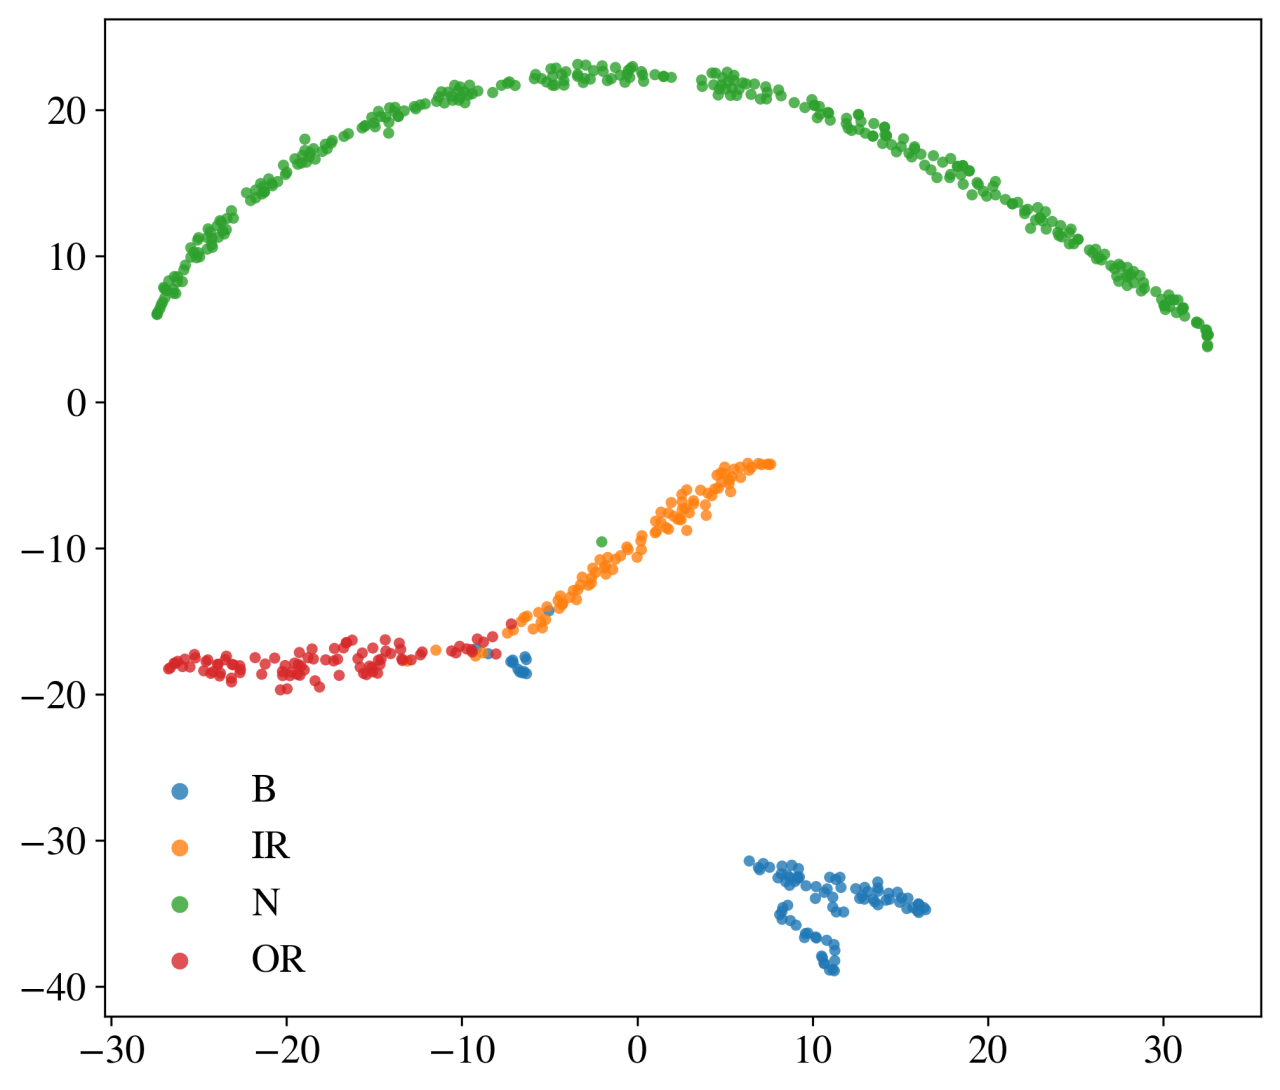
\includegraphics[width=\linewidth]{tsne_cwru/tsne_cwru_mel}
		\caption{Mel}
		\label{subfig:tsne_cwru_mel}
	\end{subfigure}
	\hfill
	\begin{subfigure}{0.48\textwidth}
		\centering
		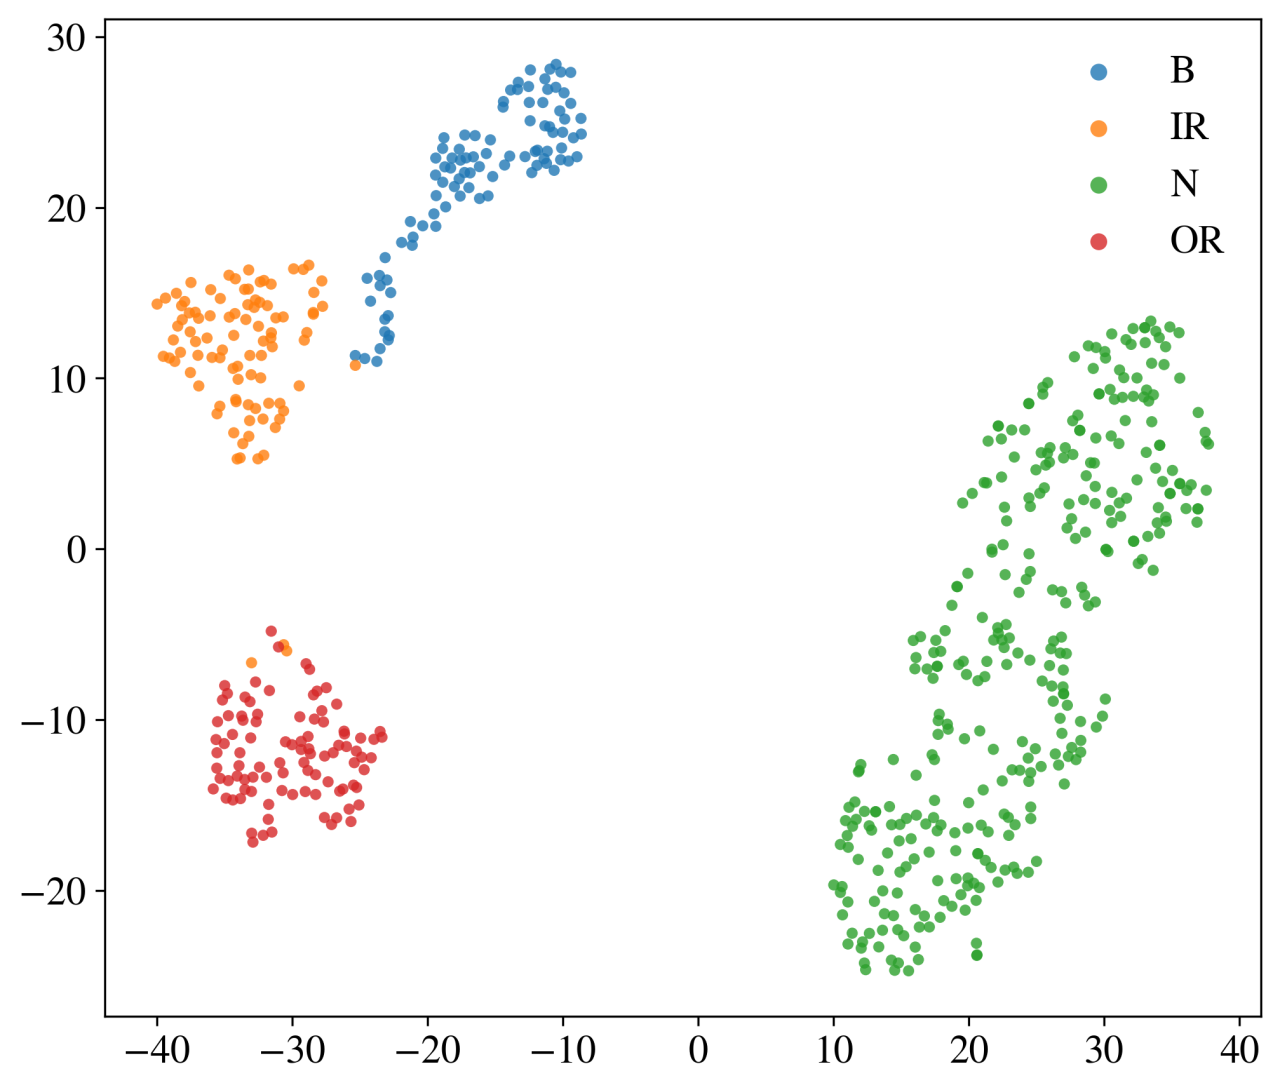
\includegraphics[width=\linewidth]{tsne_cwru/tsne_cwru_gadf}
		\caption{GADF}
		\label{subfig:tsne_cwru_gadf}
	\end{subfigure}\\[3mm]

	\begin{subfigure}{0.48\textwidth}
		\centering
		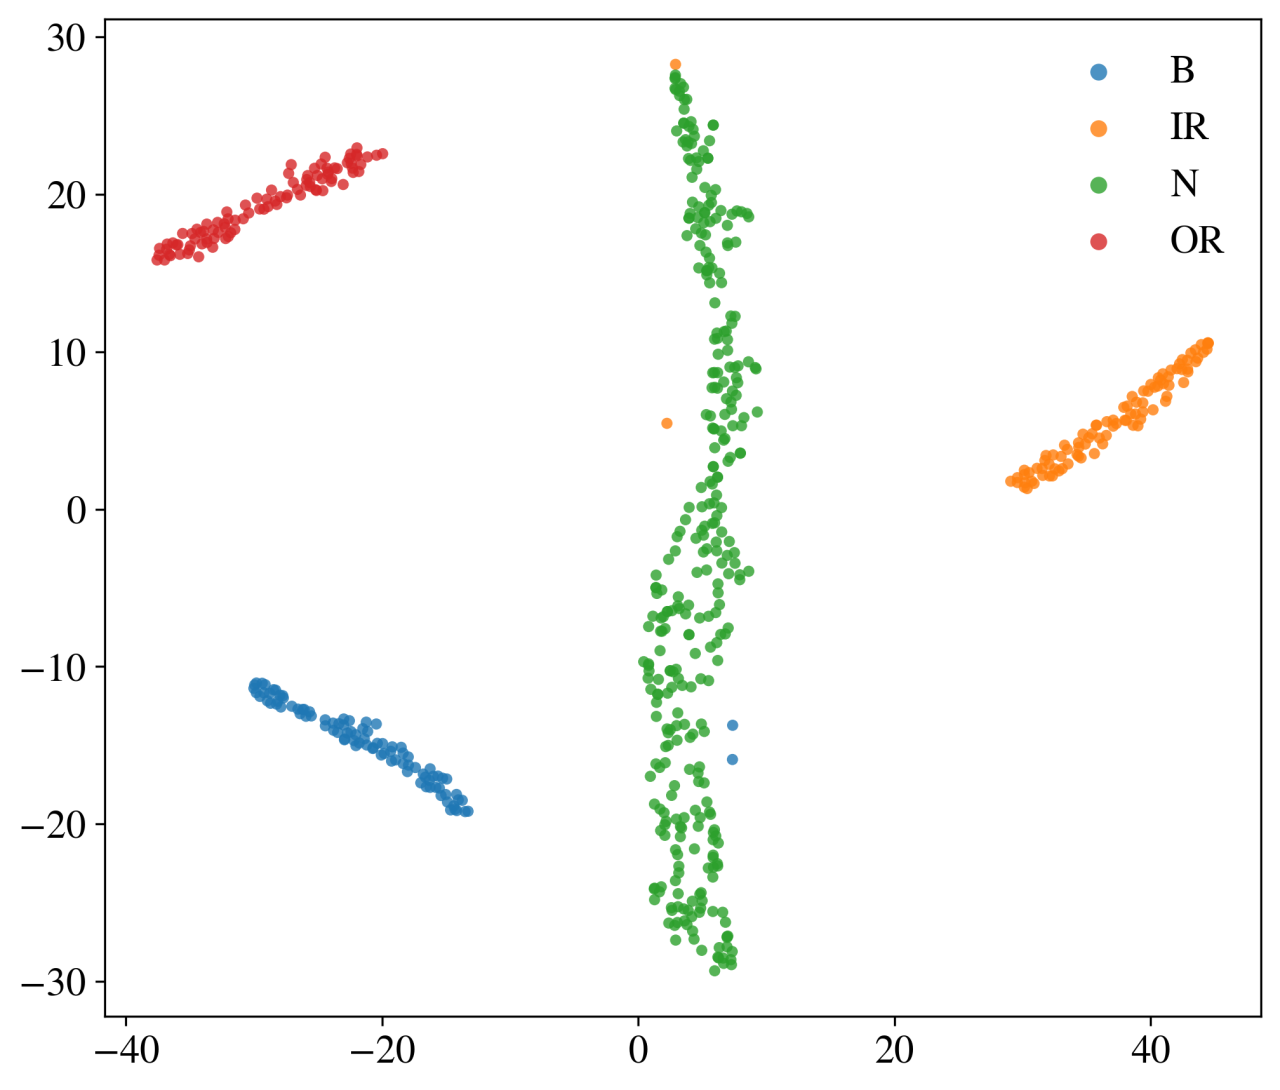
\includegraphics[width=\linewidth]{tsne_cwru/tsne_cwru_concat}
		\caption{Concat}
		\label{subfig:tsne_cwru_concat}
	\end{subfigure}
	\hfill
	\begin{subfigure}{0.48\textwidth}
		\centering
		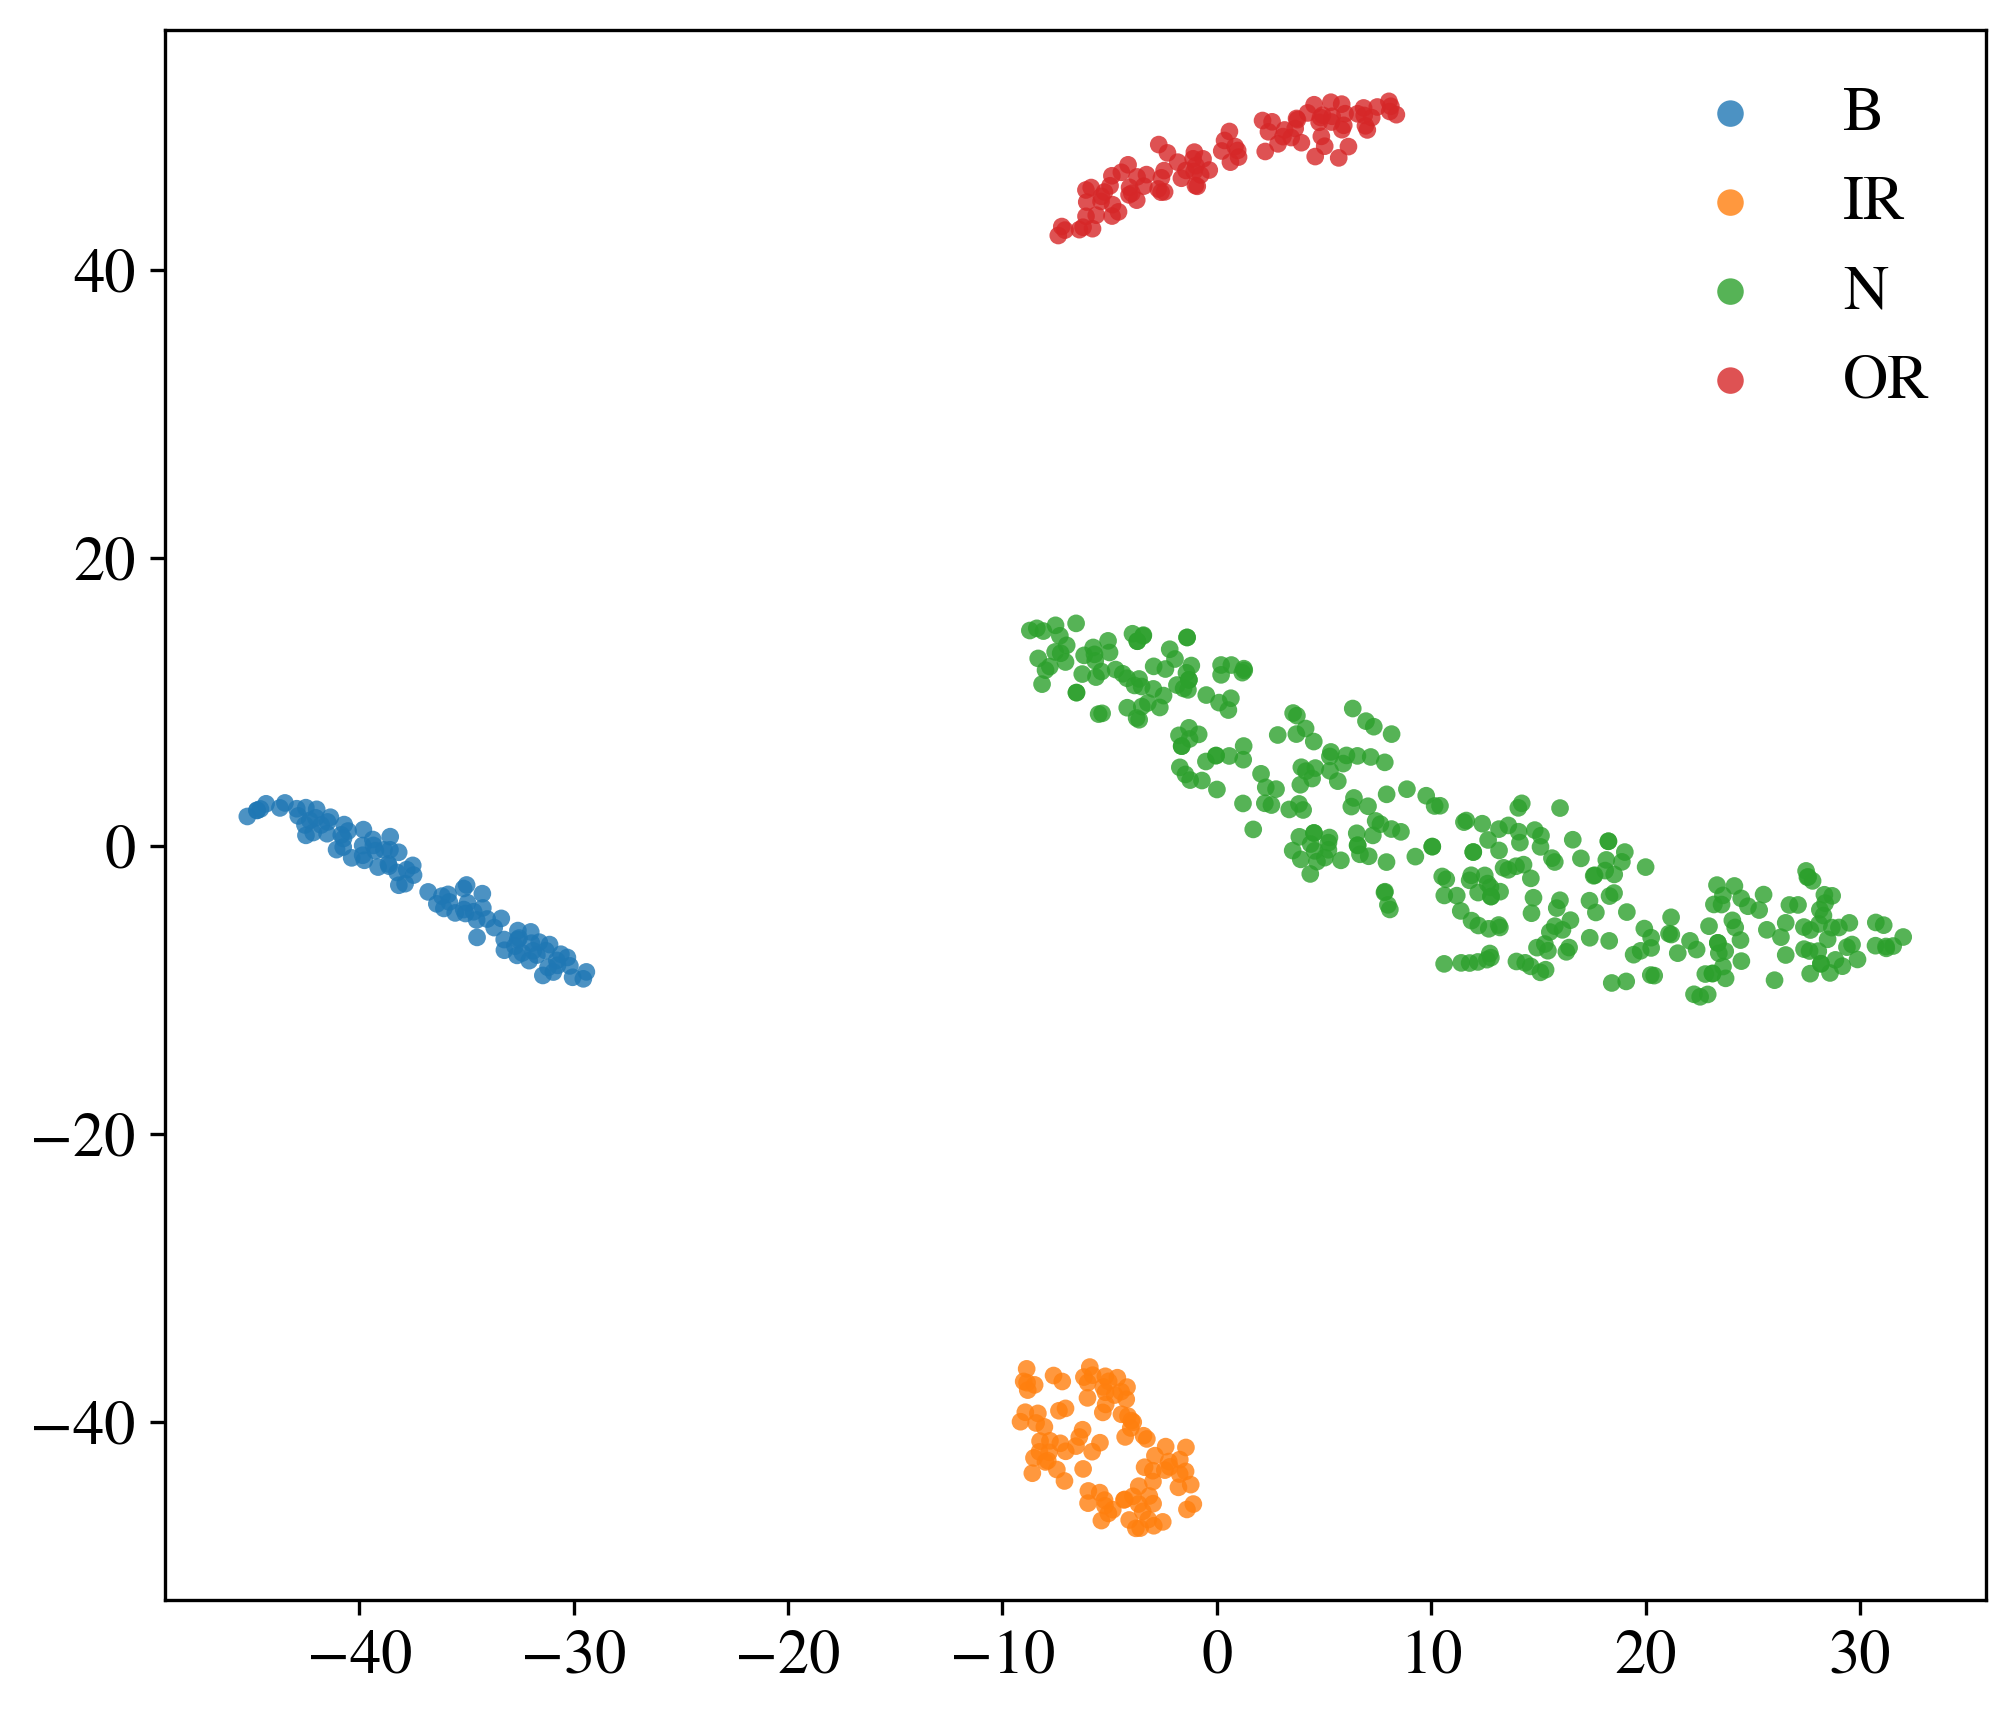
\includegraphics[width=\linewidth]{tsne_cwru/tsne_cwru_awdpcnn}
		\caption{AW-DPCNN(Ours)}
		\label{subfig:tsne_cwru_awdpcnn}
	\end{subfigure}

	\caption{
		t-SNE visualization of feature distributions under different strategies. (a) A1: Mel representation. (b) A2: GADF representation. (c) A3: Mel+GADF with concatenation fusion. (d) A4: Mel+GADF with the proposed AW-DPCNN fusion, which produces more compact intra-class clusters and clearer inter-class boundaries.
	}

	\label{Fig:tsne_CWRU}

	\vspace{-3mm}

\end{figure}

To analyze the contribution of each architectural component, an ablation study was conducted on VGG16-based models, as summarized in Table~\ref{tab:ablation_vgg16}. The baseline VGG16 (M1) achieves an accuracy of 78.15\% and an F1-score of 75.82\%, indicating limited discriminative capability for acoustic fault diagnosis. Introducing individual components, including channel attention (M2), multi-scale convolution (M3), and the compact embedding head (M4), all leads to performance improvements compared with the baseline, demonstrating the effectiveness of each module in enhancing representation. When all proposed components are integrated, the full MSCA-VGG16 model (M5) achieves the best performance with an accuracy of 87.45\% and an F1-score of 86.97\%. Meanwhile, the Kappa coefficient increases from 75.76\% in the baseline model to 86.03\%, indicating a higher level of agreement between the predicted labels and ground truth. The consistent improvement across all evaluation metrics indicates that the multi-scale feature enhancement, channel attention mechanism, and compact embedding head work cooperatively to strengthen discriminative representation learning and improve diagnostic performance.

\begin{table}
	\centering
	\caption{Ablation Study on VGG16-Based Models. MS: Multi-Scale; CA: Channel Attention; EH: Embedding Head.}
	\label{tab:ablation_vgg16}
	\renewcommand{\arraystretch}{1.2}
	\small
		\begin{tabular}{lccccccc}
			\hline
			\textbf{Exp.} & \textbf{MS} & \textbf{CA} & \textbf{EH} & \textbf{Acc} & \textbf{F1} & \textbf{Kappa} & \textbf{G-mean} \\
			\hline
			M1 & $\times$ & $\times$ & $\times$ & 78.15 & 75.82 & 75.76 & 57.37 \\
			M2 & $\times$ & $\checkmark$ & $\times$ & 82.87 & 81.59 & 80.99 & 77.74 \\
			M3 & $\checkmark$ &$\times$ & $\times$ & 80.00 & 79.10 & 77.81 & 65.51 \\
			M4 & $\times$ & $\times$ & $\checkmark$ & 81.32 & 80.10 & 79.27 & 71.81 \\
			\textbf{M5} & $\checkmark$ & $\checkmark$ & $\checkmark$ & \textbf{87.45} & \textbf{86.97} & \textbf{86.03} & \textbf{85.69} \\
			\hline
		\end{tabular}
\end{table}



\subsection{Generalization Validation on the CWRU Dataset}
To further evaluate the generalization capability of the proposed method, experiments were conducted on the publicly available Case Western Reserve University (CWRU) bearing dataset. The 12 kHz drive-end vibration signals were selected, including four conditions: Normal (N), Inner race fault (IR), Outer race fault (OR, located at the load zone at 6 o’clock), and Ball fault (B), all with a fault diameter of 0.007 inches. The vibration signals were converted into Mel spectrograms and GADF images using the same preprocessing pipeline as that applied to the transformer acoustic signals. To provide a fair evaluation of cross-domain generalization, no dataset-specific parameter tuning was performed. A cross-speed evaluation strategy was adopted, where samples with a fault diameter of 0.007 inches were used for training and those with 0.014 inches were used for testing, while ensuring that segments from the same raw signal were assigned exclusively to one subset to prevent data leakage. Although the CWRU dataset is based on vibration signals rather than acoustic signals, it provides a widely used benchmark for evaluating the generalization capability of fault diagnosis models.

As summarized in Table~\ref{tab:cwru_ablation}, the single-representation (A1 and A2) achieves relatively limited performance, with accuracies of 89.72\% and 91.34\%, respectively, indicating that Mel or GADF representations alone cannot fully characterize the fault information. When the two representations are directly fused through feature concatenation (A3), the accuracy increases to 96.41\%, demonstrating that the Mel spectrogram and GADF representations provide complementary information. By introducing the proposed AW-DPCNN fusion strategy (A4), the accuracy further improves to 97.86\%, showing that adaptive weighted fusion can better exploit cross-modal representation correlations than simple concatenation. Finally, combining AW-DPCNN with the MSCA-VGG16 classifier (A5) achieves the best performance with an accuracy of 99.67\%.

\begin{table}
\caption{
	Validation on the Public CWRU Dataset.
	Rep.: Representation;
	Prec.: Precision;
	Rec.: Recall;
	Gm.: G-mean.
}
	\label{tab:cwru_ablation}
	\centering
	\renewcommand{\arraystretch}{1.2}
	
	\resizebox{\linewidth}{!}{
		\begin{tabular}{lcccccccc}
			\toprule
			\textbf{Exp.} &
			\textbf{Rep.} &
			\textbf{Fusion} &
			\textbf{Network} &
			\textbf{Acc} &
			\textbf{Prec.} &
			\textbf{Rec.} &
			\textbf{F1} &
			\textbf{Gm.} \\
			\midrule
			
			A1 & Mel & None & Backbone & 89.72 & 88.94 & 83.76 & 85.42 & 80.31 \\
			
			A2 & GADF & None & Backbone & 91.34 & 90.38 & 85.90 & 84.95 & 82.05 \\
			
			A3 & Mel+GADF & Concat & Backbone & 96.41 & 94.60 & 94.53 & 94.42 & 94.53 \\
			
			A4 & Mel+GADF & \textbf{AW-DPCNN} & Backbone & 97.86 & 96.42 & 96.85 & 96.88 & 96.91 \\
			
			A5 & Mel+GADF & AW-DPCNN & \textbf{MSCA-VGG16} & \textbf{99.67} & \textbf{99.48} & \textbf{99.47} & \textbf{99.47} & \textbf{99.46} \\
			
			\bottomrule
		\end{tabular}
	}
\end{table}




The t-SNE visualization results in Fig.~\ref{Fig:tsne_CWRU} further support these findings. Compared with the scattered distributions of the single representation and the partially overlapping clusters under concatenation fusion, the features produced by AW-DPCNN exhibit more compact intra-class distributions and clearer inter-class boundaries. This demonstrates that the proposed AW-DPCNN effectively enhances the discriminative capability of fused acoustic representations.

\section{Conclusion}
\label{section6}
To overcome the limitations of single-representation and low accuracy in transformer fault diagnosis, this study integrates Mel spectrograms with GADF images. This combination captures complementary time–frequency and angular-domain representations from acoustic signals, forming a more comprehensive basis for fault identification. An AW-DPCNN is introduced to effectively fuse the heterogeneous representations by modeling cross-domain correlations while suppressing redundant and noise-sensitive components. On this basis, an MSCA-VGG16 network is designed as the classification backbone to further strengthen discriminative representation learning across multiple receptive fields and frequency scales. By jointly leveraging multi-representation fusion and attention-guided deep feature extraction, the proposed framework improves diagnostic robustness under complex operating conditions and acoustic disturbances. To further validate the effectiveness and generalization capability of the proposed method, experiments are also conducted on the CWRU bearing dataset. The results demonstrate consistent improvements in classification performance across different backbones, highlighting the compatibility and robustness of the proposed approach and confirming its effectiveness in addressing the low diagnostic accuracy commonly observed in existing fault diagnosis models.

In future work, we aim to further optimize the proposed framework to improve recognition accuracy under more diverse and complex operating conditions, with the ultimate goal of enhancing the reliability and applicability of intelligent transformer faults diagnosis systems.

\bibliography{references}

\bibliographystyle{iopart-num}


\end{document}


